\documentclass[]{article}
\usepackage{hyperref}
\usepackage{multirow}
\usepackage{float}
\usepackage{textcomp}
\usepackage{graphicx}
\usepackage{float}
% Title Page
\title{Low-Comotovation: System Design Document}
\author{}
\date{}

\begin{document}

\maketitle
\tableofcontents
\titlepage

\subsection{Versioning \& Authorship}
Version 0.1
\newline
Low-Comotovation \textcopyright

\raggedright
Software Design Specification: Low-Comotovation \\
Status: Preliminary Release: Software Design Review

\subsection{References}
During the development of this document, IEEE 1016 was utilized.

\subsection{Purpose}
This document will specify the architecture and design of the Low-Comotovation train system. It shall discuss the structural and design and considerations of the train system and the accompanying subsystems of the train system. It shall also detail design considerations in vital subsystems.

\subsection{Stakeholders \& Concerns}
The stakeholders of this document are anticipated to be the following:
\begin{itemize}
	\item Future Design Teams: Future design teams are anticipated to utilize this document to guide their usage of the track controller system
	\item Pittsburgh Rail Company: The rail company utilizing the Software Design Specification (SDS) to guide the development of physical systems associated with the software
\end{itemize}

Future design teams associated with the continued development benefit from increased documentation of the original system by allowing for more efficient software design procedures in future revision by potentially unrelated developers.

The benefits to the Pittsburgh Rail Company from  a detailed software design specification are twofold. First, a detailed SDD provides developers of railway hardware the information required to produced a paired system. Second, a documented SDD allows the Pittsburgh Rail Company to evaluate the designs ability to meet specifications for vitality.

\section{Introduction}
To ensure safe, predictable, and reliable operation of the system, there are three primary considerations:
\begin{enumerate}
	\item \emph{Vitality:} Vitality of a system within this document refers to a safety-critical system.
	\item \emph{Testability:} Any system implemented must be easily tested to ensure reliability
	\item \emph{Modularity:} Any system designed must reuse code wherever possible
\end{enumerate}

\section{System Design Use Cases}
The overall system diagram is as follows:
\begin{figure}[H]
	\centering
	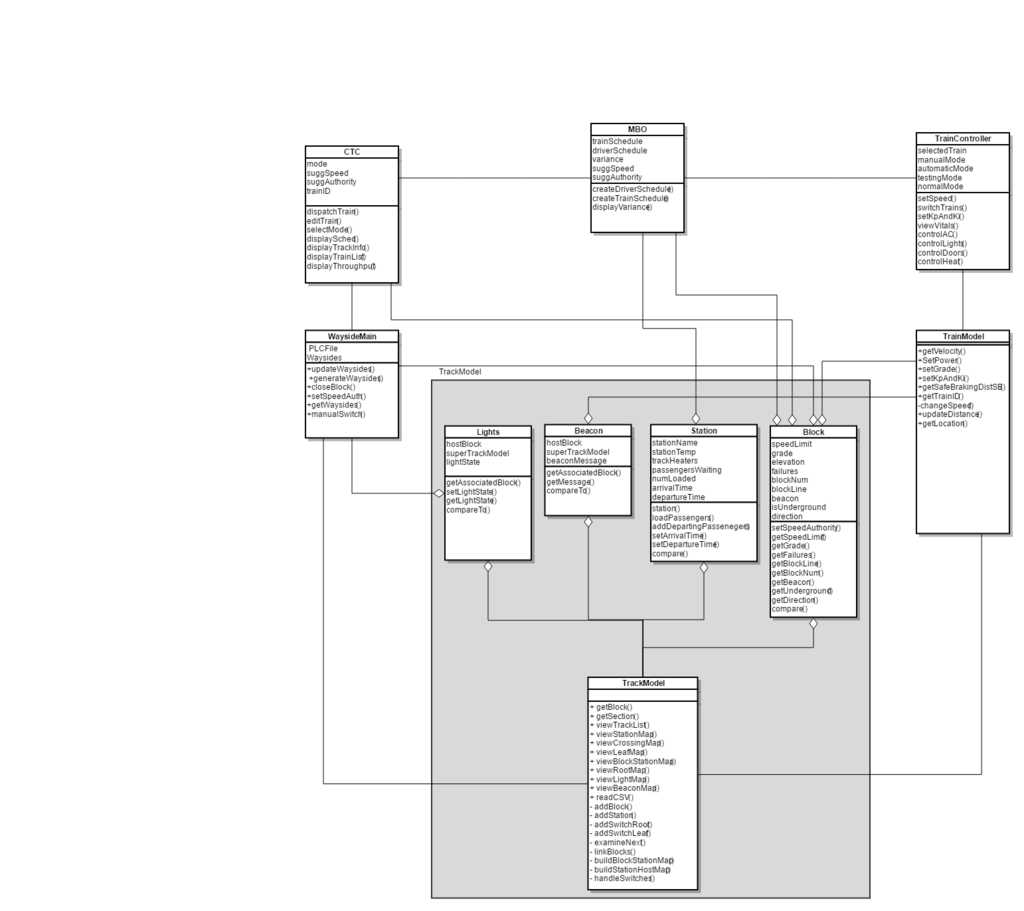
\includegraphics[width=\textwidth]{overallsystem.png}
	\caption{System architecture Diagram}
\end{figure}


In this section, we detail the use cases of each subsystem. The use case of each subsystem is accompanied by brief descriptions of the use cases.

\subsection{Track Model}
In this subsection, the use cases of the train model are provided.

\begin{figure}[H]
	\centering
	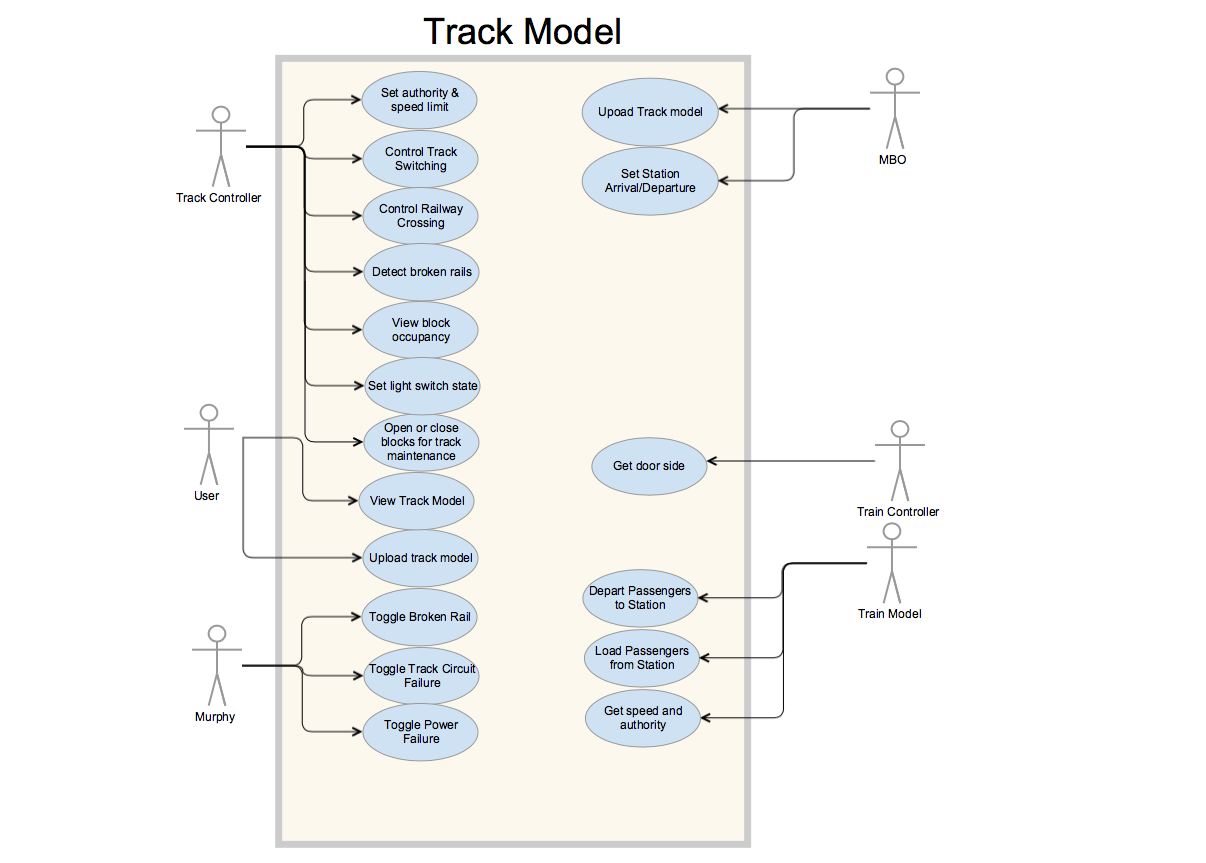
\includegraphics[width=\textwidth]{trackmodelusecase.png}
	\caption{Track model use case diagram}
\end{figure}
   \begin{table}[H]
   	\centering
   	\caption{Set Speed and Authority}
   	\begin{tabular}{|l|l|}
   		\hline
   		Actors & \parbox[t]{10cm}{Track Controller} \\ \hline
   		Description & \parbox[t]{10cm}{The track controller shall be capable of setting a speed and authority via the track circuit modeled by the track model} \\ \hline
   		Data &  \parbox[t]{10cm}{Speed and authority for the trains} \\ \hline
   		Stimulus &  \parbox[t]{10cm}{None. The speed and authority are set externally } \\ \hline
   		Response & \parbox[t]{10cm}{The track model possesses the attributes set.}\\ \hline
   		Comments & \parbox[t]{10cm}{ The track model only exists as a passthrough for this information }  \\ \hline
   	\end{tabular}
   \end{table}
   
   \begin{table}[H]
   	\centering
   	\caption{Set Switch State}
   	\begin{tabular}{|l|l|}
   		\hline
   		Actors & \parbox[t]{10cm}{Track Controller} \\ \hline
   		Description & \parbox[t]{10cm}{The track controller shall be capable of setting the switch of a given state} \\ \hline
   		Data &  \parbox[t]{10cm}{A boolean statement for the state of a switch} \\ \hline
   		Stimulus &  \parbox[t]{10cm}{The Track Controller signal } \\ \hline
   		Response & \parbox[t]{10cm}{Setting the state of the switch}\\ \hline
   		Comments & \parbox[t]{10cm}{ These are set simultaneously with no delays }  \\ \hline
   	\end{tabular}
   \end{table}
   
   \begin{table}[H]
   	\centering
   	\caption{Control Railway Crossing}
   	\begin{tabular}{|l|l|}
   		\hline
   		\hline
   		Actors & \parbox[t]{10cm}{Track Controller} \\ \hline
   		Description & \parbox[t]{10cm}{The track controller shall be capable of setting the railway crossing to a given state} \\ \hline
   		Data &  \parbox[t]{10cm}{A boolean statement for the state of a railway crossing} \\ \hline
   		Stimulus &  \parbox[t]{10cm}{The Track Controller boolean signal } \\ \hline
   		Response & \parbox[t]{10cm}{Setting the state of the railway crossing}\\ \hline
   		Comments & \parbox[t]{10cm}{ These are set simultaneously with no delays }  \\ \hline
   	\end{tabular}
   \end{table}
   
   \begin{table}[H]
   	\centering
   	\caption{Detect Broken Rails}
   	\begin{tabular}{|l|l|}
   		\hline
   		Actors & \parbox[t]{10cm}{Track Controller} \\ \hline
   		Description & \parbox[t]{10cm}{The track controller shall be capable of detecting broken rails} \\ \hline
   		Data &  \parbox[t]{10cm}{A boolean statement for the state of a block} \\ \hline
   		Stimulus &  \parbox[t]{10cm}{A track controller query } \\ \hline
   		Response & \parbox[t]{10cm}{A return of the boolean broken state of the blocks on a track }\\ \hline
   		Comments & \parbox[t]{10cm}{ The track controller calls the track model in this case}  \\ \hline
   	\end{tabular}
   \end{table}
   
   \begin{table}[H]
   	\centering
   	\caption{View Block Occupancy}
   	\begin{tabular}{|l|l|}
   		\hline
   		Actors & \parbox[t]{10cm}{Track Controller} \\ \hline
   		Description & \parbox[t]{10cm}{The track controller shall be capable of viewing block occupancy} \\ \hline
   		Data &  \parbox[t]{10cm}{A boolean statement for the occupancy of the block} \\ \hline
   		Stimulus &  \parbox[t]{10cm}{A track controller query } \\ \hline
   		Response & \parbox[t]{10cm}{A return of the boolean occupied state of the blocks on a trackl }\\ \hline
   		Comments & \parbox[t]{10cm}{ The track controller calls the track model in this case}  \\ \hline
   	\end{tabular}
   \end{table}
   
   \begin{table}[H]
   	\centering
   	\caption{Set Light Switch State}
   	\begin{tabular}{|l|l|}
   		\hline
   		Actors & \parbox[t]{10cm}{Track Controller} \\ \hline
   		Description & \parbox[t]{10cm}{The track controller shall be capable of setting the light states} \\ \hline
   		Data &  \parbox[t]{10cm}{A boolean statement for the next light switch state} \\ \hline
   		Stimulus &  \parbox[t]{10cm}{A track controller function call } \\ \hline
   		Response & \parbox[t]{10cm}{A setting of the light switch state to that set by the track controller }\\ \hline
   		Comments & \parbox[t]{10cm}{ }  \\ \hline
   	\end{tabular}
   \end{table}
   
   \begin{table}[H]
   	\centering
   	\caption{Set Light Switch State}
   	\begin{tabular}{|l|l|}
   		\hline
   		Actors & \parbox[t]{10cm}{Track Controller} \\ \hline
   		Description & \parbox[t]{10cm}{The track controller shall be opening or closing a given block for maintenance} \\ \hline
   		Data &  \parbox[t]{10cm}{A boolean statement for if a given block is open or closed due to maintenance} \\ \hline
   		Stimulus &  \parbox[t]{10cm}{A track controller function call with a boolean variable } \\ \hline
   		Response & \parbox[t]{10cm}{A setting of the blocks open state }\\ \hline
   		Comments & \parbox[t]{10cm}{ This block will not be considered "open" for planning purposes in new path. This is reflected in the nextBlock functionality}  \\ \hline
   	\end{tabular}
   \end{table}
   
   \begin{table}[H]
   	\centering
   	\caption{Upload Track Model}
   	\begin{tabular}{|l|l|}
   		\hline
   		Actors & \parbox[t]{10cm}{User} \\ \hline
   		Description & \parbox[t]{10cm}{The user shall be capable of uploading track models to the track model} \\ \hline
   		Data &  \parbox[t]{10cm}{The track model given in a .csv form. This may be provided by Excel "save as" function or similar.} \\ \hline
   		Stimulus &  \parbox[t]{10cm}{None} \\ \hline
   		Response & \parbox[t]{10cm}{The user loads the files in }\\ \hline
   		Comments & \parbox[t]{10cm}{This will require multiple csv files in practice }  \\ \hline
   	\end{tabular}
   \end{table}
   \begin{table}[H]
   	\centering
   	\caption{Set Light Switch State}
   	\begin{tabular}{|l|l|}
   		\hline
   		Actors & \parbox[t]{10cm}{Track Controller} \\ \hline
   		Description & \parbox[t]{10cm}{The track controller shall be capable of setting the light states} \\ \hline
   		Data &  \parbox[t]{10cm}{A boolean statement for the next light switch state} \\ \hline
   		Stimulus &  \parbox[t]{10cm}{A track controller function call } \\ \hline
   		Response & \parbox[t]{10cm}{A setting of the light switch state to that set by the track controller }\\ \hline
   		Comments & \parbox[t]{10cm}{ }  \\ \hline
   	\end{tabular}
   \end{table}
   
   \begin{table}[H]
   	\centering
   	\caption{Toggle Broken Rail}
   	\begin{tabular}{|l|l|}
   		\hline
   		Actors & \parbox[t]{10cm}{Murphy} \\ \hline
   		Description & \parbox[t]{10cm}{A test environment shall be provided to toggle the rail broken state for testing} \\ \hline
   		Data &  \parbox[t]{10cm}{A boolean statement to set the rail to} \\ \hline
   		Stimulus &  \parbox[t]{10cm}{External user testing stimulus} \\ \hline
   		Response & \parbox[t]{10cm}{Setting a given block to broken or fixed}\\ \hline
   		Comments & \parbox[t]{10cm}{ This should be considered for test purposes of other modules}  \\ \hline
   	\end{tabular}
   \end{table}
   
   \begin{table}[H]
   	\centering
   	\caption{Toggle Track Circuit Failure}
   	\begin{tabular}{|l|l|}
   		\hline
   		Actors & \parbox[t]{10cm}{Murphy} \\ \hline
   		Description & \parbox[t]{10cm}{A test environment shall be provided to toggle the circuit failure state for testing} \\ \hline
   		Data &  \parbox[t]{10cm}{A boolean statement to set the track circuit functionality} \\ \hline
   		Stimulus &  \parbox[t]{10cm}{External user testing stimulus} \\ \hline
   		Response & \parbox[t]{10cm}{Setting the track circuit to broken or functional}\\ \hline
   		Comments & \parbox[t]{10cm}{ This should be considered for test purposes of other modules}  \\ \hline
   	\end{tabular}
   \end{table}
   
   \begin{table}[H]
   	\centering
   	\caption{Toggle Power Failure}
   	\begin{tabular}{|l|l|}
   		\hline
   		Actors & \parbox[t]{10cm}{Murphy} \\ \hline
   		Description & \parbox[t]{10cm}{A test environment shall be provided to toggle the power failure state for testing} \\ \hline
   		Data &  \parbox[t]{10cm}{A boolean statement to set the power failure state of a rail to} \\ \hline
   		Stimulus &  \parbox[t]{10cm}{External user testing stimulus} \\ \hline
   		Response & \parbox[t]{10cm}{Setting a broken or fixed power state to}\\ \hline
   		Comments & \parbox[t]{10cm}{ This should be considered for test purposes of other modules}  \\ \hline
   	\end{tabular}
   \end{table}
   
   \begin{table}[H]
   	\centering
   	\caption{Upload Track Module}
   	\begin{tabular}{|l|l|}
   		\hline
   		Actors & \parbox[t]{10cm}{MBO} \\ \hline
   		Description & \parbox[t]{10cm}{Upload a track model to the track module} \\ \hline
   		Data &  \parbox[t]{10cm}{identical to the user inputs} \\ \hline
   		Stimulus &  \parbox[t]{10cm}{Initialization of a program} \\ \hline
   		Response & \parbox[t]{10cm}{The reading of the excel file}\\ \hline
   		Comments & \parbox[t]{10cm}{Functionally equivalent to the read track info for the user}  \\ \hline
   	\end{tabular}
   \end{table}
	 \begin{table}[H]
	 	\centering
	 	\caption{Set Station Arrival/Departure}
	 	\begin{tabular}{|l|l|}
	 		\hline
	 		Actors & \parbox[t]{10cm}{MBO} \\ \hline
	 		Description & \parbox[t]{10cm}{Set station arrival and departure time} \\ \hline
	 		Data &  \parbox[t]{10cm}{Receives the expected arrival and departure time from the MBO and displays them at a station} \\ \hline
	 		Stimulus &  \parbox[t]{10cm}{The MBO setting an arrival or departure at a given station} \\ \hline
	 		Response & \parbox[t]{10cm}{Setting an arrival or departure at a given station}\\ \hline
	 		Comments & \parbox[t]{10cm}{Set and called by the MBO}  \\ \hline
	 	\end{tabular}
	 \end{table}
	  \begin{table}[H]
	  	\centering
	  	\caption{Get Door Side}
	  	\begin{tabular}{|l|l|}
	  		\hline
	  		Actors & \parbox[t]{10cm}{Train Controller} \\ \hline
	  		Description & \parbox[t]{10cm}{Get the side of the door for arrival at a station given the visible beacon} \\ \hline
	  		Data &  \parbox[t]{10cm}{Returns the side of the door to open for a given train} \\ \hline
	  		Stimulus &  \parbox[t]{10cm}{Query with a station given a beacon} \\ \hline
	  		Response & \parbox[t]{10cm}{Side of the train to open the door on}\\ \hline
	  		Comments & \parbox[t]{10cm}{Set and called by the Train Conroller}  \\ \hline
	  	\end{tabular}
	  \end{table}
	  
	  \begin{table}[H]
	  	\centering
	  	\caption{Depart Passengers to Station}
	  	\begin{tabular}{|l|l|}
	  		\hline
	  		Actors & \parbox[t]{10cm}{Train Model} \\ \hline
		   	Description & \parbox[t]{10cm}{Depart passengers from a train to a station} \\ \hline
	  		Data &  \parbox[t]{10cm}{Number of passengers to depart} \\ \hline
	  		Stimulus &  \parbox[t]{10cm}{Train model calling the station of the track model} \\ \hline
	  		Response & \parbox[t]{10cm}{Add the people to the station loitering group}\\ \hline
	  		Comments & \parbox[t]{10cm}{Set and called by the Train Model}  \\ \hline
	  	\end{tabular}
	  \end{table}
	  
	  \begin{table}[H]
	  	\centering
	  	\caption{Get speed and authority from a given block}
	  	\begin{tabular}{|l|l|}
	  		\hline
	  		Actors & \parbox[t]{10cm}{Train Model} \\ \hline
	  		Description & \parbox[t]{10cm}{Calls a given block} \\ \hline
	  		Data &  \parbox[t]{10cm}{Number of passengers to depart} \\ \hline
	  		Stimulus &  \parbox[t]{10cm}{Train model calling the station of the track model} \\ \hline
	  		Response & \parbox[t]{10cm}{Return speed and authority at a given block}\\ \hline
	  		Comments & \parbox[t]{10cm}{Set and called by the Train Model}  \\ \hline
	  	\end{tabular}
	  \end{table}
	  
	  \begin{table}[H]
	  	\centering
	  	\caption{Load Passengers From Station}
	  	\begin{tabular}{|l|l|}
	  		\hline
	  		Actors & \parbox[t]{10cm}{Train Controller} \\ \hline
	  		Description & \parbox[t]{10cm}{Load passengers to a track model from a station} \\ \hline
	  		Data &  \parbox[t]{10cm}{Maximum number of passengers to load a train to capacity} \\ \hline
	  		Stimulus &  \parbox[t]{10cm}{Train model queryiing the track model} \\ \hline
	  		Response & \parbox[t]{10cm}{Number of people to add to the train}\\ \hline
	  		Comments & \parbox[t]{10cm}{Set and called by the Train Controller}  \\ \hline
	  	\end{tabular}
	  \end{table}
	  
\subsection{Track Controller}
In this subsection, the use cases of the track controller are provided.

\begin{figure}[H]
	\centering
	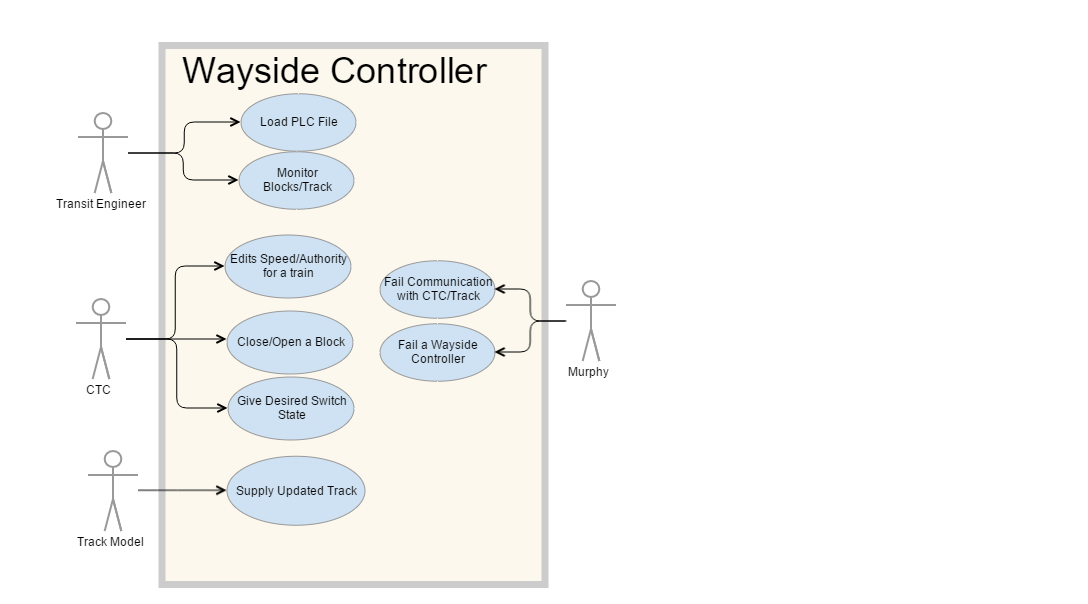
\includegraphics[scale=.5]{trackcontrollerusecase.png}
	\caption{Track controller use case diagram}
\end{figure}
\begin{table}[H]
	\centering
	\caption{Load PLC File}
	\begin{tabular}{|l|l|}
		\hline
		Actors & \parbox[t]{10cm}{Transit Engineer, Wayside Controller} \\ \hline
		Description & \parbox[t]{10cm}{A Transit Engineer will load a PLC file upon startup of the Wayside unit(s), and will do so by either browsing for a file or supplying the file path.} \\ \hline
		Data &  \parbox[t]{10cm}{PLC File's name, path} \\ \hline
		Stimulus &  \parbox[t]{10cm}{ 'Load' button pressed} \\ \hline
		Response & \parbox[t]{10cm}{Validity of File checked; Invalid File/Success of Load will be displayed to Transit Engineer}\\ \hline
		Comments & \parbox[t]{10cm}{Proper formatting/convention of PLC file is required	}  \\ \hline
	\end{tabular}
\end{table}

\begin{table}[H]
	\centering
	\caption{Monitor Blocks/Track}
	\begin{tabular}{|l|l|}
		\hline
		Actors & \parbox[t]{10cm}{Transit Engineer, Wayside Controller} \\ \hline
		Description & \parbox[t]{10cm}{For a given wayside, a Transit Engineer may select a block (by Line, Section, Block) from dropdowns to view its characteristics i.e. switch state \& crossing status (if applicable), occupancy, lights} \\ \hline
		Data &  \parbox[t]{10cm}{Track Blocks, Switches, Crossings, Lights} \\ \hline
		Stimulus &  \parbox[t]{10cm}{Block selected} \\ \hline
		Response & \parbox[t]{10cm}{Information queried from block and displayed}\\ \hline
		Comments & \parbox[t]{10cm}{Selection of blocks changes based on Wayside Controller selected}  \\ \hline
	\end{tabular}
\end{table}

\begin{table}[H]
	\centering
	\caption{Dispatch/Edit Train}
	\begin{tabular}{|l|l|}
		\hline
		Actors & \parbox[t]{10cm}{CTC, Wayside Controller} \\ \hline
		Description & \parbox[t]{10cm}{A CTC will dispatch a train/update a train with a given speed and authority (passed to wayside controller) which will then be relayed to the track model by the wayside controller.} \\ \hline
		Data &  \parbox[t]{10cm}{Speed, Authority, Block} \\ \hline
		Stimulus &  \parbox[t]{10cm}{Speed, Authority, and Block passed to Wayside Controller} \\ \hline
		Response & \parbox[t]{10cm}{Wayside sets Speed, Authority of given block on the track model}\\ \hline
		Comments & \parbox[t]{10cm}{}  \\ \hline
	\end{tabular}
\end{table}

\begin{table}[H]
	\centering
	\caption{Open/Close a Block}
	\begin{tabular}{|l|l|}
		\hline
		Actors & \parbox[t]{10cm}{CTC, Wayside Controller} \\ \hline
		Description & \parbox[t]{10cm}{The CTC will prompt the Wayside to close or open a block for maintenance.} \\ \hline
		Data &  \parbox[t]{10cm}{Block, Open/Closed Status} \\ \hline
		Stimulus &  \parbox[t]{10cm}{CTC prompts Wayside controller to close or open a block.} \\ \hline
		Response & \parbox[t]{10cm}{Wayside sets status of given Block to open/closed.}\\ \hline
		Comments & \parbox[t]{10cm}{}  \\ \hline
	\end{tabular}
\end{table}

\begin{table}[H]
	\centering
	\caption{Supply Updated Track}
	\begin{tabular}{|l|l|}
		\hline
		Actors & \parbox[t]{10cm}{Track Model, Wayside Controller} \\ \hline
		Description & \parbox[t]{10cm}{The Track Model will provide Block Occupancies, Switch statuses, and Crossing statuses to the Wayside Controller} \\ \hline
		Data &  \parbox[t]{10cm}{Block, Switch, Crossing} \\ \hline
		Stimulus &  \parbox[t]{10cm}{Track sends updated information} \\ \hline
		Response & \parbox[t]{10cm}{Wayside gives updated info to PLC code}\\ \hline
		Comments & \parbox[t]{10cm}{}  \\ \hline
	\end{tabular}
\end{table}

\begin{table}[H]
	\centering
	\caption{Fail Communication with CTC/Track Model}
	\begin{tabular}{|l|l|}
		\hline
		Actors & \parbox[t]{10cm}{Murphy, Wayside Controller} \\ \hline
		Description & \parbox[t]{10cm}{Murphy will eliminate communication between the Wayside Controller and the CTC and Track.} \\ \hline
		Data &  \parbox[t]{10cm}{N/A} \\ \hline
		Stimulus &  \parbox[t]{10cm}{ 'Communication Fail' button pressed} \\ \hline
		Response & \parbox[t]{10cm}{All Trains are stopped.}\\ \hline
		Comments & \parbox[t]{10cm}{}  \\ \hline
	\end{tabular}
\end{table}

\begin{table}[H]
	\centering
	\caption{Fail a Wayside}
	\begin{tabular}{|l|l|}
		\hline
		Actors & \parbox[t]{10cm}{Murphy, Wayside Controller} \\ \hline
		Description & \parbox[t]{10cm}{Murphy will break a Wayside Controller causing the unit to be non-responsive} \\ \hline
		Data &  \parbox[t]{10cm}{N/A} \\ \hline
		Stimulus &  \parbox[t]{10cm}{ 'Fail Wayside' button pressed} \\ \hline
		Response & \parbox[t]{10cm}{All trains within jurisdiction of Wayside's line are stopped.}\\ \hline
		Comments & \parbox[t]{10cm}{i.e. Red Line can operate if Green Line is shut down.}  \\ \hline
	\end{tabular}
\end{table}
\subsection{Train Model}
In this subsection, the use cases of the train model are provided.

\begin{figure}[H]
	\centering
	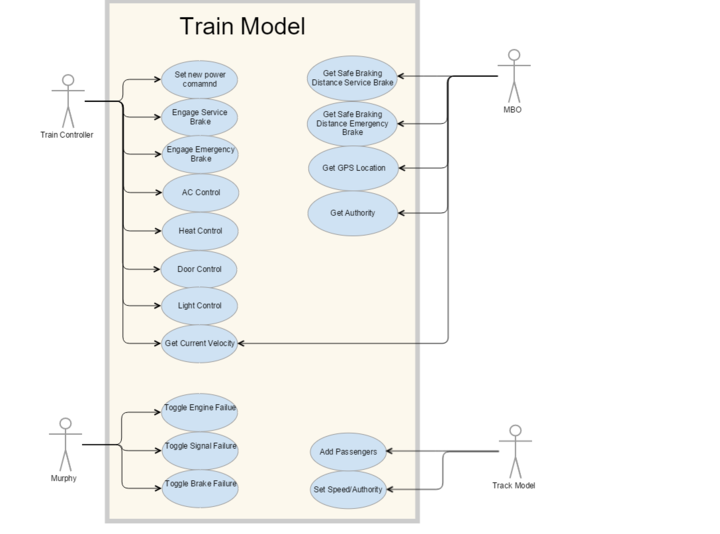
\includegraphics[scale=.5]{trainmodelusecase.png}
	\caption{Train model use case diagram}
\end{figure}
   
   \begin{table}[H]
   	\centering
   	\caption{Set New Power Command}
   	\begin{tabular}{|l|l|}
   		\hline
   		Actors & \parbox[t]{10cm}{Train Controller} \\ \hline
   		Description & \parbox[t]{10cm}{Train Controller will set a new power command based on the current velocity of the train and the new setpoint speed set by the driver. This power command will be used to determine the force applied to the train and thus compute the new current velocity.} \\ \hline
   		Data &  \parbox[t]{10cm}{Power Command issued to the train} \\ \hline
   		Stimulus &  \parbox[t]{10cm}{When a setpoint speed is provided to the train controller, a Power command is computed using the current velocity and sent to train} \\ \hline
   		Response & \parbox[t]{10cm}{New current velocity is returned to actor at the end of the computation. }\\ \hline
   		Comments & \parbox[t]{10cm}{ }  \\ \hline
   	\end{tabular}
   \end{table}
   
   \begin{table}[H]
   	\centering
   	\caption{Engage Service Brake}
   	\begin{tabular}{|l|l|}
   		\hline
   		Actors & \parbox[t]{10cm}{Train Controller} \\ \hline
   		Description & \parbox[t]{10cm}{Train controller will engage or disengage the service brake in order to slow down or stop the train for any given reason. Once engaged the power command will be set to zero and the train will begin to decelerate } \\ \hline
   		Data &  \parbox[t]{10cm}{Service Brake command } \\ \hline
   		Stimulus &  \parbox[t]{10cm}{Service brake will be engaged under the following conditions:\\1) Service brake button is manually pressed by the driver via the train controller\\2) Failure occurs in the train that requires the train to stop, this will engage the service brakes unless failure is caused by service brakes\\3) Train is set to slow down and service brakes are applied to reduce speed} \\ \hline
   		Response & \parbox[t]{10cm}{Service brake status is set to engaged and train begins to decelerate at service brake deceleration rate.}\\ \hline
   		Comments & \parbox[t]{10cm}{The service brake can either posses the status of on, off , or failure.}  \\ \hline
   	\end{tabular}
   \end{table}
   
   \begin{table}[H]
   	\centering
   	\caption{Engage Emergency Brake	}
   	\begin{tabular}{|l|l|}
   		\hline
   		Actors & \parbox[t]{10cm}{Train Controller} \\ \hline
   		Description & \parbox[t]{10cm}{Train controller will engage or disengage the emergency brake in order to slow down or stop the train for any emergencies that may occur. Once engaged the power command will be set to zero and the train will begin to decelerate } \\ \hline
   		Data &  \parbox[t]{10cm}{Emergency Brake command } \\ \hline
   		Stimulus &  \parbox[t]{10cm}{Emergency brake will be engaged under the following conditions:\\1) Emergency brake button is manually pressed by the driver or passenger via the train controller\\2) Failure occurs in the service brakes and the emergency brakes are required to stop the train  } \\ \hline
   		Response & \parbox[t]{10cm}{Emergency brake status is set to engaged and train begins to decelerate at emergency brake deceleration rate.}\\ \hline
   		Comments & \parbox[t]{10cm}{The Emergency brake can either posses the status of on or off. For this model we are assuming that the emergency brakes never fail}  \\ \hline
   	\end{tabular}
   \end{table}
   
   
   \begin{table}[H]
   	\centering
   	\caption{Air Conditioning (AC) Control}
   	\begin{tabular}{|l|l|}
   		\hline
   		Actors & \parbox[t]{10cm}{Train Controller} \\ \hline
   		Description & \parbox[t]{10cm}{Train controller will activate or deactivate the Air conditioning unit onboard the train to decrease the current temperature of the train.} \\ \hline
   		Data &  \parbox[t]{10cm}{Air conditioning command  } \\ \hline
   		Stimulus &  \parbox[t]{10cm}{The air conditioning will be turned on or off by the train controller. This will either be performed manually by the driver using a button or automatically by the train controller based on current temperature and thermostat setting.} \\ \hline
   		Response & \parbox[t]{10cm}{AC control set to on will result in a gradual decrease of the current train internal temperature. }\\ \hline
   		Comments & \parbox[t]{10cm}{The AC can either posses the status of on, off, or failure.}  \\ \hline
   	\end{tabular}
   \end{table}
   
   \begin{table}[H]
   	\centering
   	\caption{Heater Control}
   	\begin{tabular}{|l|l|}
   		\hline
   		Actors & \parbox[t]{10cm}{Train Controller} \\ \hline
   		Description & \parbox[t]{10cm}{Train controller will activate or deactivate the heating unit onboard the train to increase the current temperature of the train.} \\ \hline
   		Data &  \parbox[t]{10cm}{Heater command } \\ \hline
   		Stimulus &  \parbox[t]{10cm}{The heating unit will be turned on or off by the train controller. This will either be performed manually by the driver using a button or automatically by the train controller based on current temperature and thermostat setting.} \\ \hline
   		Response & \parbox[t]{10cm}{Heater control set to on will result in a gradual increase of the current train internal temperature. }\\ \hline
   		Comments & \parbox[t]{10cm}{The heater can either posses the status of on, off, or failure. }  \\ \hline
   	\end{tabular}
   \end{table}
   
   \begin{table}[H]
   	\centering
   	\caption{Door Control}
   	\begin{tabular}{|l|l|}
   		\hline
   		Actors & \parbox[t]{10cm}{Train Controller} \\ \hline
   		Description & \parbox[t]{10cm}{Train controller will open and close the doors on the left and right side individually using individual commands for each side. } \\ \hline
   		Data &  \parbox[t]{10cm}{Left door command, Right door command } \\ \hline
   		Stimulus &  \parbox[t]{10cm}{The left or right doors will be opened or closed by the train controller. This will either be performed manually by the driver using a button or automatically by the train controller upon arrival and departure at each station.} \\ \hline
   		Response & \parbox[t]{10cm}{If the right door command is passed, all doors on the right side are opened. If the left door command is passed, all doors on the left side are opened. }\\ \hline
   		Comments & \parbox[t]{10cm}{The Left and Right doors can either posses the status of open, closed, or failure.}  \\ \hline
   	\end{tabular}
   \end{table}
   
   \begin{table}[H]
   	\centering
   	\caption{Light Control}
   	\begin{tabular}{|l|l|}
   		\hline
   		Actors & \parbox[t]{10cm}{Train Controller} \\ \hline
   		Description & \parbox[t]{10cm}{Train controller will turn the interior lights onboard the train on and off based on time of day and location of train (e.g. within tunnel or not)} \\ \hline
   		Data &  \parbox[t]{10cm}{Interior Light command } \\ \hline
   		Stimulus &  \parbox[t]{10cm}{The lights will be toggled on and off by the train controller. This will either be performed manually by the driver using a button or automatically by the train controller based on time of day and upon entering and exiting a tunnel} \\ \hline
   		Response & \parbox[t]{10cm}{If the light command is passed, all lights onboard the train are turned on.}\\ \hline
   		Comments & \parbox[t]{10cm}{The interior lights can either posses the status of on, off, or failure. }  \\ \hline
   	\end{tabular}
   \end{table}
   
   \begin{table}[H]
   	\centering
   	\caption{Get Current Velocity}
   	\begin{tabular}{|l|l|}
   		\hline
   		Actors & \parbox[t]{10cm}{Train Controller, MBO} \\ \hline
   		Description & \parbox[t]{10cm}{A call will be made to request the current velocity of the train and this will be passed back to the actor which required it. The train controllor will request the current velocity in order to compute the power command to send to the train model. The MBO will request the current velocity in order to compute the variation between the suggested speed and the actual speed of the train.} \\ \hline
   		Data &  \parbox[t]{10cm}{Current Velocity value} \\ \hline
   		Stimulus &  \parbox[t]{10cm}{A request will be sent to the train model to obtain the current velocity of the train at that given moment} \\ \hline
   		Response & \parbox[t]{10cm}{The current velocity of the train will be returned to the caller in MPH.}\\ \hline
   		Comments & \parbox[t]{10cm}{ }  \\ \hline
   	\end{tabular}
   \end{table}
   
   \begin{table}[H]
   	\centering
   	\caption{Toggle Engine Failure}
   	\begin{tabular}{|l|l|}
   		\hline
   		Actors & \parbox[t]{10cm}{Murphy} \\ \hline
   		Description & \parbox[t]{10cm}{Murphy is able to toggle the engine failure status in order to distrupt the train's engine. Once engaged the train will be required to stop until the issue is resolved.} \\ \hline
   		Data &  \parbox[t]{10cm}{Engine Failure command} \\ \hline
   		Stimulus &  \parbox[t]{10cm}{A command will be sent to the train model from the Murphy console to toggle the failure status of the train's engine.} \\ \hline
   		Response & \parbox[t]{10cm}{The engine failure status will be toggled as a response to the command. When an engine failure occurs the service brakes are also engaged to bring the train to a stop until issues are resolved.}\\ \hline
   		Comments & \parbox[t]{10cm}{The engine failure status will toggle between failure, and non-failure. }  \\ \hline
   	\end{tabular}
   \end{table}
   
   \begin{table}[H]
   	\centering
   	\caption{Toggle Signal Failure}
   	\begin{tabular}{|l|l|}
   		\hline
   		Actors & \parbox[t]{10cm}{Murphy} \\ \hline
   		Description & \parbox[t]{10cm}{Murphy is able to toggle the signal failure status in order to distrupt the train's signaling and communication abilities. Once engaged the train will be required to stop until the issue is resolved.} \\ \hline
   		Data &  \parbox[t]{10cm}{Signal Failure command} \\ \hline
   		Stimulus &  \parbox[t]{10cm}{A command will be sent to the train model from the Murphy console to toggle the failure status of the train's signaling system.} \\ \hline
   		Response & \parbox[t]{10cm}{The signal failure status will be toggled as a response to the command. When a signal failure occurs the service brakes are also engaged to bring the train to a stop until issues are resolved.}\\ \hline
   		Comments & \parbox[t]{10cm}{The signal failure status will toggle between failure, and non-failure.}  \\ \hline
   	\end{tabular}
   \end{table}
   
   \begin{table}[H]
   	\centering
   	\caption{Toggle Brake Failure}
   	\begin{tabular}{|l|l|}
   		\hline
   		Actors & \parbox[t]{10cm}{Murphy} \\ \hline
   		Description & \parbox[t]{10cm}{Murphy is able to toggle the brake failure status in order to distrupt the train's service brake. Once engaged the train will be required to stop until the issue is resolved.} \\ \hline
   		Data &  \parbox[t]{10cm}{Brake Failure command} \\ \hline
   		Stimulus &  \parbox[t]{10cm}{A command will be sent to the train model from the Murphy console to toggle the failure status of the train's service brake} \\ \hline
   		Response & \parbox[t]{10cm}{The brake failure status will be toggled as a response to the command. When a service brake failure occurs the emergency brakes are also engaged to bring the train to a stop until issues are resolved.}\\ \hline
   		Comments & \parbox[t]{10cm}{The brake failure status will toggle between failure, and non-failure.}  \\ \hline
   	\end{tabular}
   \end{table}
   
   \begin{table}[H]
   	\centering
   	\caption{Get Safe Braking Distance (Service Brake)}
   	\begin{tabular}{|l|l|}
   		\hline
   		Actors & \parbox[t]{10cm}{MBO} \\ \hline
   		Description & \parbox[t]{10cm}{In order to better determine the train's footprint the MBO will call to obtain the safe braking distance of the Train. This will be the distance required to bring the train to a complete stop using the service brake deceleration rate. This distance will vary based on the number of passengers on board the train and the current velocity of the train.} \\ \hline
   		Data &  \parbox[t]{10cm}{Safe Braking Distance for Service Brake} \\ \hline
   		Stimulus &  \parbox[t]{10cm}{Command will be requested from the MBO to get the current safe braking distance using the service brakes which would be computed based on the current velocity and mass of the train.} \\ \hline
   		Response & \parbox[t]{10cm}{The safe braking distance using the service brakes will be returned to the MBO.}\\ \hline
   		Comments & \parbox[t]{10cm}{ }  \\ \hline
   	\end{tabular}
   \end{table}
   
   \begin{table}[H]
   	\centering
   	\caption{Get Safe Braking Distance (Emergency Brake)}
   	\begin{tabular}{|l|l|}
   		\hline
   		Actors & \parbox[t]{10cm}{MBO} \\ \hline
   		Description & \parbox[t]{10cm}{In order to better determine the train's footprint the MBO will call to obtain the safe braking distance of the Train. This will be the distance required to bring the train to a complete stop using the emergency brake deceleration rate. This distance will vary based on the number of passengers on board the train and the current velocity of the train.} \\ \hline
   		Data &  \parbox[t]{10cm}{Safe Braking Distance for Emergency Brake} \\ \hline
   		Stimulus &  \parbox[t]{10cm}{Command will be requested from the MBO to get the current safe braking distance using the emergency brakes which would be computed based on the current velocity and mass of the train.} \\ \hline
   		Response & \parbox[t]{10cm}{The safe braking distance using the emergency brakes will be returned to the MBO.}\\ \hline
   		Comments & \parbox[t]{10cm}{ }  \\ \hline
   	\end{tabular}
   \end{table}
   
   \begin{table}[H]
   	\centering
   	\caption{Get GPS Location}
   	\begin{tabular}{|l|l|}
   		\hline
   		Actors & \parbox[t]{10cm}{MBO} \\ \hline
   		Description & \parbox[t]{10cm}{The MBO will elect to receive the current GPS location to determine the train's current location to the nearest meter. This will be determined by calculating the distance traveled by the train and compute the distance into the current block to return to the MBO} \\ \hline
   		Data &  \parbox[t]{10cm}{Current Block, Distance Into block} \\ \hline
   		Stimulus &  \parbox[t]{10cm}{Command will be requested from the MBO to get the current GPS location from the train} \\ \hline
   		Response & \parbox[t]{10cm}{GPS location will be returned providing the current block the train is in as well as the distance into that current block to the nearest meter.}\\ \hline
   		Comments & \parbox[t]{10cm}{ }  \\ \hline
   	\end{tabular}
   \end{table}
   
   \begin{table}[H]
   	\centering
   	\caption{Get Authority}
   	\begin{tabular}{|l|l|}
   		\hline
   		Actors & \parbox[t]{10cm}{MBO} \\ \hline
   		Description & \parbox[t]{10cm}{The MBO will request to receive the current Authority of the given train. This will be used in conjuction with the suggested authority to determine the variation between suggested authority and actual authority for the train.} \\ \hline
   		Data &  \parbox[t]{10cm}{Current Authority} \\ \hline
   		Stimulus &  \parbox[t]{10cm}{Command will be requested from the MBO to get the current Authority from the train} \\ \hline
   		Response & \parbox[t]{10cm}{Current authority will be returned for that given train}\\ \hline
   		Comments & \parbox[t]{10cm}{ }  \\ \hline
   	\end{tabular}
   \end{table}
   
   \begin{table}[H]
   	\centering
   	\caption{Add Passengers}
   	\begin{tabular}{|l|l|}
   		\hline
   		Actors & \parbox[t]{10cm}{Track Model} \\ \hline
   		Description & \parbox[t]{10cm}{The track model will randomly generate a number of passengers to wait at a station then upon arrival to a station a random number of passengers will board based on space avaliable on the train. This number will be sent to the train model to modify passenger count and mass of train based on capacity.} \\ \hline
   		Data &  \parbox[t]{10cm}{ Number of passengers boarding} \\ \hline
   		Stimulus &  \parbox[t]{10cm}{Command will be requested from the MBO to get the current Authority from the train} \\ \hline
   		Response & \parbox[t]{10cm}{Based on space on board, a random number of passengers between 0 and amount of space will be passed to the train model}\\ \hline
   		Comments & \parbox[t]{10cm}{ }  \\ \hline
   	\end{tabular}
   \end{table}
   
   \begin{table}[H]
   	\centering
   	\caption{Set Speed/ Authority}
   	\begin{tabular}{|l|l|}
   		\hline
   		Actors & \parbox[t]{10cm}{Track Model} \\ \hline
   		Description & \parbox[t]{10cm}{The track model will pass the speed and authority to the train model. This speed and authority will then be passed to the train controller with no variation.} \\ \hline
   		Data &  \parbox[t]{10cm}{ Speed, Authority} \\ \hline
   		Stimulus &  \parbox[t]{10cm}{Command will be sent to train model with speed and authority} \\ \hline
   		Response & \parbox[t]{10cm}{Speed and authority will be passed to train controller.}\\ \hline
   		Comments & \parbox[t]{10cm}{ }  \\ \hline
   	\end{tabular}
   \end{table}
   
   \begin{table}[H]
   	\centering
   	\caption{Set Current Block}
   	\begin{tabular}{|l|l|}
   		\hline
   		Actors & \parbox[t]{10cm}{Track Model} \\ \hline
   		Description & \parbox[t]{10cm}{The track model will pass the current block the train is on as the train enters each new block area. This current block object will provide the train with the block's grade as well as its length, to be used by the train's GPS } \\ \hline
   		Data &  \parbox[t]{10cm}{Current Block} \\ \hline
   		Stimulus &  \parbox[t]{10cm}{Command will be sent to train model with current block } \\ \hline
   		Response & \parbox[t]{10cm}{Block length will be extracted for train GPS, and Block grade will be extracted for train movement calculations}\\ \hline
   		Comments & \parbox[t]{10cm}{ }  \\ \hline
   	\end{tabular}
   \end{table}

\subsection{Train Controller}
In this subsection, the use cases of the train controller are provided.

\begin{figure}[H]
	\centering
	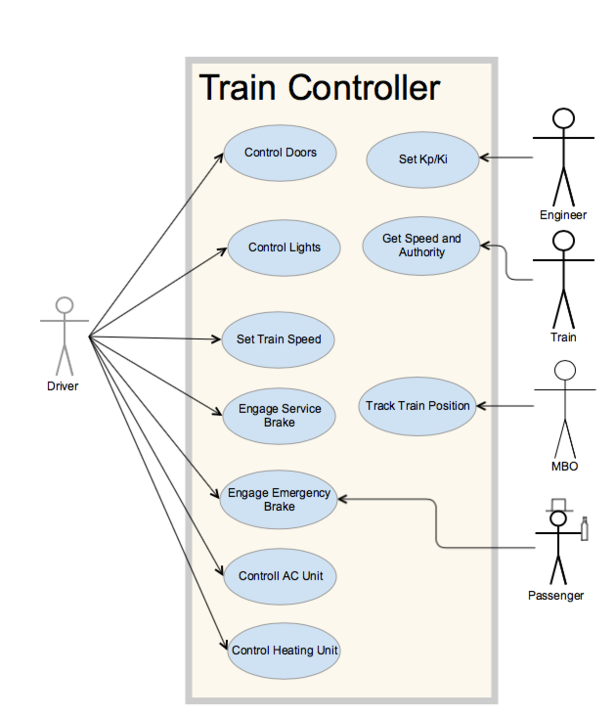
\includegraphics[width=\textwidth]{traincontrollerusecase.png}
	\caption{Train controller use case diagram}
\end{figure}

\begin{table}[H]
	\centering
	\caption{Select Train}
	\begin{tabular}{|l|l|}
		\hline
		Actors & \parbox[t]{10cm}{Driver} \\ \hline
		Description & \parbox[t]{10cm}{The user picks a train from the dropdown and switches the train controlled by the Train Controller to the selected train by clicking the 'Switch' button. The Train Controller then passes the selected train to its sub-components. } \\ \hline
		Data &  \parbox[t]{10cm}{Train ID corresponding to the item in dropdown box.} \\ \hline
		Response & \parbox[t]{10cm}{The Train Controller now controls the train that was picked from the dropdown.  }\\ \hline
		Comments & \parbox[t]{10cm}{}  \\ \hline
	\end{tabular}
\end{table}


   \begin{table}[H]
   	\centering
   	\caption{Set Speed}
   	\begin{tabular}{|l|l|}
   		\hline
   		Actors & \parbox[t]{10cm}{Driver, Train} \\ \hline
   		Description & \parbox[t]{10cm}{Begins the process of changing the selected train's speed by using power control law. The power command is passed to the train and the train changes to a new speed. This continues until the train's speed is equal to the speed set by the driver or system.} \\ \hline
   		Data &  \parbox[t]{10cm}{Set speed, block speed, suggested speed, selected train} \\ \hline
   		Stimulus &  \parbox[t]{10cm}{Happens when th 'Set Speed' button is clicked or the train enters a block with a different block speed and has to adjust. } \\ \hline
   		Response & \parbox[t]{10cm}{Sends a power command to the selected train, signaling to either increases or decreases its speed until the actual speed of the train equals the set speed.  }\\ \hline
   		Comments & \parbox[t]{10cm}{The set speed must not be over the suggested speed or the block speed. This is made sure by the UI elements in the Speed Controller. }  \\ \hline
   	\end{tabular}
   \end{table}
   
  
 \begin{table}[H]
   	\centering
   	\caption{Control Utilities}
   	\begin{tabular}{|l|l|}
   		\hline
   		Actors & \parbox[t]{10cm}{Driver, Train} \\ \hline
   		Description & \parbox[t]{10cm}{The driver will open, close, turn on, or turn off the selected train's utilities such as AC, Heat, Lights, and Left/Right Doors or the utilities will be controlled automatically by the Train Controller. This is done by selecting the corresponding radio button from the Utility Panel. } \\ \hline
   		Data &  \parbox[t]{10cm}{Selected train} \\ \hline
   		Stimulus &  \parbox[t]{10cm}{The user changing the states of the radio button or the system detects that a utility must be turn on, off, opened, or closed.  } \\ \hline
   		Response & \parbox[t]{10cm}{Train updates the states of the corresponding utilities. }\\ \hline
   		Comments & \parbox[t]{10cm}{AC and Heat cannot be on at the same time. This is made sure by the UI elements in the Utility Panel. }  \\ \hline
   	\end{tabular}
   \end{table}
   
\begin{table}[H]
   	\centering
   	\caption{Set $K_{p}$ and $K_{i}$}
   	\begin{tabular}{|l|l|}
   		\hline
   		Actors & \parbox[t]{10cm}{Engineer, Train} \\ \hline
   		Description & \parbox[t]{10cm}{The Engineer will set $K_p$ and $K_i$ of the selected train by inputting the value as double and clicking the 'Set' button.} \\ \hline
   		Data &  \parbox[t]{10cm}{The selected train and doubles representing $K_p$ and $K_i$} \\ \hline
   		Stimulus &  \parbox[t]{10cm}{The selected train has no $K_p$ and $K_i$ set or the user clicks the 'Set $K_p$/$K_i$' button on the Train Controller.} \\ \hline
   		Response & \parbox[t]{10cm}{The $K_p$ and $K_i$ of the train will be set. }\\ \hline
   		Comments & \parbox[t]{10cm}{If the $K_p$ and the $K_i$ are not chosen for a selected train when the train is first selected, a window will pop up to allow the Engineer to set the $K_p$ and $K_i$.}  \\ \hline
   	\end{tabular}
   \end{table}

      \begin{table}[H]
   	\centering
   	\caption{Engage Service Brake}
   	\begin{tabular}{|l|l|}
   		\hline
   		Actors & \parbox[t]{10cm}{Driver, Train} \\ \hline
   		Description & \parbox[t]{10cm}{Initiates the service brake on the selected train, decreasing its speed.} \\ \hline
   		Data &  \parbox[t]{10cm}{Deceleration constant of the selected train's service brake and if the train must slow down.} \\ \hline
   		Stimulus &  \parbox[t]{10cm}{A negative power command during the power law control or user interaction by pressing the 'Service Brake' button. } \\ \hline
   		Response & \parbox[t]{10cm}{The service brake is engaged on the selected train, and its speed decreases by some amount.}\\ \hline
   		Comments & \parbox[t]{10cm}{}  \\ \hline
   	\end{tabular}
   \end{table}
   
  \begin{table}[H]
   	\centering
   	\caption{Engage Emergency Brake}
   	\begin{tabular}{|l|l|}
   		\hline
   		Actors & \parbox[t]{10cm}{Driver, Train, Passenger} \\ \hline
   		Description & \parbox[t]{10cm}{Initiates the emergency brake on the selected train, decreasing its speed.} \\ \hline
   		Data &  \parbox[t]{10cm}{Deceleration constant of the selected train's emergency brake.} \\ \hline
   		Stimulus &  \parbox[t]{10cm}{The emergency brake is pressed or the system detects that the train must use the emergency brake.} \\ \hline
   		Response & \parbox[t]{10cm}{The emergency brake is engaged on the selected train, and its speed decreases.  }\\ \hline
   		Comments & \parbox[t]{10cm}{In Manual mode, the user must confirm the use of the emergency brake before it's actually used. This isn't the case in Automatic mode. }  \\ \hline
   	\end{tabular}
   \end{table}

  \begin{table}[H]
   	\centering
   	\caption{Get Speed and Authority}
   	\begin{tabular}{|l|l|}
   		\hline
   		Actors & \parbox[t]{10cm}{Train} \\ \hline
   		Description & \parbox[t]{10cm}{The Train Controller retrieves the suggested speed and authority of the selected train based on which block the train is in. This is used to determine if the train is allowed to continue to the next block, or if it needs to change its speed based on the suggested speed.} \\ \hline
   		Data &  \parbox[t]{10cm}{The selected train } \\ \hline
   		Stimulus &  \parbox[t]{10cm}{During every clock tick.} \\ \hline
   		Response & \parbox[t]{10cm}{Train Controller updates its sub-components with the suggested speed and authority.  }\\ \hline
   		Comments & \parbox[t]{10cm}{}  \\ \hline
   	\end{tabular}
   \end{table}
   
\subsection{Moving Block Overlay}
In this subsection, the use cases of the Moving Block Overlay (MBO) are provided.

\begin{figure}[H]
	\centering
	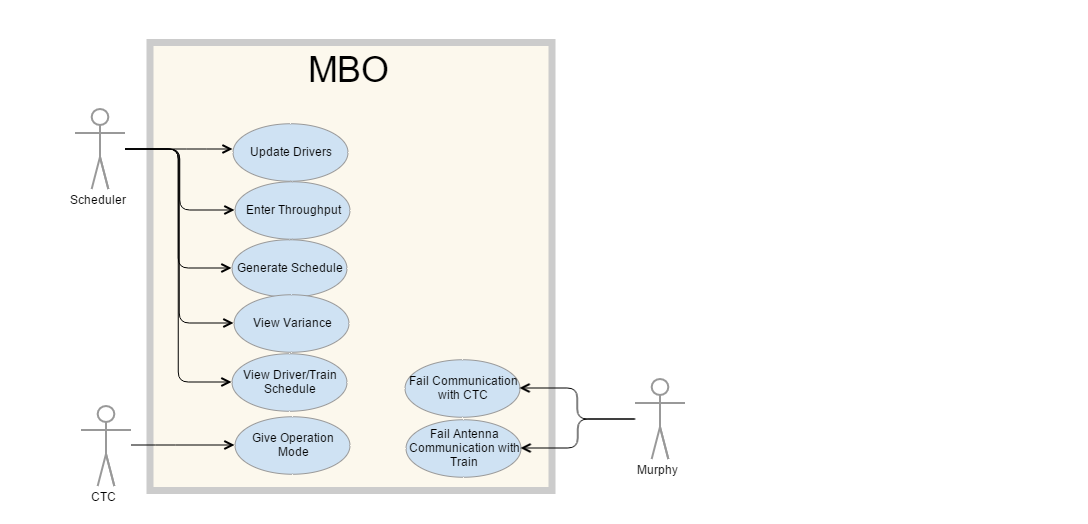
\includegraphics[scale=.5]{mbousecase.png}
	\caption{MBO use case diagram}
\end{figure}
\begin{table}[H]
	\centering
	\caption{Update}
	\begin{tabular}{|l|l|}
		\hline
		Actors & \parbox[t]{10cm}{Scheduler} \\ \hline
		Description & \parbox[t]{10cm}{The Scheduler is able to update the list of drivers. This will change whether or not a driver is able to be scheduled.} \\ \hline
		Data &  \parbox[t]{10cm}{filename} \\ \hline
		Stimulus &  \parbox[t]{10cm}{Click drivers button} \\ \hline
		Response & \parbox[t]{10cm}{Loops through a CSV file to add all the drivers to the list of drivers. When adding a driver, a driver object will be created with the entered properties. This object will then be added to the Driver Schedule where it can be accessed as part of the list.}\\ \hline
		Comments & \parbox[t]{10cm}{There will be a default file so that it can be saved between sessions.}  \\ \hline
	\end{tabular}
\end{table}

\begin{table}[H]
	\centering
	\caption{Enter Throughput}
	\begin{tabular}{|l|l|}
		\hline
		Actors & \parbox[t]{10cm}{Scheduler} \\ \hline
		Description & \parbox[t]{10cm}{The Scheduler enters the number of trains they would like to be on the track at a certain point in time.} \\ \hline
		Data &  \parbox[t]{10cm}{number of trains} \\ \hline
		Stimulus &  \parbox[t]{10cm}{Click submit button} \\ \hline
		Response & \parbox[t]{10cm}{The number of trains is entered by the scheduler. This is used to generate both the train and driver schedules for both MBO and FB modes.}\\ \hline
		Comments & \parbox[t]{10cm}{}  \\ \hline
	\end{tabular}
\end{table}

\begin{table}[H]
	\centering
	\caption{View Train/Driver Schedule}
	\begin{tabular}{|l|l|}
		\hline
		Actors & \parbox[t]{10cm}{Scheduler, CTC} \\ \hline
		Description & \parbox[t]{10cm}{Scheduler can see a list of all  trains, as well as their station arrival times. Scheduler can see a list of all current drivers, as well as their corresponding break times and current train. } \\ \hline
		Data &  \parbox[t]{10cm}{train ID, arrival times, driver name, ID, break times} \\ \hline
		Stimulus &  \parbox[t]{10cm}{Updates triggered by clock} \\ \hline
		Response & \parbox[t]{10cm}{Two tables will be displayed, one for the train schedule, and one for the driver schedule. The train schedule will list IDs as the rows and station names as the columns. Each cell will contain the time that train will arrive at that station. The driver schedule will what train they are on at what times. It will also show whenever they start and stop work and when they are on breaks.}\\ \hline
		Comments & \parbox[t]{10cm}{The table that is displayed will automatically update itself when triggered by the clock.}  \\ \hline
	\end{tabular}
\end{table}

\begin{table}[H]
	\centering
	\caption{View Variance}
	\begin{tabular}{|l|l|}
		\hline
		Actors & \parbox[t]{10cm}{Scheduler} \\ \hline
		Description & \parbox[t]{10cm}{Scheduler can see a list of all  trains, as well as their corresponding speed and current position. The suggested speed and authority will be displayed as well as the variance between the two.} \\ \hline
		Data &  \parbox[t]{10cm}{train ID, speed, suggested/actual position/authority, variance} \\ \hline
		Stimulus &  \parbox[t]{10cm}{Updates triggered by clock} \\ \hline
		Response & \parbox[t]{10cm}{In Fixed Block mode the current block will have to be kept track of based on past block occupancy. In MBO mode the position can be gotten through GPS.}\\ \hline
		Comments & \parbox[t]{10cm}{In Fixed Block mode the position is denoted as the current block. In MBO mode the position is denoted as the current block and the distance into that block.}  \\ \hline
	\end{tabular}
\end{table}

\begin{table}[H]
	\centering
	\caption{Generate Schedules}
	\begin{tabular}{|l|l|}
		\hline
		Actors & \parbox[t]{10cm}{Scheduler} \\ \hline
		Description & \parbox[t]{10cm}{When required a schedule will be generated based on the input data. This will then be displayed for the scheduler/CTC. It is used to dispatch trains and calculate a path for a train.} \\ \hline
		Data &  \parbox[t]{10cm}{number of trains, track data} \\ \hline
		Stimulus &  \parbox[t]{10cm}{On launch, change in number of drivers, clock triggered} \\ \hline
		Response & \parbox[t]{10cm}{A schedule will be generated for trains and drivers. It will have to take into account the mode of operation (MBO or FB), speed limits, track occupancy, drivers’ break times, and other variables.}\\ \hline
		Comments & \parbox[t]{10cm}{Can only happen in automatic mode - schedule will be either fixed block or MBO depending on dispatcher's selection of mode.}  \\ \hline
	\end{tabular}
\end{table}

\begin{table}[H]
	\centering
	\caption{Give Operation Mode}
	\begin{tabular}{|l|l|}
		\hline
		Actors & \parbox[t]{10cm}{CTC} \\ \hline
		Description & \parbox[t]{10cm}{The CTC sends the mode of operation whenever it is changed.} \\ \hline
		Data &  \parbox[t]{10cm}{mode} \\ \hline
		Stimulus &  \parbox[t]{10cm}{CTC changes the mode.} \\ \hline
		Response & \parbox[t]{10cm}{The mode is updated in the MovingBlockOverlay class. Any “shutdown” procedures to switch between modes are performed.}\\ \hline
		Comments & \parbox[t]{10cm}{The default mode will be manual.}  \\ \hline
	\end{tabular}
\end{table}

\begin{table}[H]
	\centering
	\caption{Fail Communication with CTC}
	\begin{tabular}{|l|l|}
		\hline
		Actors & \parbox[t]{10cm}{Murphy} \\ \hline
		Description & \parbox[t]{10cm}{Murphy breaks communication between CTC and MBO.} \\ \hline
		Data &  \parbox[t]{10cm}{communication failure} \\ \hline
		Stimulus &  \parbox[t]{10cm}{CTC clicks Fail Communication with MBO button.} \\ \hline
		Response & \parbox[t]{10cm}{Since scheduling will be unavailable without communication with the MBO, the CTC will be forced into manual mode and let the dispatcher know with a message.}\\ \hline
		Comments & \parbox[t]{10cm}{}  \\ \hline
	\end{tabular}
\end{table}

\begin{table}[H]
	\centering
	\caption{Fail Communication with Train}
	\begin{tabular}{|l|l|}
		\hline
		Actors & \parbox[t]{10cm}{Murphy} \\ \hline
		Description & \parbox[t]{10cm}{Murphy breaks communication between Train and wayside.} \\ \hline
		Data &  \parbox[t]{10cm}{communication failure} \\ \hline
		Stimulus &  \parbox[t]{10cm}{Click Fail Communication with Train button.} \\ \hline
		Response & \parbox[t]{10cm}{The MBO can no longer receive the GPS position of individual trains and is therefore unable to safely operate in MBO mode. So a transition must be made to either Fixed Block mode or to manual mode.}\\ \hline
		Comments & \parbox[t]{10cm}{}  \\ \hline
	\end{tabular}
\end{table}

\subsection{Centralized Train Control}
In this subsection, the use cases of the Centralized Train Control (CTC) are provided.
\begin{figure}[H]
	\centering
	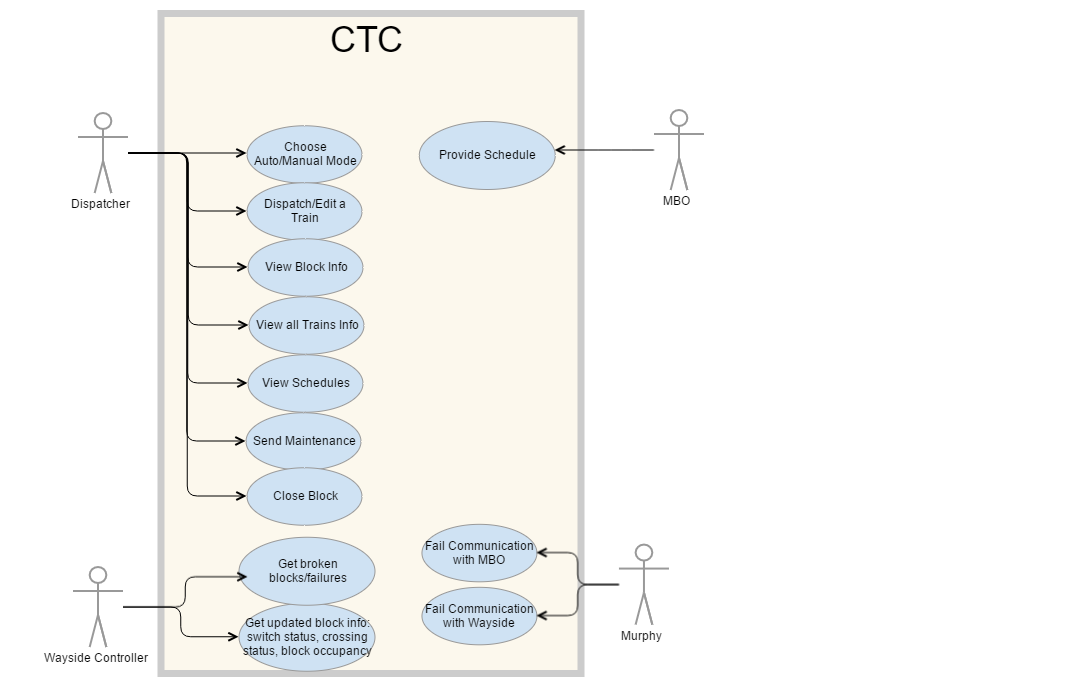
\includegraphics[scale=.5]{ctcusecase.png}
	\caption{Centralized Train Control use case}
\end{figure}

\begin{table}[H]
	\centering
	\caption{Choose Auto/Manual Mode}
	\begin{tabular}{|l|l|}
		\hline
		Actors & \parbox[t]{10cm}{Dispatcher} \\ \hline
		Description & \parbox[t]{10cm}{Dispatcher can choose between automatic and manual mode. Automatic can then be either MBO or fixed block mode. Automatic uses a schedule while manual allows the dispatcher to send out trains.} \\ \hline
		Data &  \parbox[t]{10cm}{Mode Selection: manual vs automatic, and MBO vs fixed block (only if auto chosen)} \\ \hline
		Stimulus &  \parbox[t]{10cm}{Radio button selections} \\ \hline
		Response & \parbox[t]{10cm}{Automatic passes a schedule along to the other applicable modules. Schedule can also be viewed by dispatcher as well as disabling the Trains Panel. Manual enables the manual dispatching of trains via the Trains Panel but disables viewing a schedule.}\\ \hline
		Comments & \parbox[t]{10cm}{Can be triggered at any time - no previous requirements needed. }  \\ \hline
	\end{tabular}
\end{table}

\begin{table}[H]
	\centering
	\caption{Dispatch/Edit a Train}
	\begin{tabular}{|l|l|}
		\hline
		Actors & \parbox[t]{10cm}{Dispatcher} \\ \hline
		Description & \parbox[t]{10cm}{When in manual mode, the dispatcher is responsible for dispatching new trains from the yard or editing a train's speed and authority as it goes around the track.} \\ \hline
		Data &  \parbox[t]{10cm}{Speed, authority, train ID, current block of train} \\ \hline
		Stimulus &  \parbox[t]{10cm}{Click dispatch or edit a train buttons in Train Panel.} \\ \hline
		Response & \parbox[t]{10cm}{Speed and authority are given to the wayside. If it is a new train, the ID will be -1 and will be updated by the train model. If it is a preexisting train, the ID will be a passed integer value. The ID is passed to the track model.}\\ \hline
		Comments & \parbox[t]{10cm}{Can only happen in manual mode. It is completely disabled in automatic mode.}  \\ \hline
	\end{tabular}
\end{table}

\begin{table}[H]
	\centering
	\caption{View Block Info}
	\begin{tabular}{|l|l|}
		\hline
		Actors & \parbox[t]{10cm}{Dispatcher} \\ \hline
		Description & \parbox[t]{10cm}{Dispatcher can see information relating to a chosen block on the track.} \\ \hline
		Data &  \parbox[t]{10cm}{Block} \\ \hline
		Stimulus &  \parbox[t]{10cm}{Choose line, segment, block from dropdown menu.} \\ \hline
		Response & \parbox[t]{10cm}{After choosing from dropdowns, info relating to this block of the track will be displayed. This info includes: if there is a station/crossing/switch, station name/switch number/switch state/crossing state if applicable, block occupancy and speed limit.}\\ \hline
		Comments & \parbox[t]{10cm}{Will auto update in real time if this info changes while the block remains selected on the screen.}  \\ \hline
	\end{tabular}
\end{table}

\begin{table}[H]
	\centering
	\caption{View All Trains}
	\begin{tabular}{|l|l|}
		\hline
		Actors & \parbox[t]{10cm}{Dispatcher} \\ \hline
		Description & \parbox[t]{10cm}{Dispatcher can see a list of all current trains, as well as their corresponding speed and current position.} \\ \hline
		Data &  \parbox[t]{10cm}{train ID, speed, position/authority} \\ \hline
		Stimulus &  \parbox[t]{10cm}{Click View Trains button.} \\ \hline
		Response & \parbox[t]{10cm}{After clicking this button, a list of trains will appear by line, followed by their IDs, speed, and current position/authority (depending on the mode).}\\ \hline
		Comments & \parbox[t]{10cm}{What info is displayed will depend on the current mode selected.}  \\ \hline
	\end{tabular}
\end{table}

\begin{table}[H]
	\centering
	\caption{View Schedules}
	\begin{tabular}{|l|l|}
		\hline
		Actors & \parbox[t]{10cm}{Dispatcher} \\ \hline
		Description & \parbox[t]{10cm}{Dispatcher can see the schedule for both lines and all trains.} \\ \hline
		Data &  \parbox[t]{10cm}{schedule from MBO} \\ \hline
		Stimulus &  \parbox[t]{10cm}{Click View Schedule button.} \\ \hline
		Response & \parbox[t]{10cm}{After clicking this button, the train schedule per line will appear as sent from the MBO.}\\ \hline
		Comments & \parbox[t]{10cm}{Can only happen in automatic mode - schedule will be either fixed block or MBO depending on dispatcher's selection of mode.}  \\ \hline
	\end{tabular}
\end{table}

\begin{table}[H]
	\centering
	\caption{Send Maintenance}
	\begin{tabular}{|l|l|}
		\hline
		Actors & \parbox[t]{10cm}{Dispatcher} \\ \hline
		Description & \parbox[t]{10cm}{Dispatcher sends maintenance when a block is broken but only after the broken block is closed.} \\ \hline
		Data &  \parbox[t]{10cm}{block, closed status} \\ \hline
		Stimulus &  \parbox[t]{10cm}{Click Send Maintenance button.} \\ \hline
		Response & \parbox[t]{10cm}{After clicking this button, the block will be fixed by maintenance personnel and the block will be automatically re-opened.}\\ \hline
		Comments & \parbox[t]{10cm}{Can only happen after a block is empty and successfully closed.}  \\ \hline
	\end{tabular}
\end{table}

\begin{table}[H]
	\centering
	\caption{Close Block}
	\begin{tabular}{|l|l|}
		\hline
		Actors & \parbox[t]{10cm}{Dispatcher} \\ \hline
		Description & \parbox[t]{10cm}{Dispatcher closes a block when informed of a failure via the wayside.} \\ \hline
		Data &  \parbox[t]{10cm}{block, failure status} \\ \hline
		Stimulus &  \parbox[t]{10cm}{Click Close Block button.} \\ \hline
		Response & \parbox[t]{10cm}{After clicking this button, the block will be closed and emptied of trains. Any trains around it will be rereouted or stopped as necessary.}\\ \hline
		Comments & \parbox[t]{10cm}{Can only happen when block failure status changes from good to broken.}  \\ \hline
	\end{tabular}
\end{table}

\begin{table}[H]
	\centering
	\caption{Fail Communication with MBO}
	\begin{tabular}{|l|l|}
		\hline
		Actors & \parbox[t]{10cm}{Murphy} \\ \hline
		Description & \parbox[t]{10cm}{Murphy breaks communication between CTC and MBO.} \\ \hline
		Data &  \parbox[t]{10cm}{communication failure} \\ \hline
		Stimulus &  \parbox[t]{10cm}{Click Fail Communication with MBO button.} \\ \hline
		Response & \parbox[t]{10cm}{Since scheduling will be unavailable without communication with the MBO, the CTC will be forced into manual mode and let the dispatcher know with a message.}\\ \hline
		Comments & \parbox[t]{10cm}{ }  \\ \hline
	\end{tabular}
\end{table}

\begin{table}[H]
	\centering
	\caption{Fail Communication with Wayside}
	\begin{tabular}{|l|l|}
		\hline
		Actors & \parbox[t]{10cm}{Murphy} \\ \hline
		Description & \parbox[t]{10cm}{Murphy breaks communication between CTC and wayside.} \\ \hline
		Data &  \parbox[t]{10cm}{communication failure} \\ \hline
		Stimulus &  \parbox[t]{10cm}{Click Fail Communication with Wayside button.} \\ \hline
		Response & \parbox[t]{10cm}{Since the wayside is vital, all trains will be alerted to stop as this is the safest thing to do. They will be instructed to start up again only when communications resume.}\\ \hline
		Comments & \parbox[t]{10cm}{ }  \\ \hline
	\end{tabular}
\end{table}

\begin{table}[H]
	\centering
	\caption{Get Schedule}
	\begin{tabular}{|l|l|}
		\hline
		Actors & \parbox[t]{10cm}{MBO} \\ \hline
		Description & \parbox[t]{10cm}{MBO updates schedule and give it to the CTC whenever there is an update to the file.} \\ \hline
		Data &  \parbox[t]{10cm}{train schedule} \\ \hline
		Stimulus &  \parbox[t]{10cm}{Update as schedule changes.} \\ \hline
		Response & \parbox[t]{10cm}{The schedule will be updated whenever the MBO makes any changes and those changes will be reflected should the dispatcher choose to view the schedule in the popup.}\\ \hline
		Comments & \parbox[t]{10cm}{ }  \\ \hline
	\end{tabular}
\end{table}

\begin{table}[H]
	\centering
	\caption{Get Broken Blocks/Failures}
	\begin{tabular}{|l|l|}
		\hline
		Actors & \parbox[t]{10cm}{Wayside} \\ \hline
		Description & \parbox[t]{10cm}{Wayside informs CTC of any broken blocks or failures.} \\ \hline
		Data &  \parbox[t]{10cm}{block} \\ \hline
		Stimulus &  \parbox[t]{10cm}{Updates constantly as wayside receives info from track.} \\ \hline
		Response & \parbox[t]{10cm}{The schedule will be updated whenever the MBO makes any changes and those changes will be reflected should the dispatcher choose to view the schedule in the popup.}\\ \hline
		Comments & \parbox[t]{10cm}{ }  \\ \hline
	\end{tabular}
\end{table}

\begin{table}[H]
	\centering
	\caption{Get Updated Block Info}
	\begin{tabular}{|l|l|}
		\hline
		Actors & \parbox[t]{10cm}{Wayside} \\ \hline
		Description & \parbox[t]{10cm}{Wayside informs CTC of updated info in requested block.} \\ \hline
		Data &  \parbox[t]{10cm}{switch status, crossing status, block occupancy} \\ \hline
		Stimulus &  \parbox[t]{10cm}{Updates with the clock tick as the wayside gets updates from the track, info then goes to CTC.} \\ \hline
		Response & \parbox[t]{10cm}{These changes will be reflected on the track panel of the GUI so that the dispatcher can see updated info constantly and react accordingly.}\\ \hline
		Comments & \parbox[t]{10cm}{ }  \\ \hline
	\end{tabular}
\end{table}

\section{Class Diagrams}
In this section, the class diagrams for each subsystem are provided.
\subsection{Track Model}
\begin{figure}[H]
	\centering
	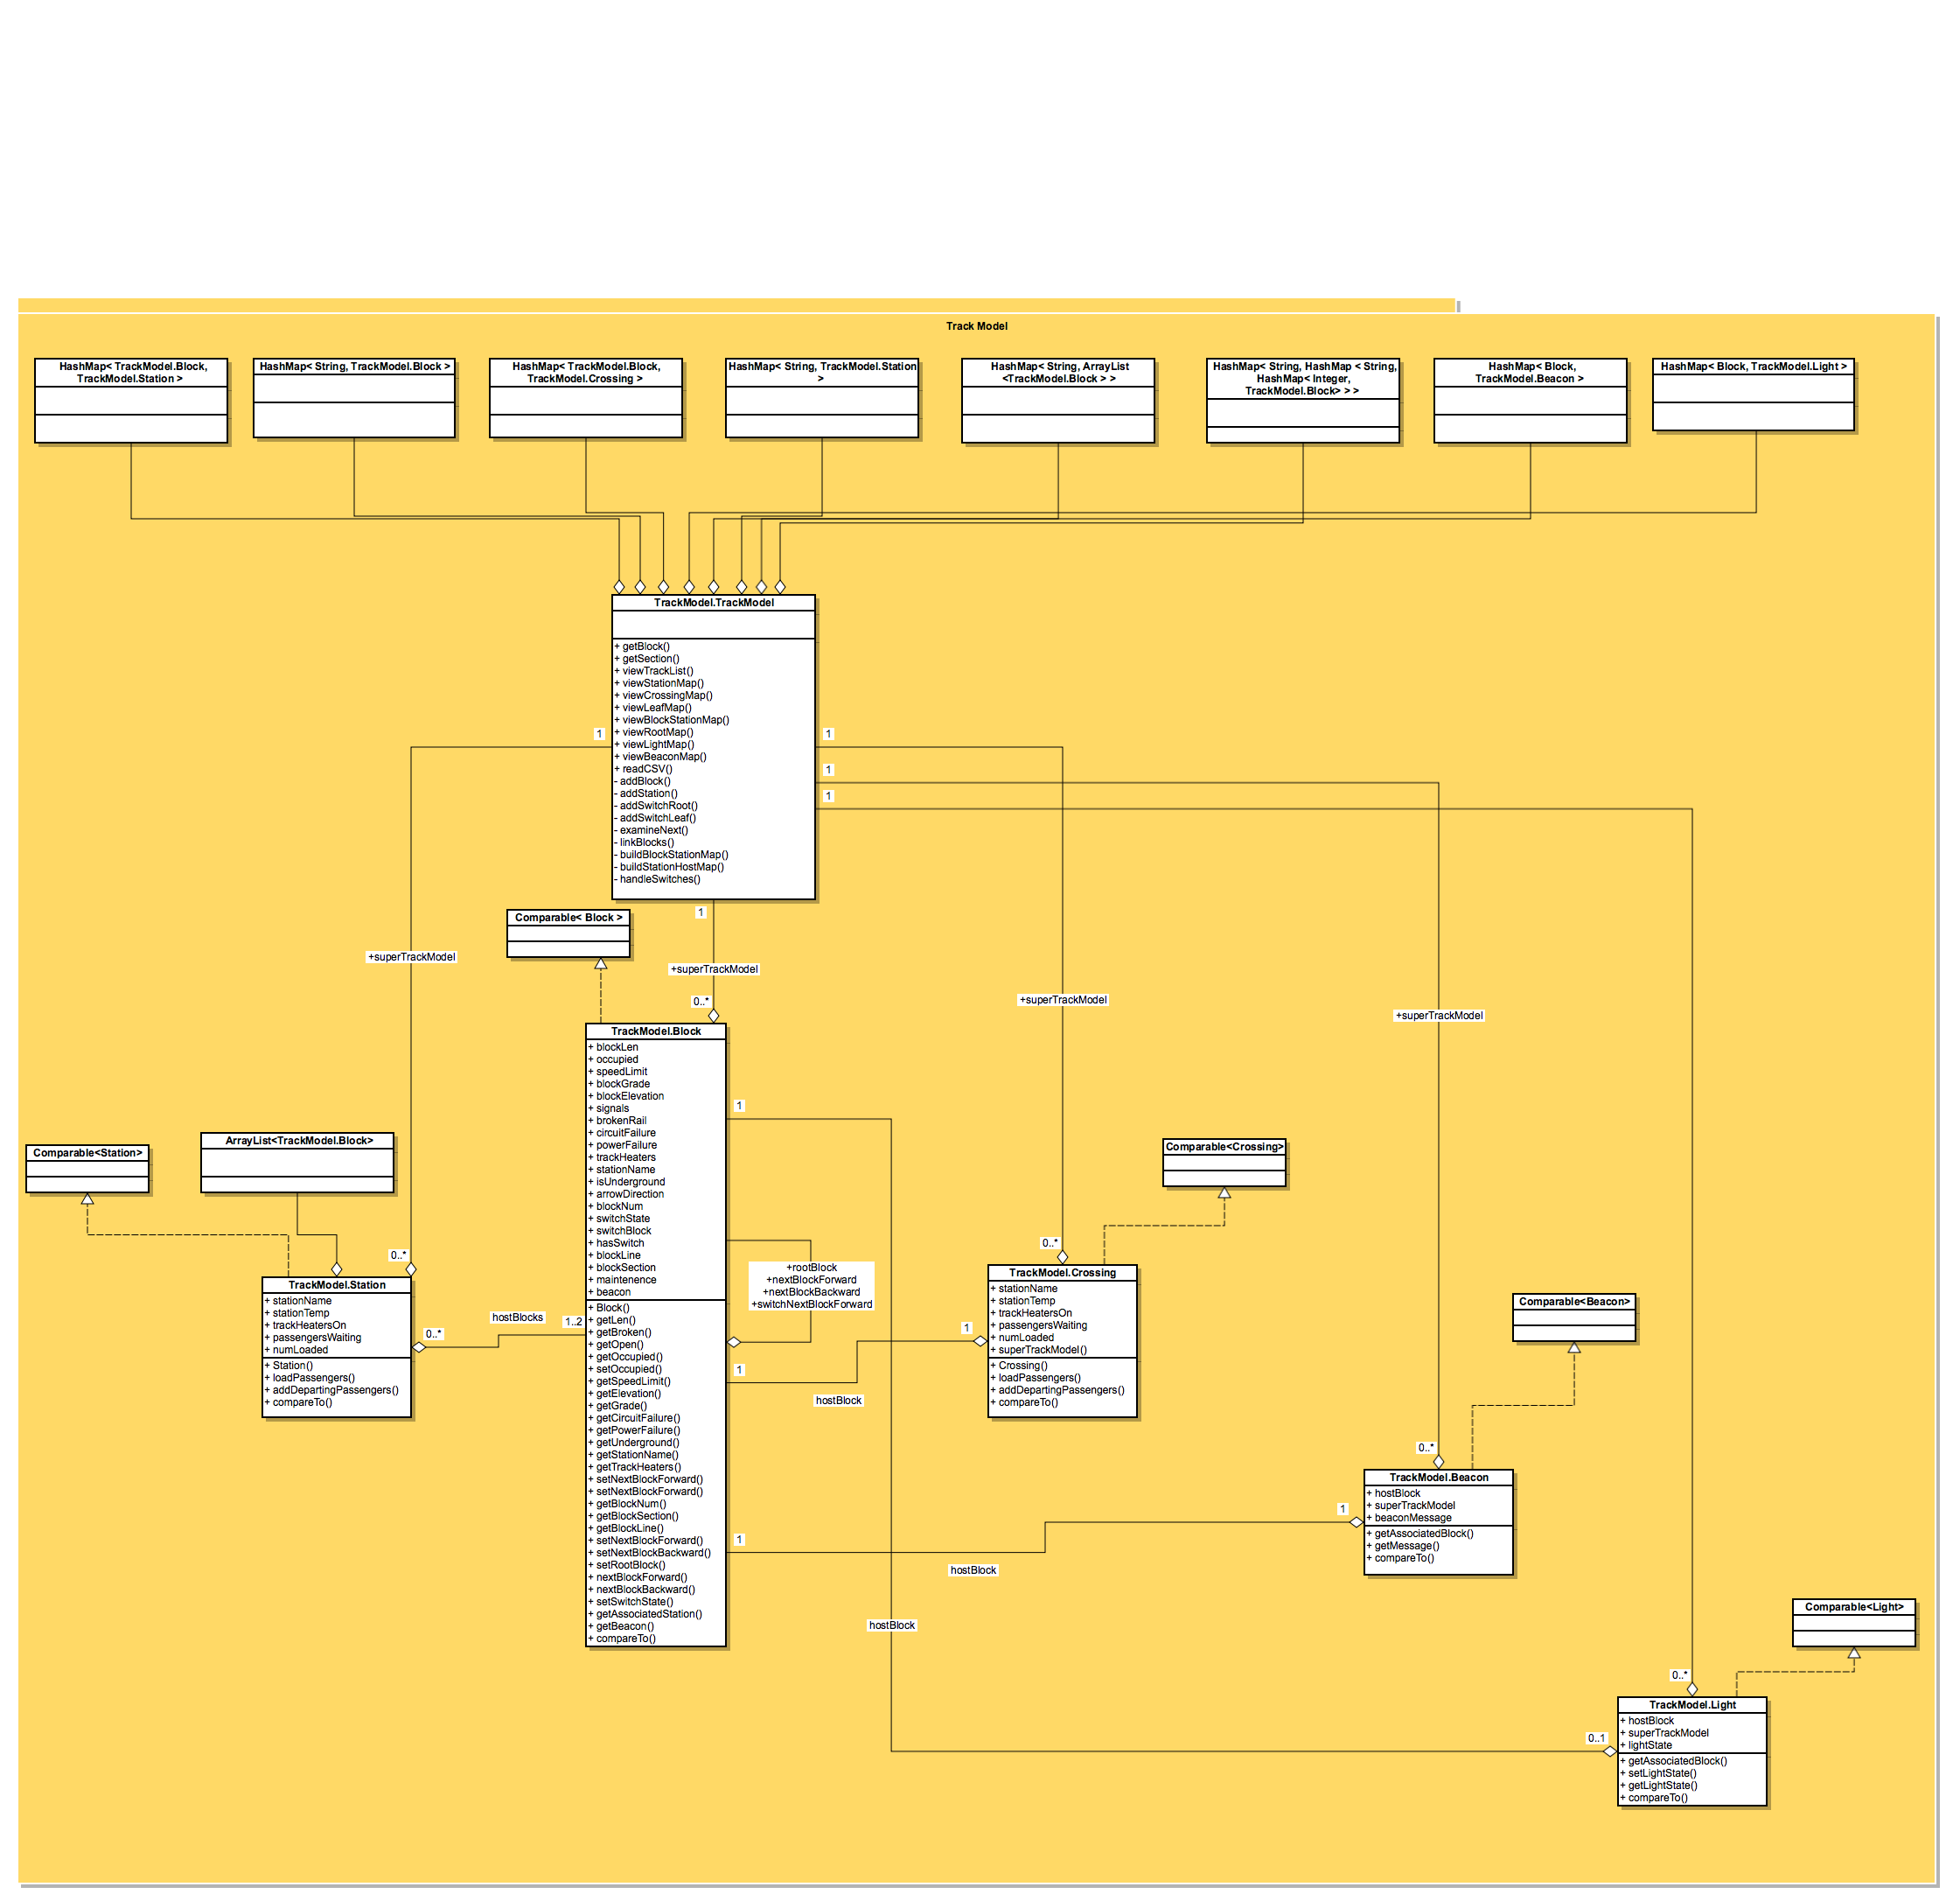
\includegraphics[scale=.2]{trackmodel.png}
	\caption{Track Model Class diagram}
\end{figure}

The track model package consists of a block object to be utilized by all classes, 
\subsection{Track Controller}
	\begin{figure}[H]
		\centering
		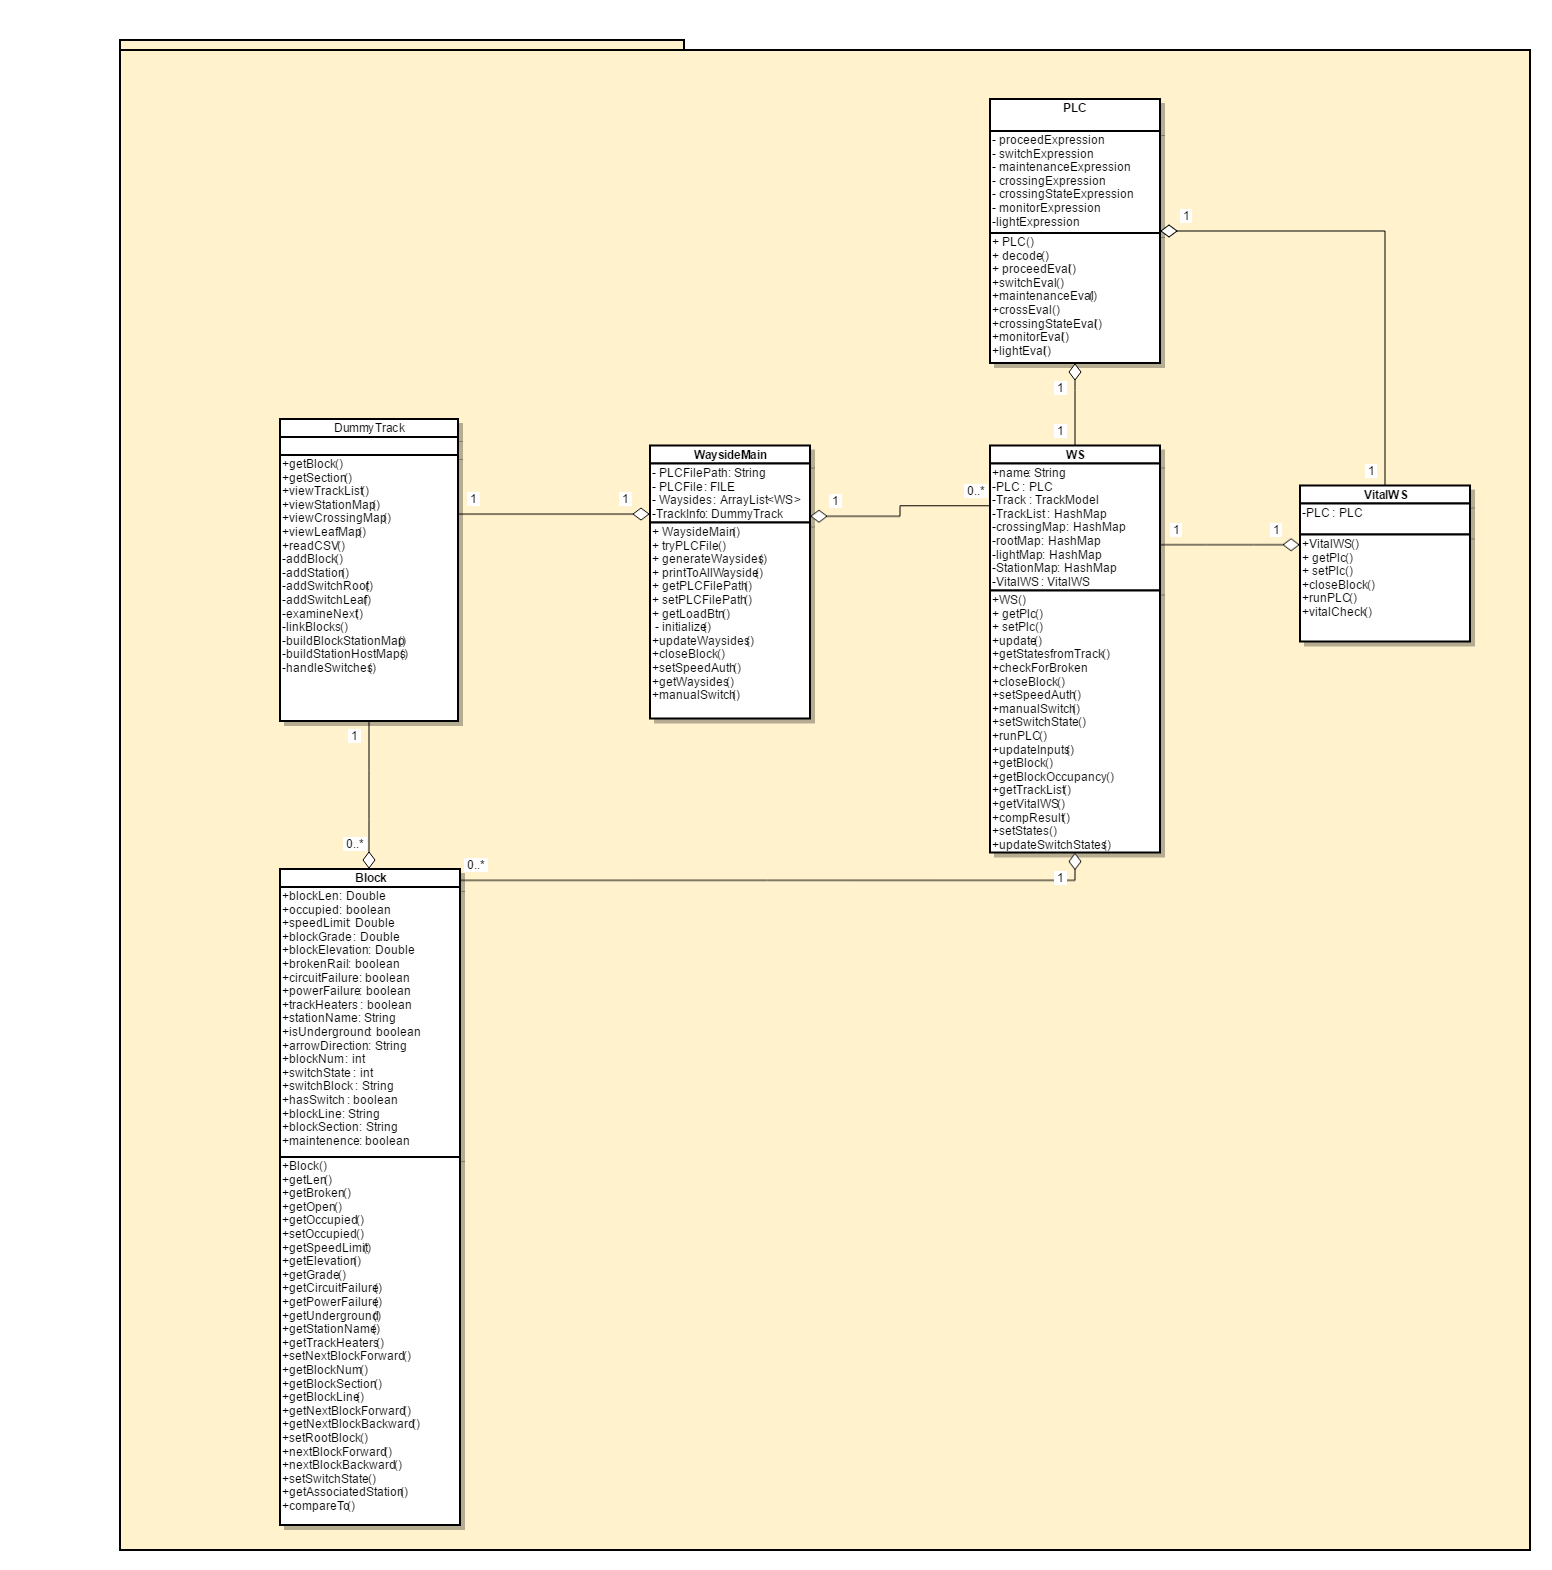
\includegraphics[scale=.25]{trackcontroller.png}
		\caption{Track Controller Class diagram}
	\end{figure}
\subsection{Train Model}
\begin{figure}[H]
	\centering
	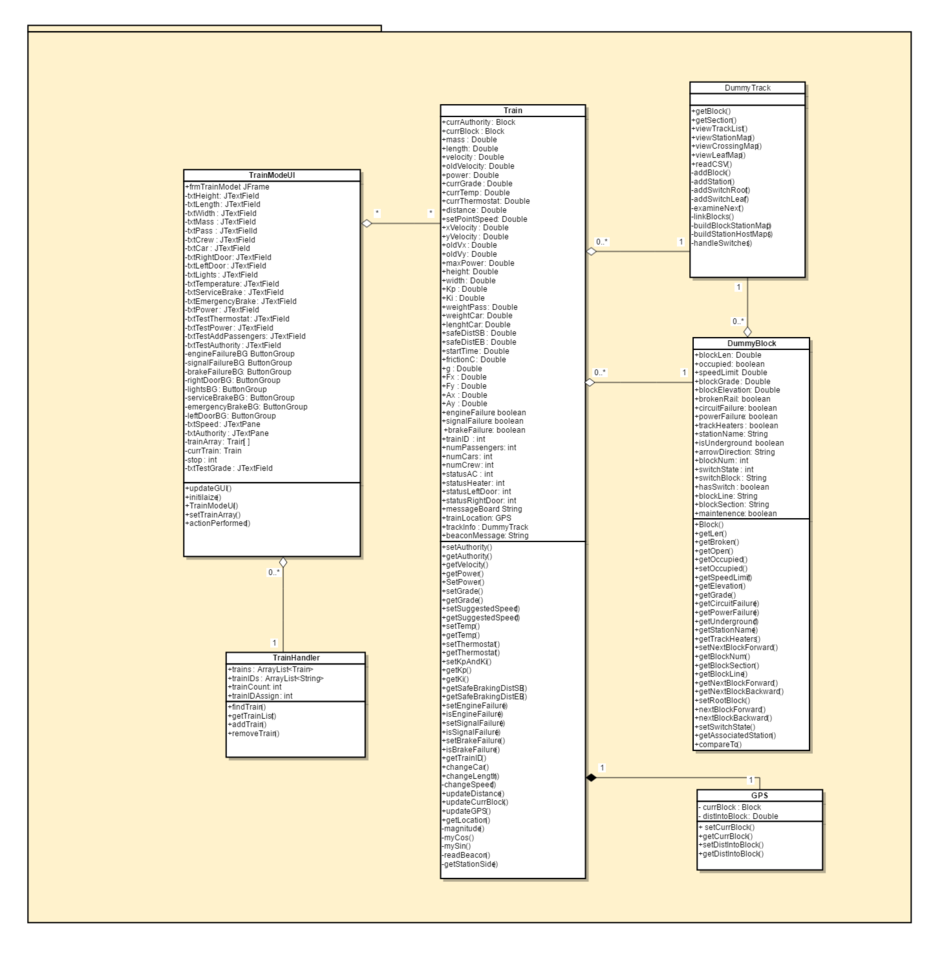
\includegraphics[width=\textwidth]{trainmodelclassdiagram.png}
	\caption{Train Model Class diagram}
\end{figure}

The train model package consists of a train object, a train Handler, a UI class, a GPS object, and a dummyTrack and dummyBlock class. The train class will handle all train properties including utilities, failure statuses, and physics calculations. This will contain ample setters and getters for the train controller to access in order to modify states on board the train as well as change various values. The train handler will contain all trains in the system and will be used to communicate with other modules in order to assure the proper communication paths are followed. The UI class will update a GUI containing all relevant data for the current train being monitored. The GPS class will contain the current location of the train in terms of current block and distance into block and will primarily be used by the MBO in order to calculate exact train positioning. THe DummyTrack and DummyBlock are both classes that will be accessed by the train at startup. They will contain newly intialized copies of the track model with values based on the excel sheet. This will be used in order to compute current block as the train moves through the system to determine the change in grade and other various properties.

\subsection{Train Controller}
\begin{figure}[H]
	\centering
	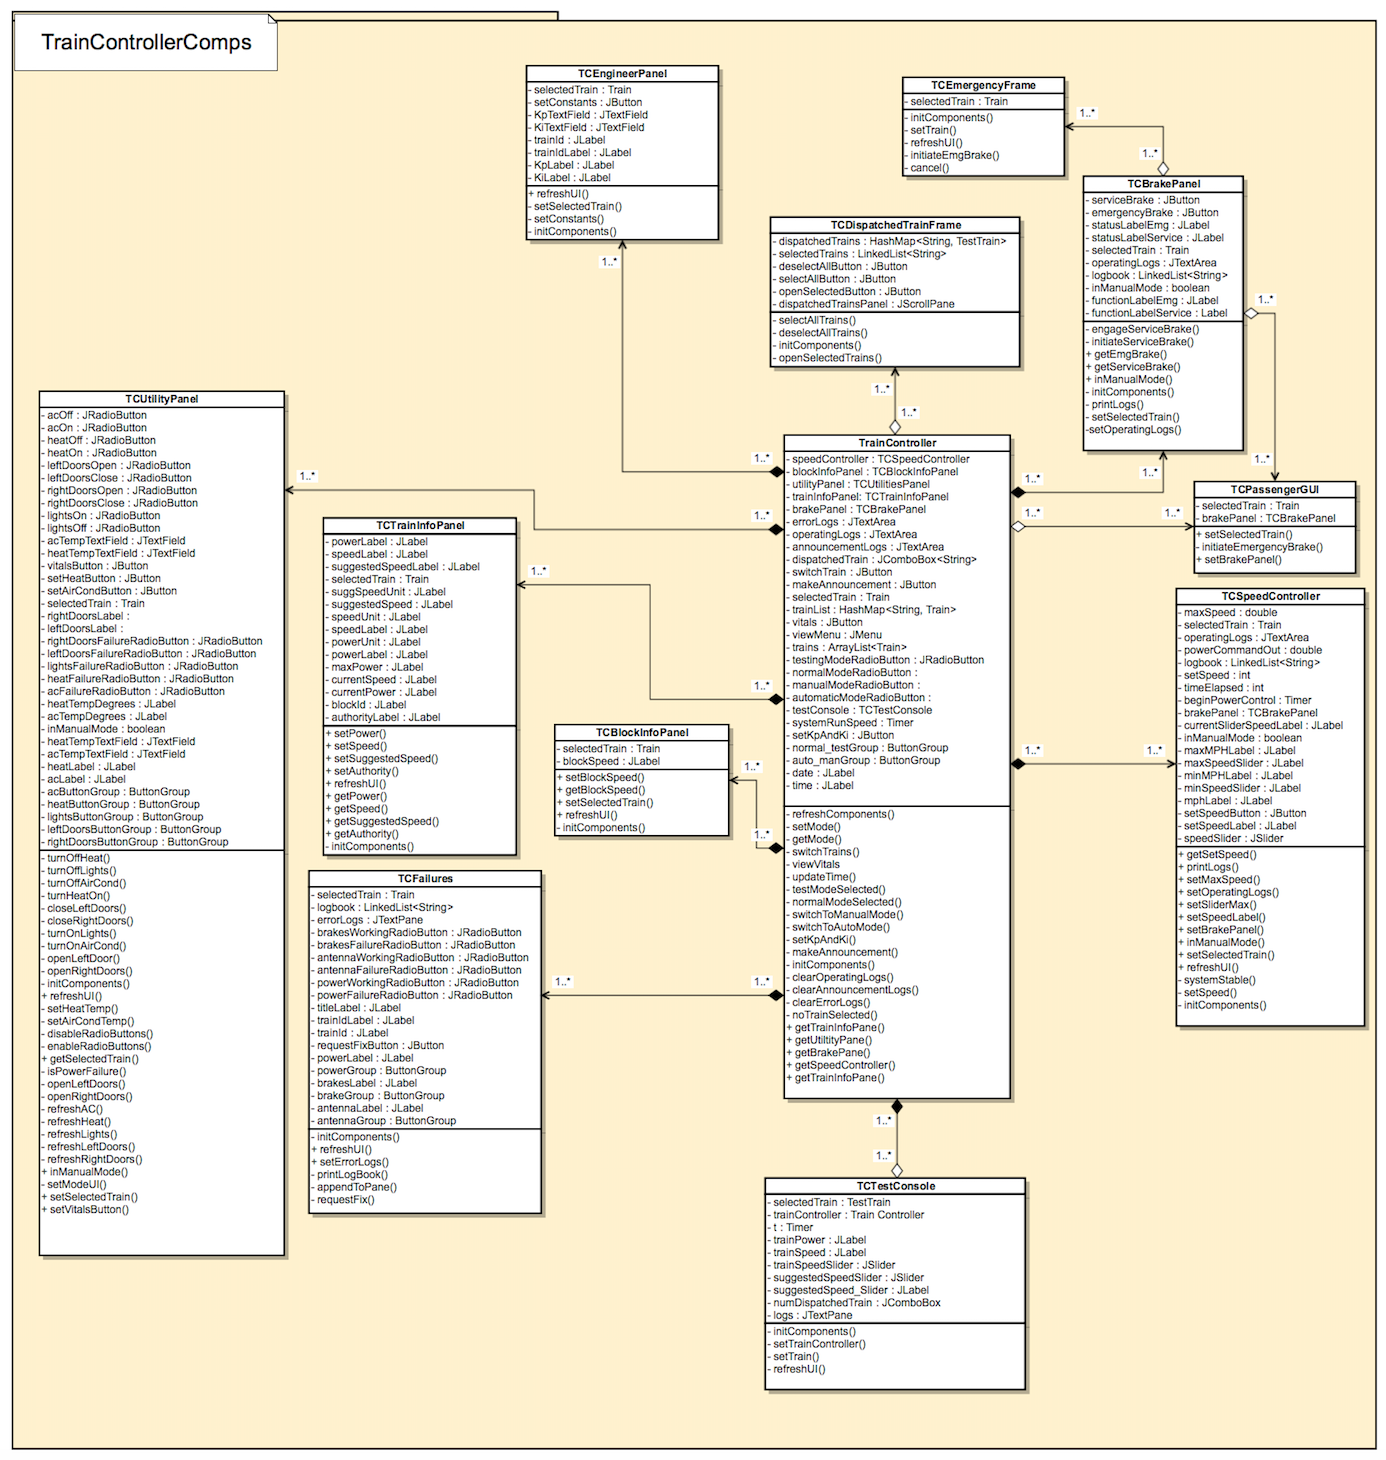
\includegraphics[width=\textwidth]{tc_classdiagram.png}
	\caption{Train Controller Class Diagram}
\end{figure}
\subsection{Moving Block Overlay}
\begin{figure}[H]
	\centering
	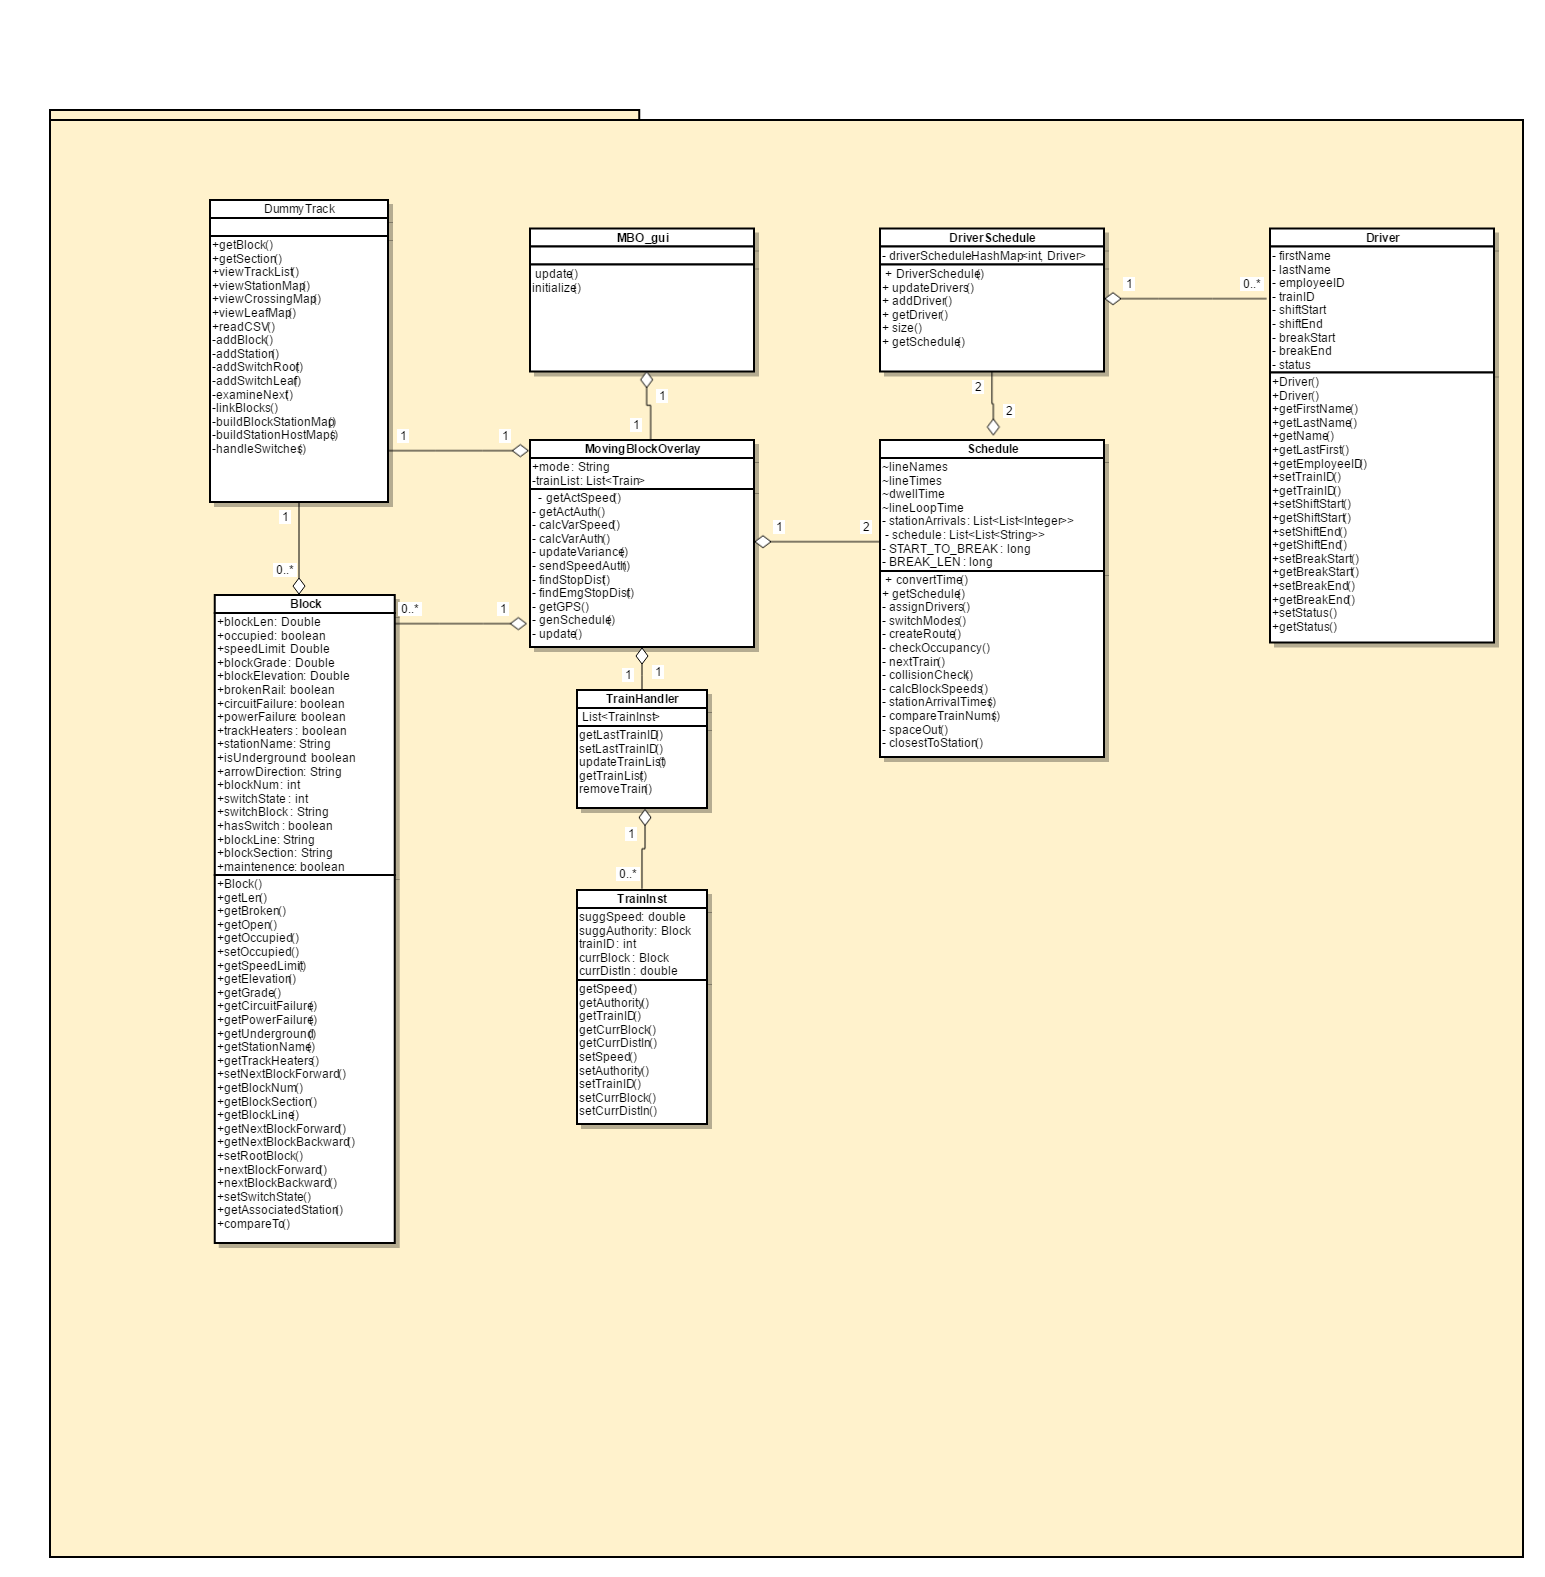
\includegraphics[width=\textwidth]{mbo.png}
	\caption{MBO Class Diagram}
\end{figure}
\subsection{Centralized Train Controller}
\begin{figure}[H]
	\centering
	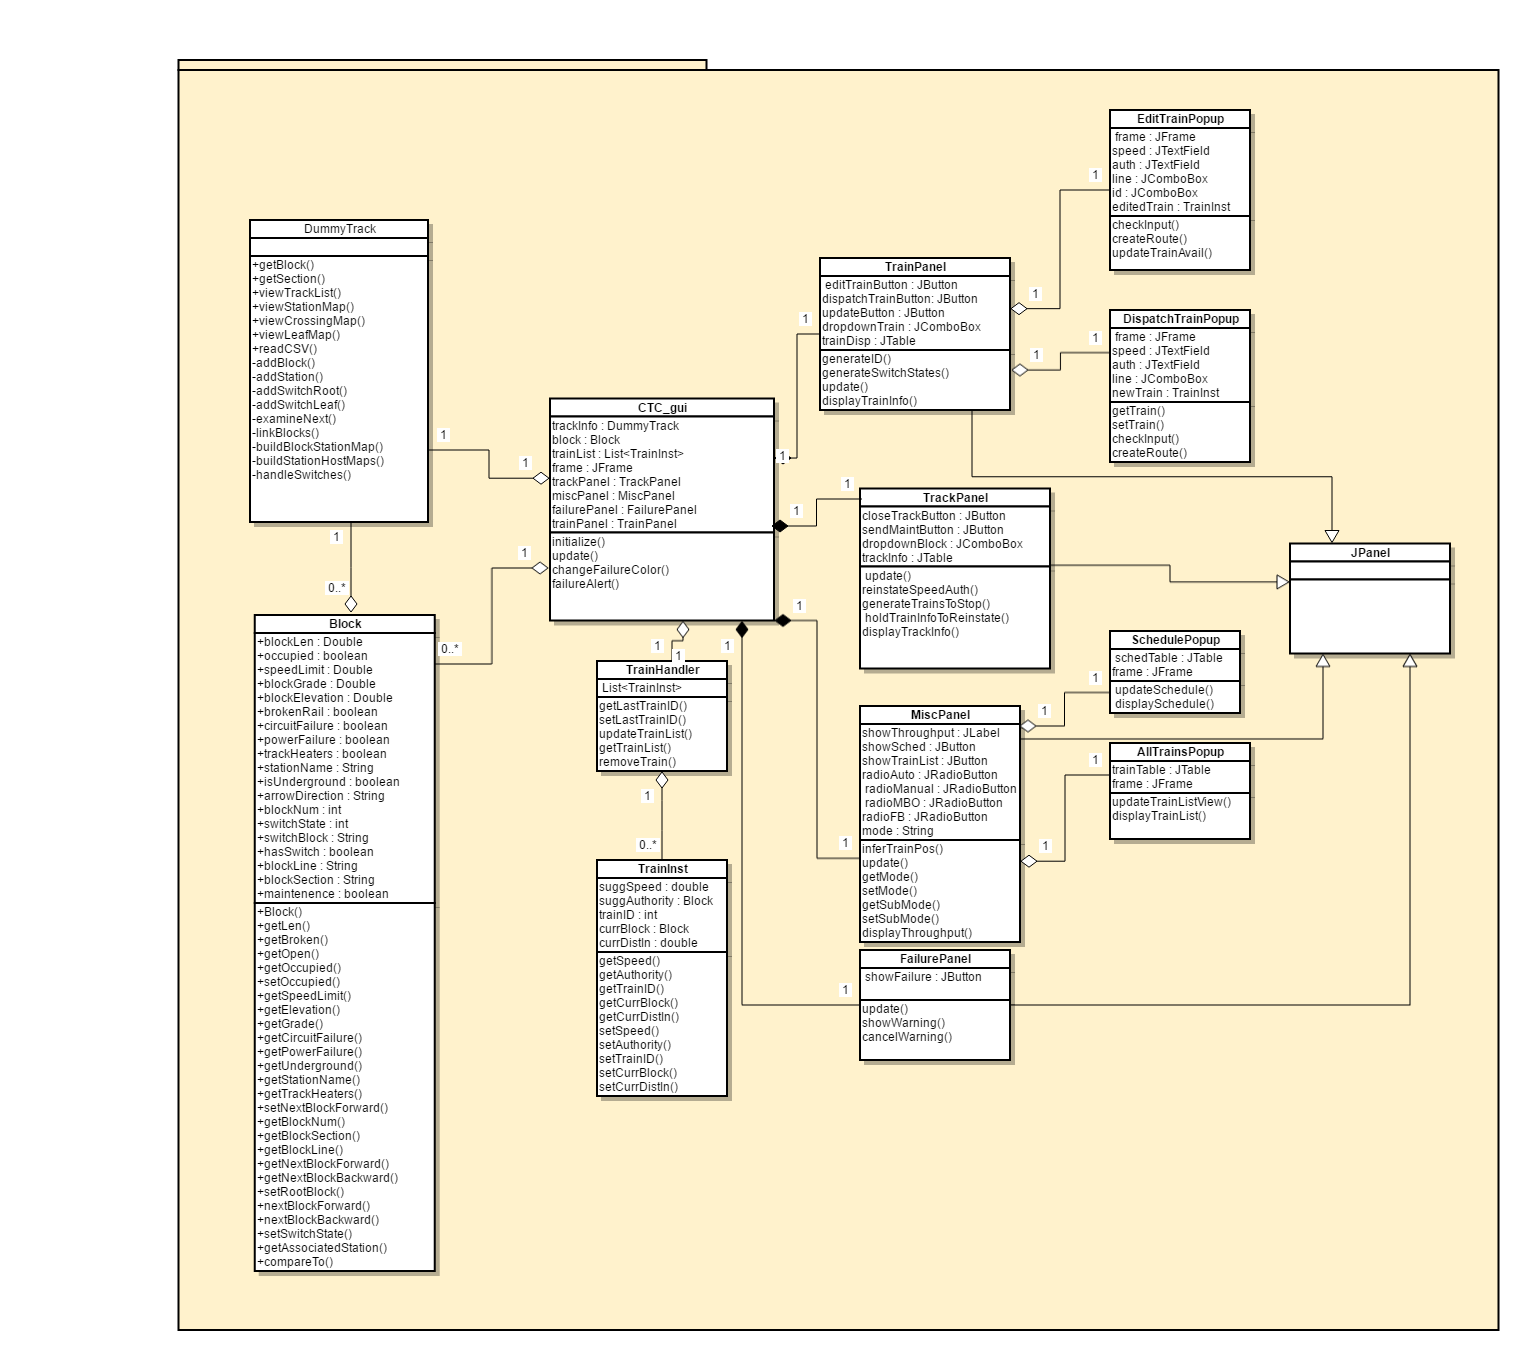
\includegraphics[scale=.2]{ctc.png}
	\caption{CTC Class diagram}
\end{figure}


\section{Sequence Diagrams}
In this section, we detail the sequence diagrams each subsystem.
\subsection{Track Model}
\begin{figure}[H]
	\centering
	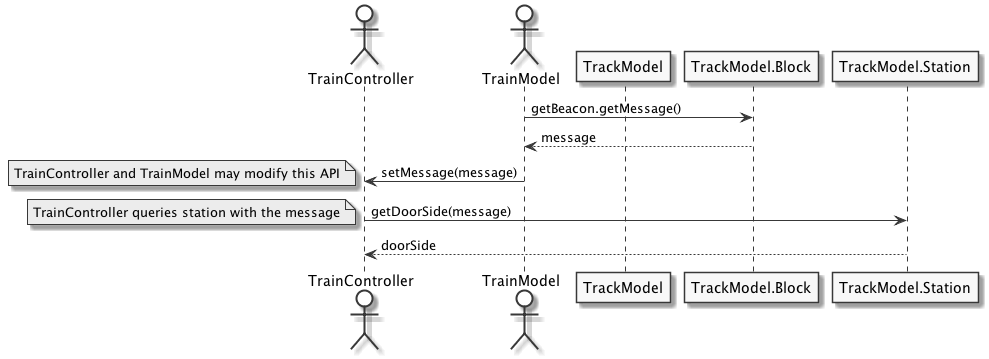
\includegraphics[width=\textwidth]{getStationDirection.png}
	\caption{Getting station direction}
\end{figure}
\begin{table}[H]
	\centering
	\caption{Getting the Door Side to Open on a Train}
	\begin{tabular}{|l|l|}
		\hline
		Actors & \parbox[t]{10cm}{TrainModel, TrainController} \\ \hline
		Description & \parbox[t]{10cm}{The train model gets a message, gives it to the train controller, which calls the station with that beacon direction to get a door side} \\ \hline
		Data &  \parbox[t]{10cm}{The beacon message} \\ \hline
		Stimulus &  \parbox[t]{10cm}{A train reaching a block with a beacon} \\ \hline
		Response & \parbox[t]{10cm}{A message then a door side}\\ \hline
		Comments & \parbox[t]{10cm}{This is a composite action which may not be accurate for actions between the TrainController and TrainModel. While they are assumed to communicate for these purposes, the exact API may not be reflected in this diagram. User should consult pertinent diagrams.}  \\ \hline
	\end{tabular}
\end{table}


\begin{figure}[H]
	\centering
	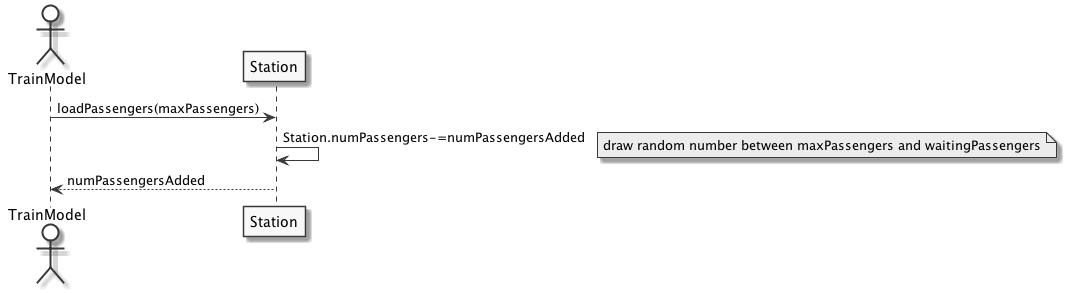
\includegraphics[width=\textwidth]{addPassengers.png}
	\caption{Add Passengers Sequence Diagram}
\end{figure}
\begin{table}[H]
	\centering
	\caption{Adding passengers}
	\begin{tabular}{|l|l|}
		\hline
		Actors & \parbox[t]{10cm}{TrainModel} \\ \hline
		Description & \parbox[t]{10cm}{The train model calls the station to load passengers to a train} \\ \hline
		Data &  \parbox[t]{10cm}{maximum number of passengers to add to a train} \\ \hline
		Stimulus &  \parbox[t]{10cm}{A train model calling the station} \\ \hline
		Response & \parbox[t]{10cm}{A number of people to add to a given train model}\\ \hline
		Comments & \parbox[t]{10cm}{The passengers added to the trainmodel are removed from the passengers waiting at the station}  \\ \hline
	\end{tabular}
\end{table}

\begin{figure}[H]
	\centering
	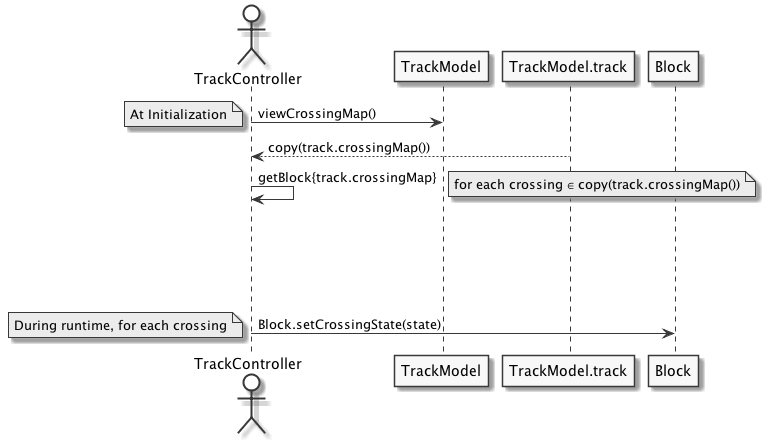
\includegraphics[scale=.5]{crossing.png}
	\caption{Toggle Crossing State Sequence Diagram}
\end{figure}

\begin{table}[H]
	\centering
	\caption{Toggle crossing state description}
	\begin{tabular}{|l|l|}
		\hline
		Actors & \parbox[t]{10cm}{TrackController} \\ \hline
		Description & \parbox[t]{10cm}{The track controller first indexes all the switches on a given track at initialization. The track controller then calls the toggleCrossing function on each block } \\ \hline
		Data &  \parbox[t]{10cm}{A boolean state represented as an Integer} \\ \hline
		Stimulus &  \parbox[t]{10cm}{A track controller call} \\ \hline
		Response & \parbox[t]{10cm}{Setting the boolean state of the crossing based on the TrackController}\\ \hline
		Comments & \parbox[t]{10cm}{Blocks without a crossing have a null in lieu of an integer}  \\ \hline
	\end{tabular}
\end{table}

\begin{figure}[H]
	\centering
	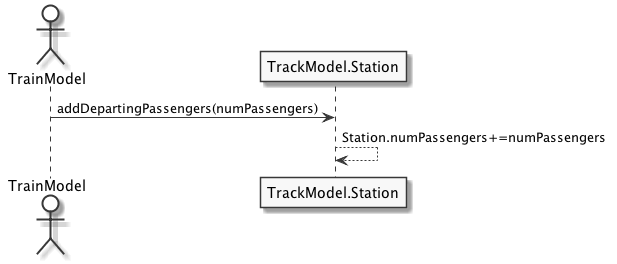
\includegraphics[scale=.5]{departPassengers.png}
	\caption{Departing Passengers to Station Use Case Diagram}
\end{figure}
\begin{table}[H]
	\centering
	\caption{Depart Passengers to a Station}
	\begin{tabular}{|l|l|}
		\hline
		Actors & \parbox[t]{10cm}{TrainModel} \\ \hline
		Description & \parbox[t]{10cm}{The train model calls the station to depart passengers from a train} \\ \hline
		Data &  \parbox[t]{10cm}{Number of passengers to depart} \\ \hline
		Stimulus &  \parbox[t]{10cm}{A train model calling the station} \\ \hline
		Response & \parbox[t]{10cm}{The number of people departing the train are added to the people waiting at a station}\\ \hline
		Comments & \parbox[t]{10cm}{The passengers in the system are assumed to be finite and a closed model in this system}  \\ \hline
	\end{tabular}
\end{table}

\begin{figure}[H]
	\centering
	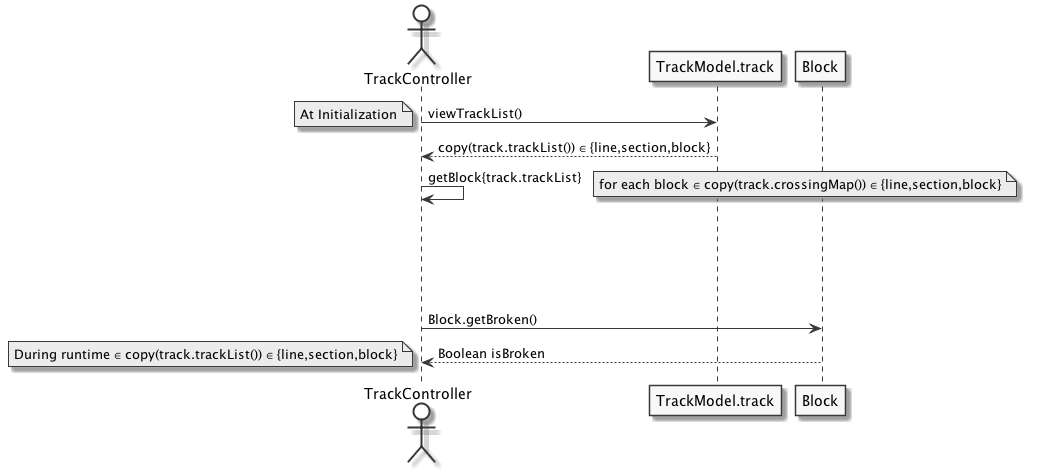
\includegraphics[width=\textwidth]{detectBroken.png}
	\caption{Detect Broken Rail Sequence Diagram}
\end{figure}

\begin{table}[H]
	\centering
	\caption{Detect broken rail}
	\begin{tabular}{|l|l|}
		\hline
		Actors & \parbox[t]{10cm}{TrackController} \\ \hline
		Description & \parbox[t]{10cm}{The track controller iterates over the track to identify any broken rails} \\ \hline
		Data &  \parbox[t]{10cm}{None} \\ \hline
		Stimulus &  \parbox[t]{10cm}{None} \\ \hline
		Response & \parbox[t]{10cm}{None}\\ \hline
		Comments & \parbox[t]{10cm}{The TrackController is responsible for identifying broken rails}  \\ \hline
	\end{tabular}
\end{table}

\begin{figure}[H]
	\centering
	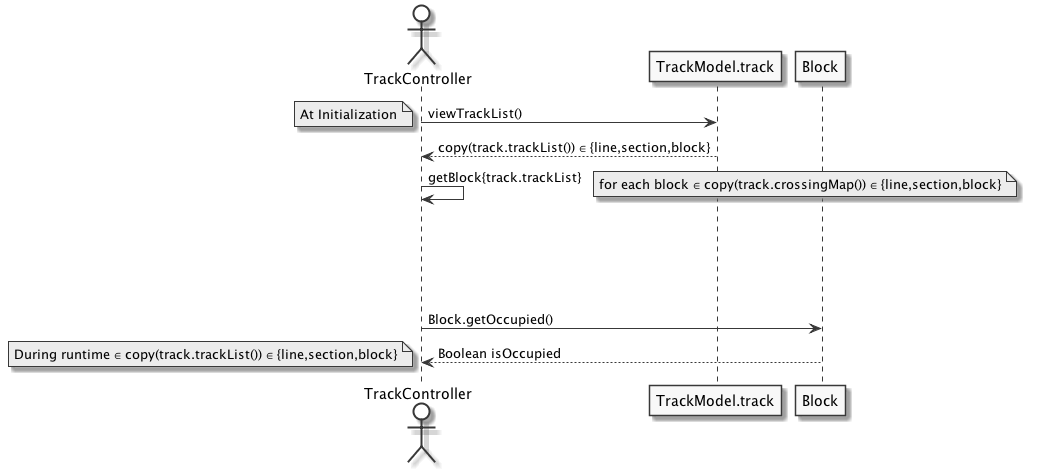
\includegraphics[width=\textwidth]{detectOccupied.png}
	\caption{Detect Block Occupancy Sequence Diagram}
\end{figure}
\begin{table}[H]
	\centering
	\caption{Detect block occupancy}
	\begin{tabular}{|l|l|}
		\hline
		Actors & \parbox[t]{10cm}{TrackController} \\ \hline
		Description & \parbox[t]{10cm}{The track controller iterates over the track to identify any occupied blocks} \\ \hline
		Data &  \parbox[t]{10cm}{None} \\ \hline
		Stimulus &  \parbox[t]{10cm}{None} \\ \hline
		Response & \parbox[t]{10cm}{None}\\ \hline
		Comments & \parbox[t]{10cm}{The TrackController is responsible for detecting block occupancy}  \\ \hline
	\end{tabular}
\end{table}

\begin{figure}[H]
	\centering
	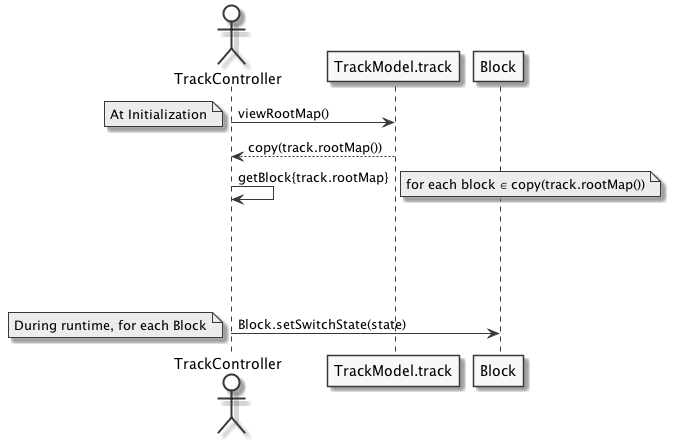
\includegraphics[scale=.5]{switching.png}
	\caption{Toggle Switching Sequence Diagram}
\end{figure}
\begin{table}[H]
	\centering
	\caption{Toggle switching use case description}
	\begin{tabular}{|l|l|}
		\hline
		Actors & \parbox[t]{10cm}{TrackController} \\ \hline
		Description & \parbox[t]{10cm}{The track controller switches track switches} \\ \hline
		Data &  \parbox[t]{10cm}{Boolean state of the switches of the track} \\ \hline
		Stimulus &  \parbox[t]{10cm}{The Track Controller calling the functions} \\ \hline
		Response & \parbox[t]{10cm}{Switching to the desired state}\\ \hline
		Comments & \parbox[t]{10cm}{The TrackController is expected to store the location of the switches at initialization}  \\ \hline
	\end{tabular}
\end{table}

\begin{figure}[H]
	\centering
	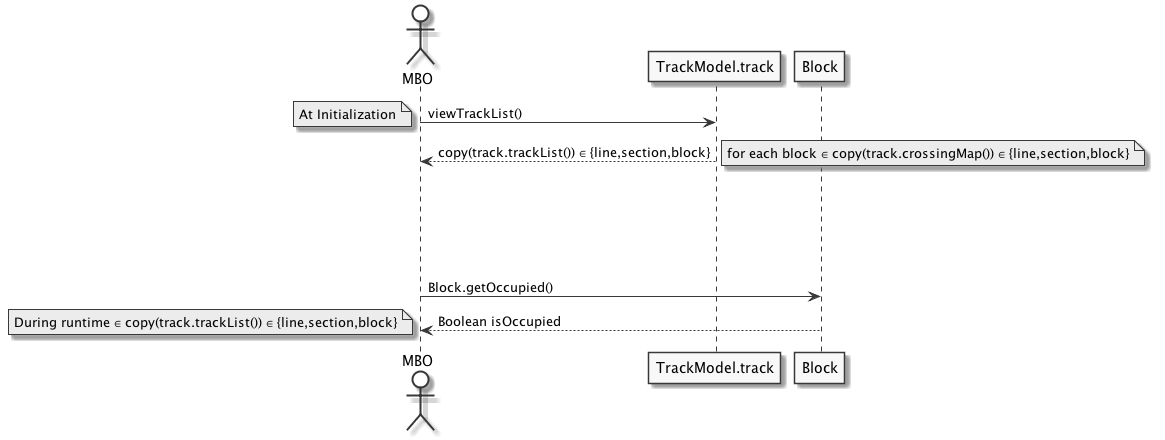
\includegraphics[width=\textwidth]{viewBlockOccupancy.png}
	\caption{View Block Occupancy Sequence Diagram}
\end{figure}

\begin{table}[H]
	\centering
	\caption{View Block occupancy}
	\begin{tabular}{|l|l|}
		\hline
		Actors & \parbox[t]{10cm}{MBO} \\ \hline
		Description & \parbox[t]{10cm}{The MBO views block occupancy when operating in MBO mode} \\ \hline
		Data &  \parbox[t]{10cm}{None} \\ \hline
		Stimulus &  \parbox[t]{10cm}{The MBO calling the track model} \\ \hline
		Response & \parbox[t]{10cm}{Return the occupancy state of the blocks in the track}\\ \hline
		Comments & \parbox[t]{10cm}{The MBO is expected to store the listing of blocks at initialization}  \\ \hline
	\end{tabular}
\end{table}

\begin{figure}[H]
	\centering
	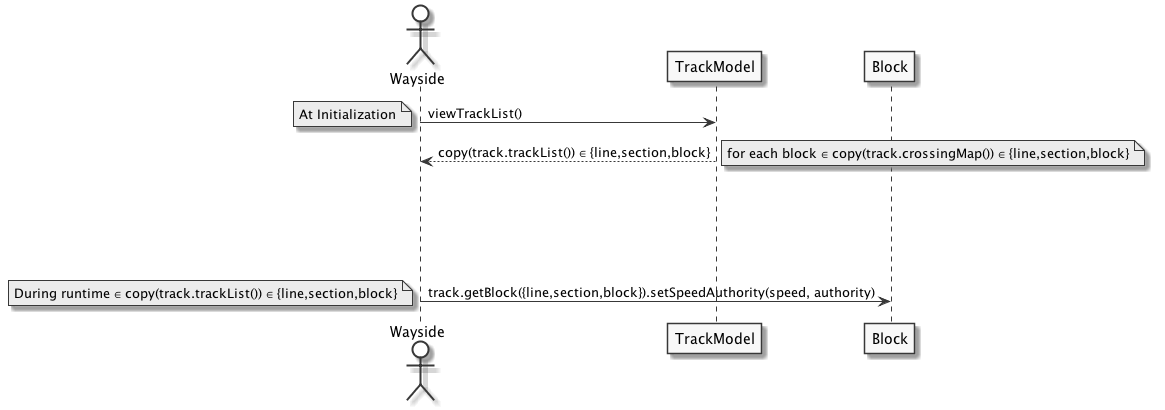
\includegraphics[width=\textwidth]{setSpeedAuthority.png}
	\caption{Set Speed and Authority Sequence Diagram}
\end{figure}
\begin{table}[H]
	\centering
	\caption{Set speed and authority description}
	\begin{tabular}{|l|l|}
		\hline
		Actors & \parbox[t]{10cm}{TrackController} \\ \hline
		Description & \parbox[t]{10cm}{The TrainController sets a given speed and authority at a block} \\ \hline
		Data &  \parbox[t]{10cm}{Double Speed, Block Authority} \\ \hline
		Stimulus &  \parbox[t]{10cm}{The TrainController calling the track model} \\ \hline
		Response & \parbox[t]{10cm}{Updating the communicated values of speed and authority sent by a given block}\\ \hline
		Comments & \parbox[t]{10cm}{The TrainController is expected to clear these values after use}  \\ \hline
	\end{tabular}
\end{table}

\begin{figure}[H]
	\centering
	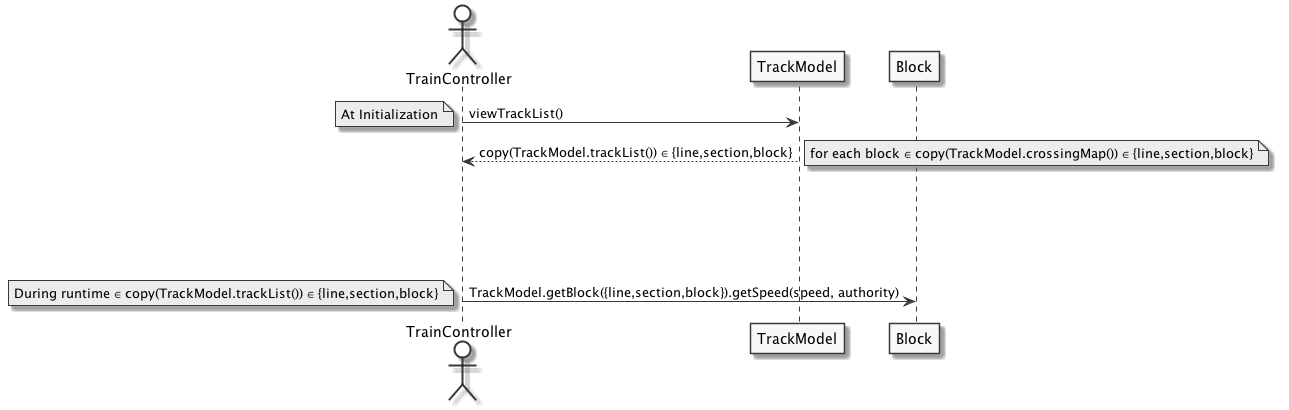
\includegraphics[width=\textwidth]{getSpeed.png}
	\caption{Get Speed Sequence Diagram}
\end{figure}

\begin{table}[H]
	\centering
	\caption{View speed}
	\begin{tabular}{|l|l|}
		\hline
		Actors & \parbox[t]{10cm}{TrainController} \\ \hline
		Description & \parbox[t]{10cm}{The TrainController views block speed message} \\ \hline
		Data &  \parbox[t]{10cm}{None} \\ \hline
		Stimulus &  \parbox[t]{10cm}{The TrainController calling the track model} \\ \hline
		Response & \parbox[t]{10cm}{Return the speed set at the block on the track}\\ \hline
		Comments & \parbox[t]{10cm}{This value is set by the TrainController}  \\ \hline
	\end{tabular}
\end{table}

\begin{figure}[H]
	\centering
	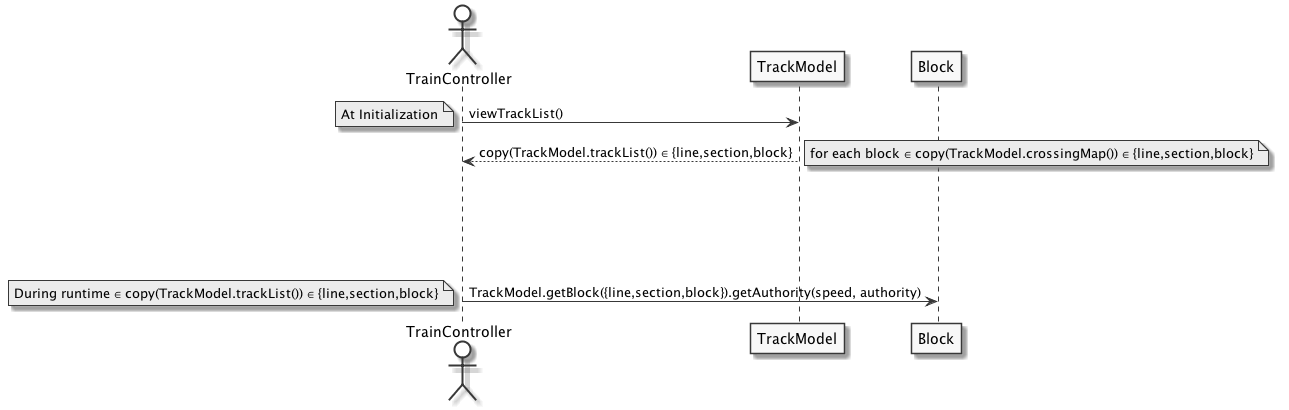
\includegraphics[width=\textwidth]{getAuthority.png}
	\caption{Get Authority Sequence Diagram}
\end{figure}
\begin{table}[H]
	\centering
	\caption{View authority}
	\begin{tabular}{|l|l|}
		\hline
		Actors & \parbox[t]{10cm}{TrainController} \\ \hline
		Description & \parbox[t]{10cm}{The TrainController views block authority message} \\ \hline
		Data &  \parbox[t]{10cm}{None} \\ \hline
		Stimulus &  \parbox[t]{10cm}{The TrainController calling the track model} \\ \hline
		Response & \parbox[t]{10cm}{Return the authority set at the block on the track}\\ \hline
		Comments & \parbox[t]{10cm}{This value is set by the TrainController}  \\ \hline
	\end{tabular}
\end{table}

\begin{figure}[H]
	\centering
	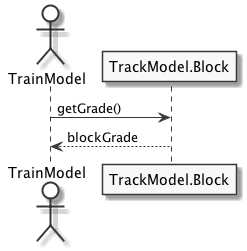
\includegraphics[scale=.5]{getGrade.png}
	\caption{Get Grade Sequence Diagram}
\end{figure}

\begin{table}[H]
	\centering
	\caption{View block grade}
	\begin{tabular}{|l|l|}
		\hline
		Actors & \parbox[t]{10cm}{TrainModel} \\ \hline
		Description & \parbox[t]{10cm}{The TrainModel views block grade attribute} \\ \hline
		Data &  \parbox[t]{10cm}{None} \\ \hline
		Stimulus &  \parbox[t]{10cm}{The TrainModel calling the track model} \\ \hline
		Response & \parbox[t]{10cm}{Return the grade read in at the block on the track}\\ \hline
		Comments & \parbox[t]{10cm}{This value is set at initialization}  \\ \hline
	\end{tabular}
\end{table}

\begin{figure}[H]
	\centering
	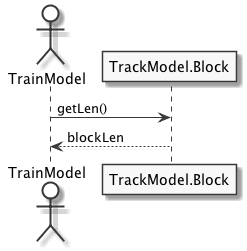
\includegraphics[scale=.5]{getLen.png}
	\caption{Get Length Sequence Diagram}
\end{figure}
\begin{table}[H]
	\centering
	\caption{View block length}
	\begin{tabular}{|l|l|}
		\hline
		Actors & \parbox[t]{10cm}{TrainModel} \\ \hline
		Description & \parbox[t]{10cm}{The TrainModel views block length attribute} \\ \hline
		Data &  \parbox[t]{10cm}{None} \\ \hline
		Stimulus &  \parbox[t]{10cm}{The TrainModel calling the track model} \\ \hline
		Response & \parbox[t]{10cm}{Return the length read in at the block on the track}\\ \hline
		Comments & \parbox[t]{10cm}{This value is set at initialization}  \\ \hline
	\end{tabular}
\end{table}

\begin{figure}[H]
	\centering
	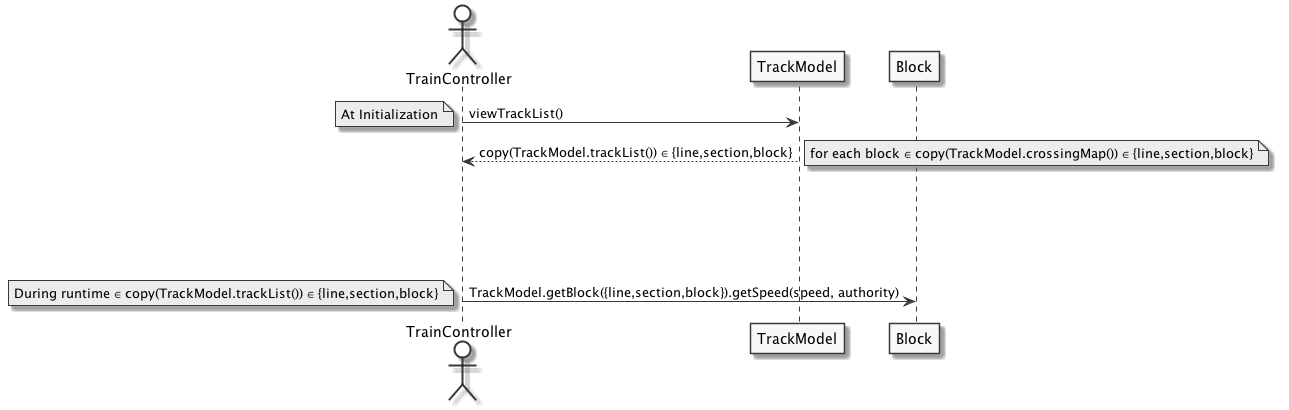
\includegraphics[width=\textwidth]{getSpeed.png}
	\caption{Get Speed Sequence Diagram}
\end{figure}
\begin{table}[H]
	\centering
	\caption{View block maximum speed}
	\begin{tabular}{|l|l|}
		\hline
		Actors & \parbox[t]{10cm}{TrainController} \\ \hline
		Description & \parbox[t]{10cm}{The TrainModel views block speed maximum setting read in at initialization} \\ \hline
		Data &  \parbox[t]{10cm}{None} \\ \hline
		Stimulus &  \parbox[t]{10cm}{The TrainModel calling the track model} \\ \hline
		Response & \parbox[t]{10cm}{Return the max block speed read in at the block on the track}\\ \hline
		Comments & \parbox[t]{10cm}{This value is set at initialization}  \\ \hline
	\end{tabular}
\end{table}

\begin{figure}[H]
	\centering
	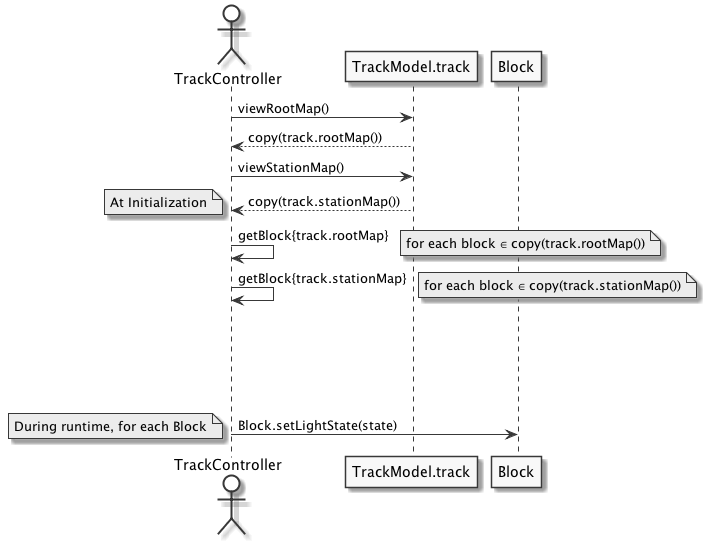
\includegraphics[width=\textwidth]{lights.png}
	\caption{Toggle Lights Sequence Diagram}
\end{figure}
\begin{table}[H]
	\centering
	\caption{Toggle block lights}
	\begin{tabular}{|l|l|}
		\hline
		Actors & \parbox[t]{10cm}{TrackController} \\ \hline
		Description & \parbox[t]{10cm}{The TrackModel toggles lights at any block that has them} \\ \hline
		Data &  \parbox[t]{10cm}{None} \\ \hline
		Stimulus &  \parbox[t]{10cm}{The TrackController calling the track model} \\ \hline
		Response & \parbox[t]{10cm}{Sets the lights to the boolean state passed by the TrackController (green=1,red=0)}\\ \hline
		Comments & \parbox[t]{10cm}{The TrackModel stores lights at each root of a switch and before and after a station}  \\ \hline
	\end{tabular}
\end{table}

\begin{figure}[H]
	\centering
	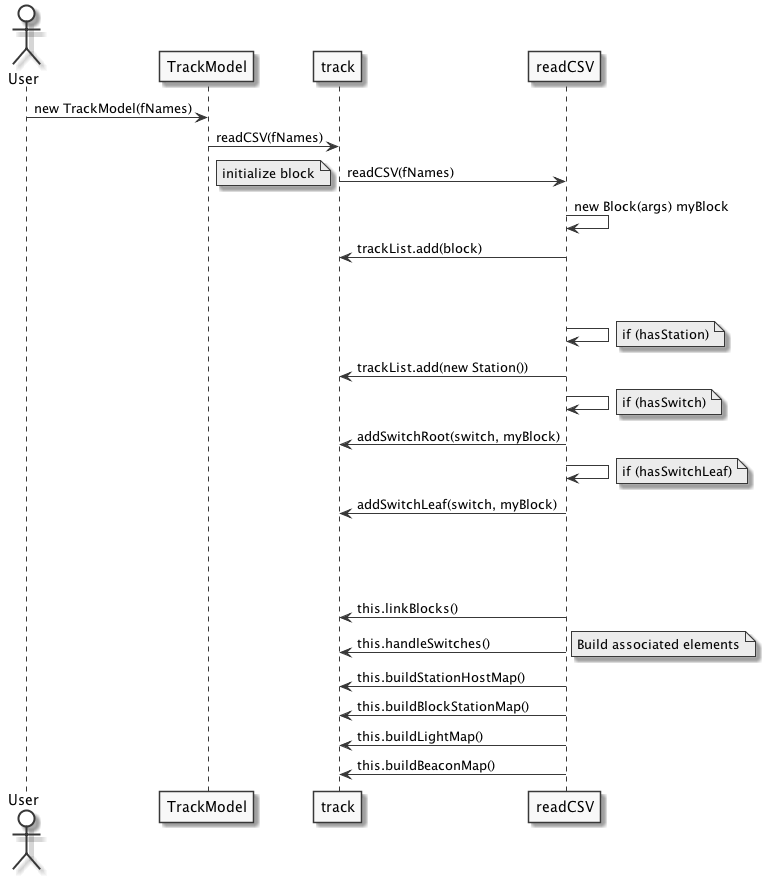
\includegraphics[scale=.5]{readFile.png}
	\caption{Read File Sequence Diagram}
\end{figure}

\begin{table}[H]
	\centering
	\caption{Read file}
	\begin{tabular}{|l|l|}
		\hline
		Actors & \parbox[t]{10cm}{User (train company)} \\ \hline
		Description & \parbox[t]{10cm}{The TrackModel CSV files to be read in} \\ \hline
		Data &  \parbox[t]{10cm}{CSV files for each file to be read in} \\ \hline
		Stimulus &  \parbox[t]{10cm}{The user starting the proram} \\ \hline
		Response & \parbox[t]{10cm}{The program will be run on those TrackModel}\\ \hline
		Comments & \parbox[t]{10cm}{The CSV functions are produced by Microsoft Excel :: Save As...::*.csv}  \\ \hline
	\end{tabular}
\end{table}

\begin{figure}[H]
	\centering
	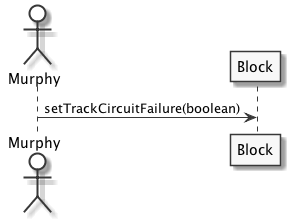
\includegraphics[scale=.5]{trackCircuitFailure.png}
	\caption{TrackCircuitFailure Test Case}
\end{figure}
\begin{table}[H]
	\centering
	\caption{Test Track Circuit Failure}
	\begin{tabular}{|l|l|}
		\hline
		Actors & \parbox[t]{10cm}{Murphy} \\ \hline
		Description & \parbox[t]{10cm}{The track circuit failure will no longer transmit after setting a failure state} \\ \hline
		Data &  \parbox[t]{10cm}{A boolean representing the failure states} \\ \hline
		Stimulus &  \parbox[t]{10cm}{A user seeking to test a track circuit failure} \\ \hline
		Response & \parbox[t]{10cm}{A track circuit failure}\\ \hline
		Comments & \parbox[t]{10cm}{This is concisdered a part of the testing and i snot a part of normal functionality}  \\ \hline
	\end{tabular}
\end{table}

\begin{figure}[H]
	\centering
	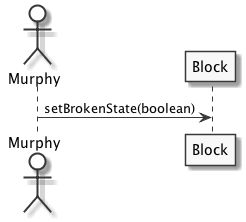
\includegraphics[scale=.5]{setBroken.png}
	\caption{TrackBrokenFailure Test Case}
\end{figure}
\begin{table}[H]
	\centering
	\caption{Test Track Broken Failure}
	\begin{tabular}{|l|l|}
		\hline
		Actors & \parbox[t]{10cm}{Murphy} \\ \hline
		Description & \parbox[t]{10cm}{The track block object broken state will be set for testing by this function} \\ \hline
		Data &  \parbox[t]{10cm}{A boolean representing the failure states} \\ \hline
		Stimulus &  \parbox[t]{10cm}{A user seeking to test a track block broken failure case} \\ \hline
		Response & \parbox[t]{10cm}{A track circuit broken setting}\\ \hline
		Comments & \parbox[t]{10cm}{This is concisdered a part of the testing and i snot a part of normal functionality}  \\ \hline
	\end{tabular}
\end{table}

\begin{figure}[H]
	\centering
	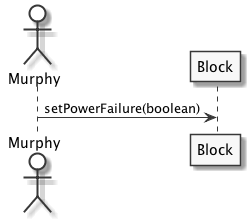
\includegraphics[scale=.5]{setPowerFailure.png}
	\caption{Track Power Failure Test Case}
\end{figure}
\begin{table}[H]
	\centering
	\caption{Test Track Power Failure}
	\begin{tabular}{|l|l|}
		\hline
		Actors & \parbox[t]{10cm}{Murphy} \\ \hline
		Description & \parbox[t]{10cm}{The track block object power failure state will be set for testing by this function} \\ \hline
		Data &  \parbox[t]{10cm}{A boolean representing the failure states} \\ \hline
		Stimulus &  \parbox[t]{10cm}{A user seeking to test a track block power failure case} \\ \hline
		Response & \parbox[t]{10cm}{A track power failure setting}\\ \hline
		Comments & \parbox[t]{10cm}{This is concisdered a part of the testing and i snot a part of normal functionality}  \\ \hline
	\end{tabular}
\end{table}

\subsection{Track Controller}
	\begin{figure}[H]
		\centering
		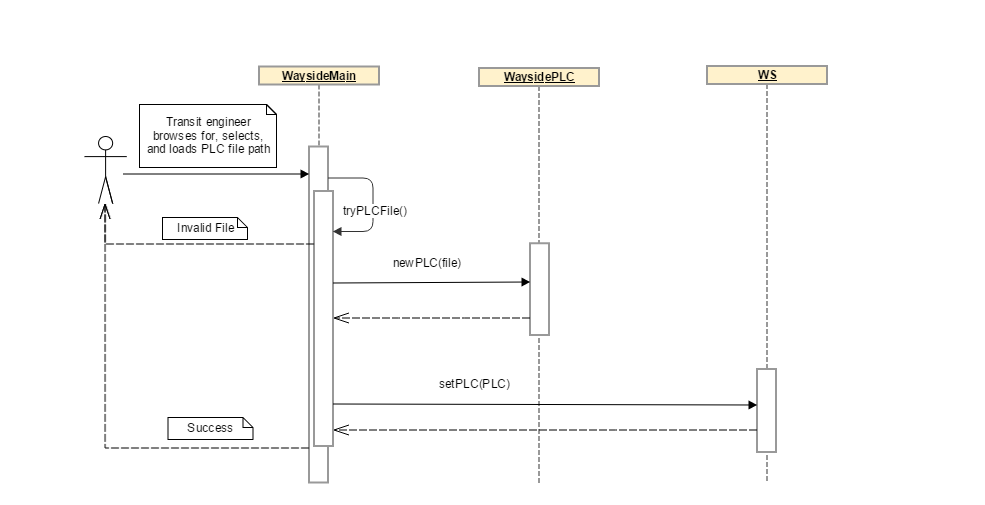
\includegraphics[scale=.5]{seq_wayside_loadplc.png}
		\caption{Loading a PLC file}
	\end{figure}
	\begin{table}[H]
		\centering
		\caption{Loading a PLC file}
		\begin{tabular}{|l|l|}
			\hline
			Actors & \parbox[t]{10cm}{Transit Engineer, Wayside Controller} \\ \hline
			Description & \parbox[t]{10cm}{The Transit Engineer browses for a PLC file and loads it. It is tested to make sure it is a valid file (Invalid File displayed if not valid), then a new PLC object is created and given to a WS (Wayside), and Success is displayed. } \\ \hline
			Data &  \parbox[t]{10cm}{PLC File} \\ \hline
			Stimulus &  \parbox[t]{10cm}{Loading of PLC File} \\ \hline
			Response & \parbox[t]{10cm}{File Evaluated and set}\\ \hline
			Comments & \parbox[t]{10cm}{The PLC file may be browsed for or the file path may simply be given}  \\ \hline
		\end{tabular}
	\end{table}
	
	\begin{figure}[H]
		\centering
		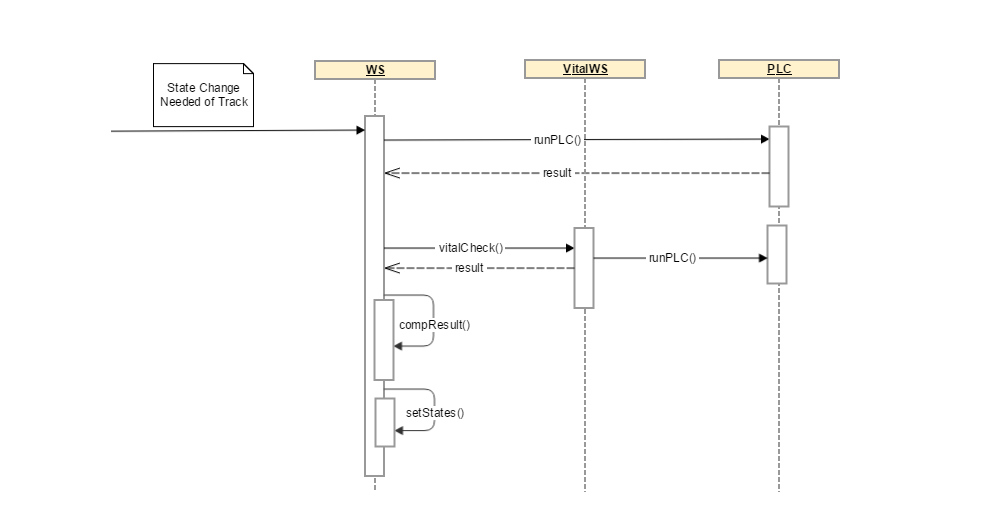
\includegraphics[scale=.5]{seq_wayside_setvital.png}
		\caption{Loading a PLC file}
	\end{figure}
	\begin{table}[H]
		\centering
		\caption{Vital Check}
		\begin{tabular}{|l|l|}
			\hline
			Actors & \parbox[t]{10cm}{Wayside Controller} \\ \hline
			Description & \parbox[t]{10cm}{When a change is needed on the Track, a Wayside Controller shall run its PLC code to determine if the change can be made and return a boolean result. This result will be compared with a sub-wayside unit which will evaluate the PLC code differently, and a result will be chosen to issue to the track. } \\ \hline
			Data &  \parbox[t]{10cm}{Switch, Light, or Crossing State} \\ \hline
			Stimulus &  \parbox[t]{10cm}{State Change needed} \\ \hline
			Response & \parbox[t]{10cm}{PLC Evaluation and Comparison, followed by changing track state if safe}\\ \hline
			Comments & \parbox[t]{10cm}{}  \\ \hline
		\end{tabular}
	\end{table}
	
	
	\begin{figure}[H]
		\centering
		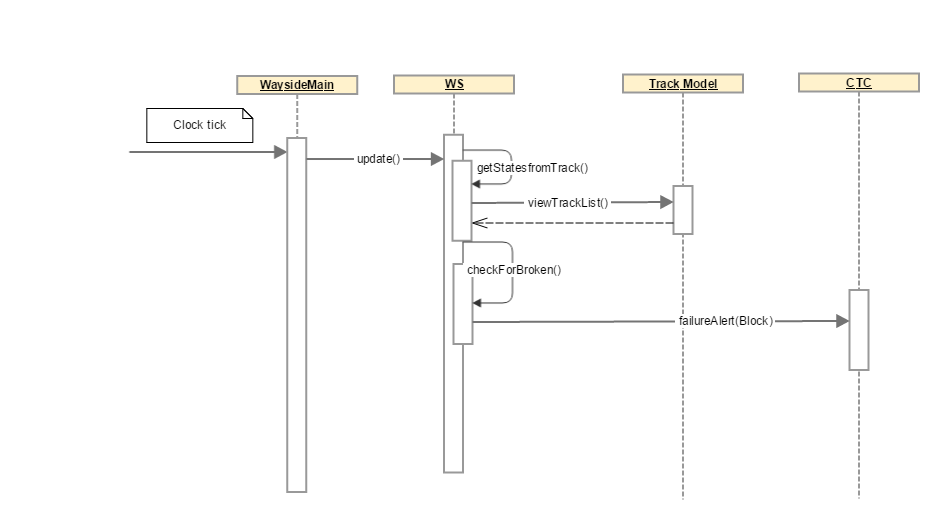
\includegraphics[scale=.5]{seq_wayside_updatetrack.png}
		\caption{Loading a PLC file}
	\end{figure}
	\begin{table}[H]
		\centering
		\caption{Update Track}
		\begin{tabular}{|l|l|}
			\hline
			Actors & \parbox[t]{10cm}{Wayside Controller, Track Model, CTC} \\ \hline
			Description & \parbox[t]{10cm}{The Wayside Controller will update its knowledge of the track every clock cycle. It shall retrieve the current state of track from the track model, and check for and report broken blocks to the CTC.} \\ \hline
			Data &  \parbox[t]{10cm}{Track State, Block} \\ \hline
			Stimulus &  \parbox[t]{10cm}{Clock tick} \\ \hline
			Response & \parbox[t]{10cm}{Track state retrieved, checked for broken blocks, report to CTC if any are broken.}\\ \hline
			Comments & \parbox[t]{10cm}{}  \\ \hline
		\end{tabular}
	\end{table}

\subsection{Train Model}
In this seciton, we provide the sequence diagrams of the train model.
\begin{figure}[H]
	\centering
	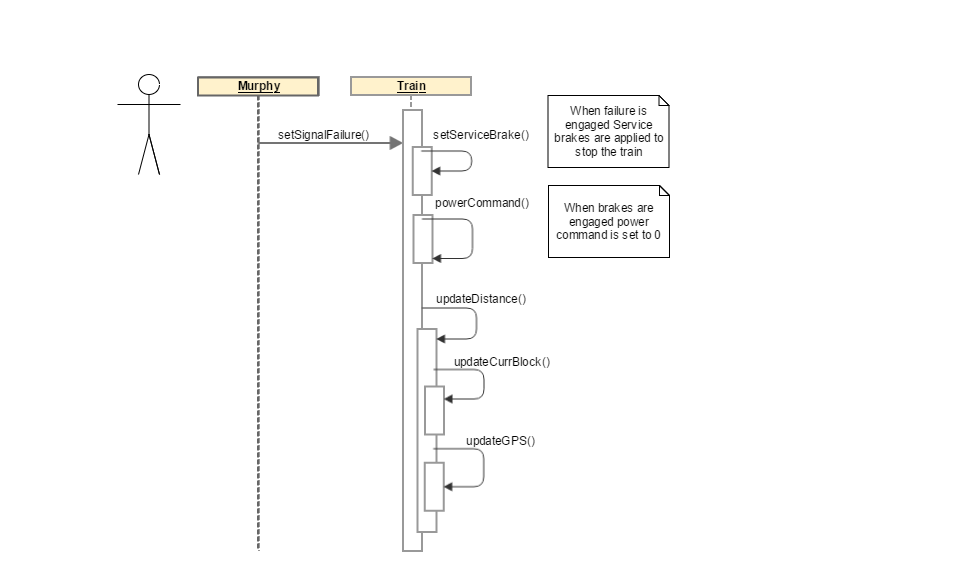
\includegraphics[scale=.5]{train_model_sqd_toggle_signal_failure.png}
	\caption{Toggle Signal Failure Sequence Diagram}
\end{figure}

\begin{table}[H]
	\centering
	\caption{Sequence Diagram for : Toggle Signal Failure}
	\begin{tabular}{|l|l|}
		\hline
		Actors & \parbox[t]{10cm}{Murphy, Train} \\ \hline
		Description & \parbox[t]{10cm}{Murphy is able to toggle the signal failure status in order to distrupt the train's signaling and communication abilities. Once engaged the train will be required to stop until the issue is resolved. In order to stop the service brake will be activated and this will send a power command of zero so that the train decelerates and the service brake rate. The current speed, distance, and location will all be updated as a result of the power command call.} \\ \hline
		Data &  \parbox[t]{10cm}{Signal Failure command, Service Brake Command} \\ \hline
		Stimulus &  \parbox[t]{10cm}{A command will be sent to the train model from the Murphy console to toggle the failure status of the train's signaling system.} \\ \hline
		Response & \parbox[t]{10cm}{The signal failure status will be toggled as a response to the command. When a signal failure occurs the service brakes are also engaged to bring the train to a stop until issues are resolved.}\\ \hline
		Comments & \parbox[t]{10cm}{The signal failure status will toggle between failure, and non-failure.}  \\ \hline
	\end{tabular}
\end{table}

\begin{figure}[H]
	\centering
	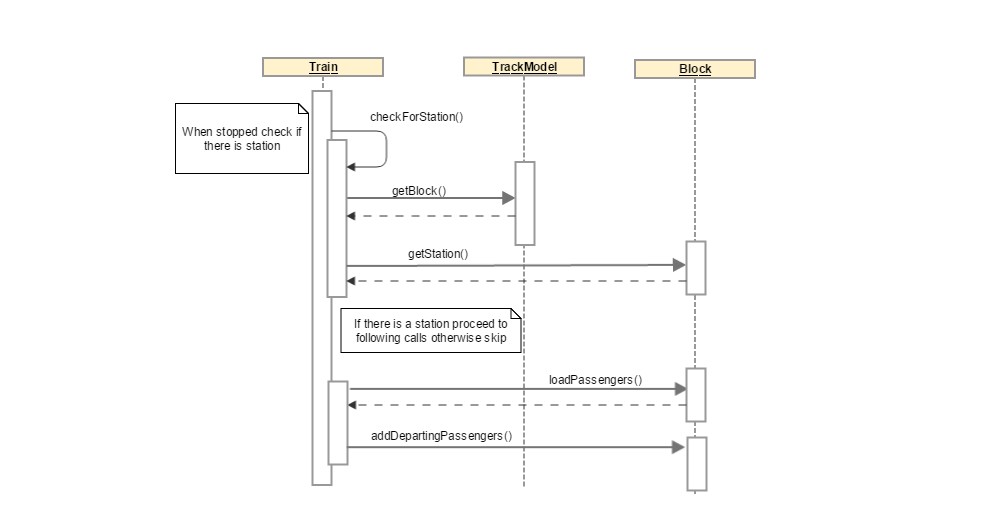
\includegraphics[scale=.5]{train_model_sqd_add_passengers.png}
	\caption{Add Passengers Sequence Diagram}
\end{figure}

\begin{table}[H]
	\centering
	\caption{Sequence Diagram for : checking for station}
	\begin{tabular}{|l|l|}
		\hline
		Actors & \parbox[t]{10cm}{Train, TrackModel, Block} \\ \hline
		Description & \parbox[t]{10cm}{Whenever stopped the train will check if it is stopped at a station. If there is a station, the train will request the actual block object from the TrackModel and using the block it will obtain a station object to add passengers from station onto the train and remove passengers from the train to the station.} \\ \hline
		Data &  \parbox[t]{10cm}{Current Block, Station, Passengers to Add, Passengers to remove} \\ \hline
		Stimulus &  \parbox[t]{10cm}{This check will occur every time the train comes to a complete stop} \\ \hline
		Response & \parbox[t]{10cm}{Current station will be returned and the number of passengers to add and remove will be determined}\\ \hline
		Comments & \parbox[t]{10cm}{ }  \\ \hline
	\end{tabular}
\end{table}

\begin{figure}[H]
	\centering
	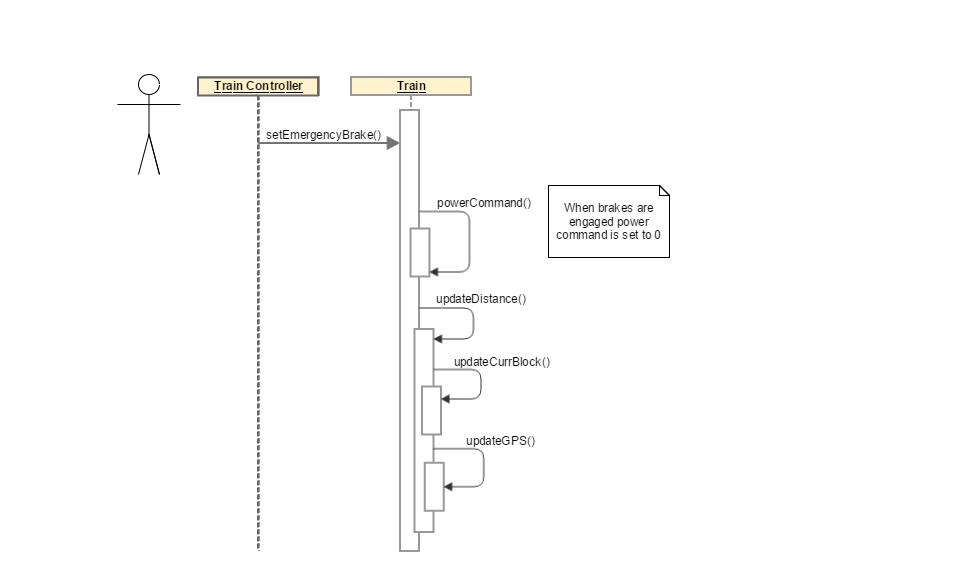
\includegraphics[scale=.5]{train_model_sqd_engage_emergency_brake.png}
	\caption{Engage Emergency Brake Sequence Diagram}
\end{figure}

	\begin{table}[H]
	\centering
	\caption{Sequence Diagram for : Engaging Emergency Brake}
	\begin{tabular}{|l|l|}
		\hline
		Actors & \parbox[t]{10cm}{Train Controller, Train} \\ \hline
		Description & \parbox[t]{10cm}{Train controller will engage or disengage the emergency brake in order to slow down or stop the train for any emergencies that may occur. Once engaged the power command will be set to zero and the train will begin to decelerate. The current speed, distance, and location will also be updated during the power command call.} \\ \hline
		Data &  \parbox[t]{10cm}{Emergency Brake command } \\ \hline
		Stimulus &  \parbox[t]{10cm}{Emergency brake will be engaged under the following conditions:\\1) Emergency brake button is manually pressed by the driver or passenger via the train controller\\2) Failure occurs in the service brakes and the emergency brakes are required to stop the train  } \\ \hline
		Response & \parbox[t]{10cm}{Emergency brake status is set to engaged and train begins to decelerate at emergency brake deceleration rate.}\\ \hline
		Comments & \parbox[t]{10cm}{The Emergency brake can either posses the status of on or off. For this model we are assuming that the emergency brakes never fail}  \\ \hline
	\end{tabular}
\end{table}

\begin{figure}[H]
	\centering
	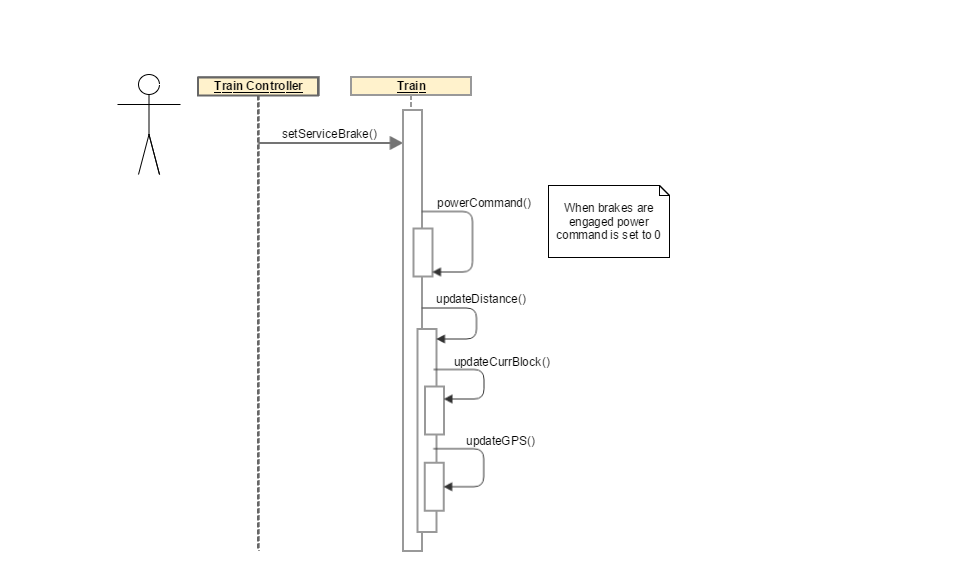
\includegraphics[scale=.5]{train_model_sqd_engage_service_brake.png}
	\caption{Engage Service Brake Sequence Diagram}
\end{figure}

\begin{table}[H]
	\centering
	\caption{Sequence Diagram for : Engaging Service Brake}
	\begin{tabular}{|l|l|}
		\hline
		Actors & \parbox[t]{10cm}{Train Controller, Train} \\ \hline
		Description & \parbox[t]{10cm}{Train controller will engage or disengage the Service brake in order to slow down or stop the train for any emergencies that may occur. Once engaged the power command will be set to zero and the train will begin to decelerate. The current speed, distance, and location will also be updated during the power command call.} \\ \hline
		Data &  \parbox[t]{10cm}{Service Brake command } \\ \hline
		Stimulus &  \parbox[t]{10cm}{Service brake will be engaged under the following conditions:\\1) Service brake button is manually pressed by the driver or passenger via the train controller\\2) Failure occurs in the engines or signaling and the Service brakes are required to stop the train  } \\ \hline
		Response & \parbox[t]{10cm}{Service brake status is set to engaged and train begins to decelerate at Service brake deceleration rate.}\\ \hline
		Comments & \parbox[t]{10cm}{The Service brake can either posses the status of on,off or failure}  \\ \hline
	\end{tabular}
\end{table}

\begin{figure}[H]
	\centering
	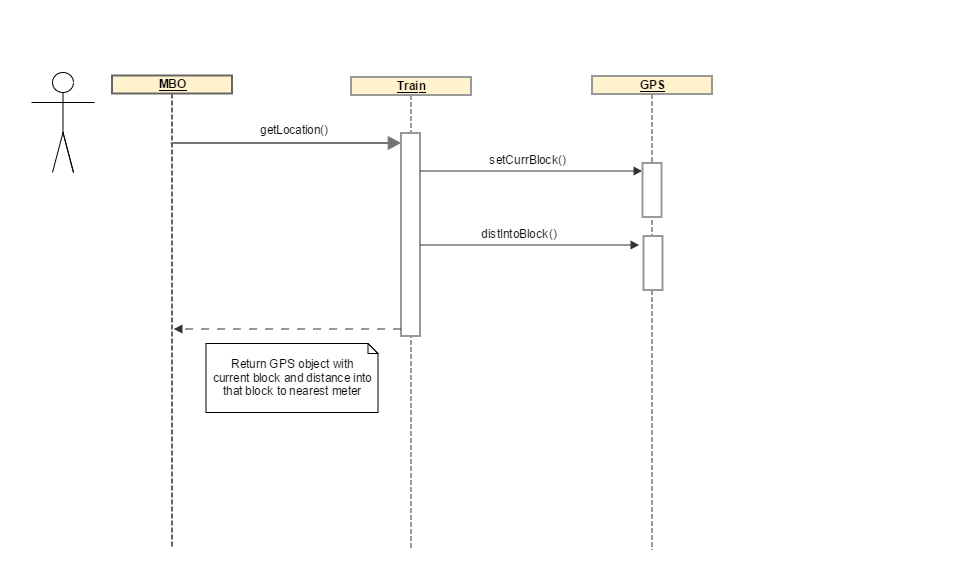
\includegraphics[scale=.3]{train_model_sqd_get_location.png}
	\caption{Get Location Sequence Diagram}
\end{figure}

\begin{table}[H]
	\centering
	\caption{Sequence Diagram for : Getting GPS Location}
	\begin{tabular}{|l|l|}
		\hline
		Actors & \parbox[t]{10cm}{MBO, Train} \\ \hline
		Description & \parbox[t]{10cm}{The MBO will request to receive the current location of the given train. This will be determined using the GPS object which is updated by the train calculations. The GPS object will be then returned to the MBO with the current block and distance into block to the nearest meter} \\ \hline
		Data &  \parbox[t]{10cm}{GPS position} \\ \hline
		Stimulus &  \parbox[t]{10cm}{Command will be requested from the MBO to get the current location from the train} \\ \hline
		Response & \parbox[t]{10cm}{GPS position object will be returned for that given train}\\ \hline
		Comments & \parbox[t]{10cm}{ }  \\ \hline
	\end{tabular}
\end{table}

\begin{figure}[H]
	\centering
	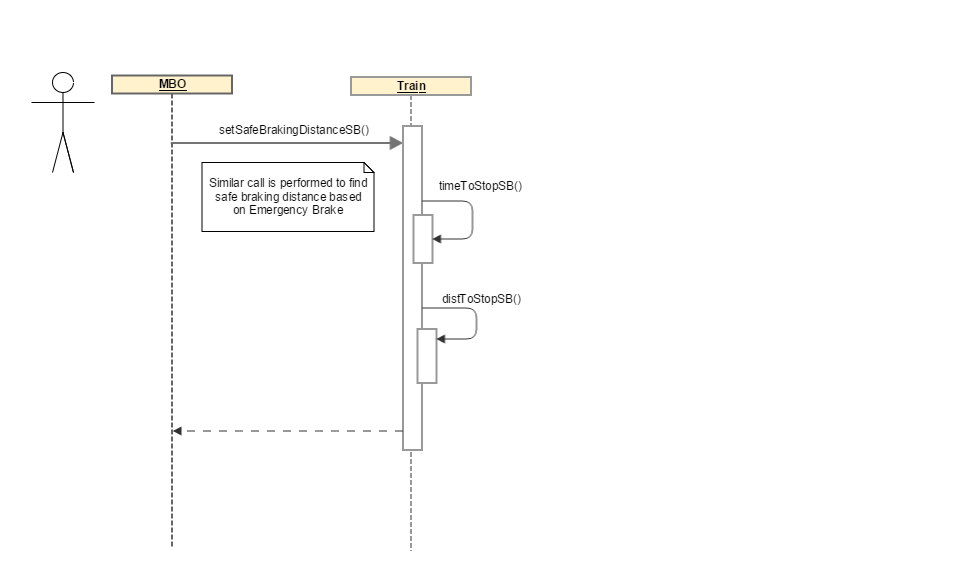
\includegraphics[scale=.5]{train_model_sqd_get_safebraking_dist.png}
	\caption{Calculate Safe Braking Distance Sequence Diagram}
\end{figure}

\begin{table}[H]
	\centering
	\caption{Sequence Diagram : Get Safe Braking Distance (Service Brake)}
	\begin{tabular}{|l|l|}
		\hline
		Actors & \parbox[t]{10cm}{MBO} \\ \hline
		Description & \parbox[t]{10cm}{In order to better determine the train's footprint the MBO will call to obtain the safe braking distance of the Train. This will be the distance required to bring the train to a complete stop using the service brake deceleration rate. This distance will vary based on the number of passengers on board the train and the current velocity of the train. The call will compute the time required to stop and based on current speed determine the distance required to stop. Similar procedure is performed for the safe braking distance using Emergency Brake} \\ \hline
		Data &  \parbox[t]{10cm}{Safe Braking Distance for Service Brake} \\ \hline
		Stimulus &  \parbox[t]{10cm}{Command will be requested from the MBO to get the current safe braking distance using the service brakes which would be computed based on the current velocity and mass of the train.} \\ \hline
		Response & \parbox[t]{10cm}{The safe braking distance using the service brakes will be returned to the MBO.}\\ \hline
		Comments & \parbox[t]{10cm}{ }  \\ \hline
	\end{tabular}
\end{table}

\begin{figure}[H]
	\centering
	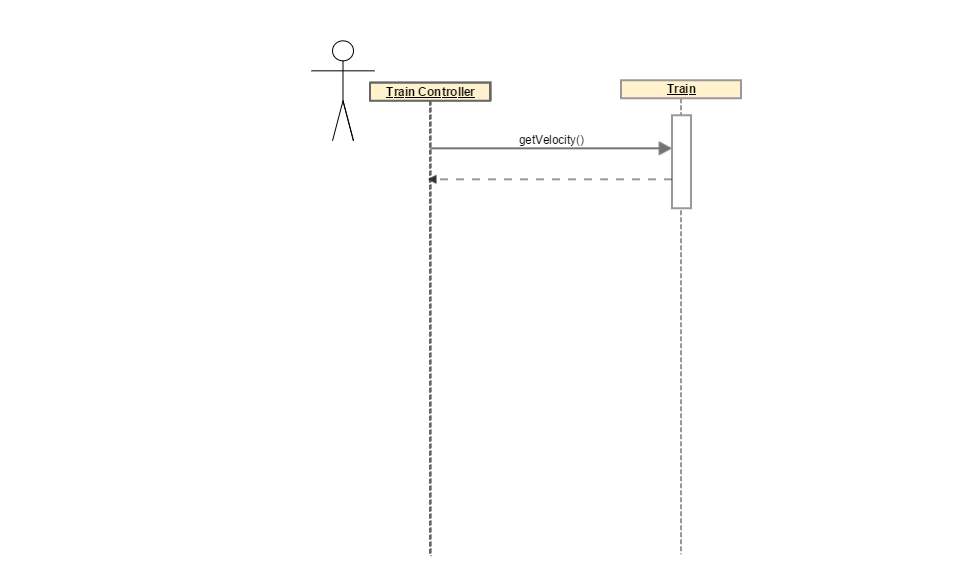
\includegraphics[scale=.5]{train_model_sqd_get_velocity.png}
	\caption{Get Velocity Sequence Diagram}
\end{figure}

\begin{table}[H]
	\centering
	\caption{Sequence Diagram for: Get Velocity}
	\begin{tabular}{|l|l|}
		\hline
		Actors & \parbox[t]{10cm}{Train Controller, Train} \\ \hline
		Description & \parbox[t]{10cm}{Train Controller will request the current velocity of the train periodically to modify the power command. Once requested the current velocity is returned to the Train Controller} \\ \hline
		Data &  \parbox[t]{10cm}{Get Velocity command  } \\ \hline
		Stimulus &  \parbox[t]{10cm}{The get velocity command is called by the train controller} \\ \hline
		Response & \parbox[t]{10cm}{The train will return its current velocity}\\ \hline
		Comments & \parbox[t]{10cm}{ }  \\ \hline
	\end{tabular}
\end{table}

\begin{figure}[H]
	\centering
	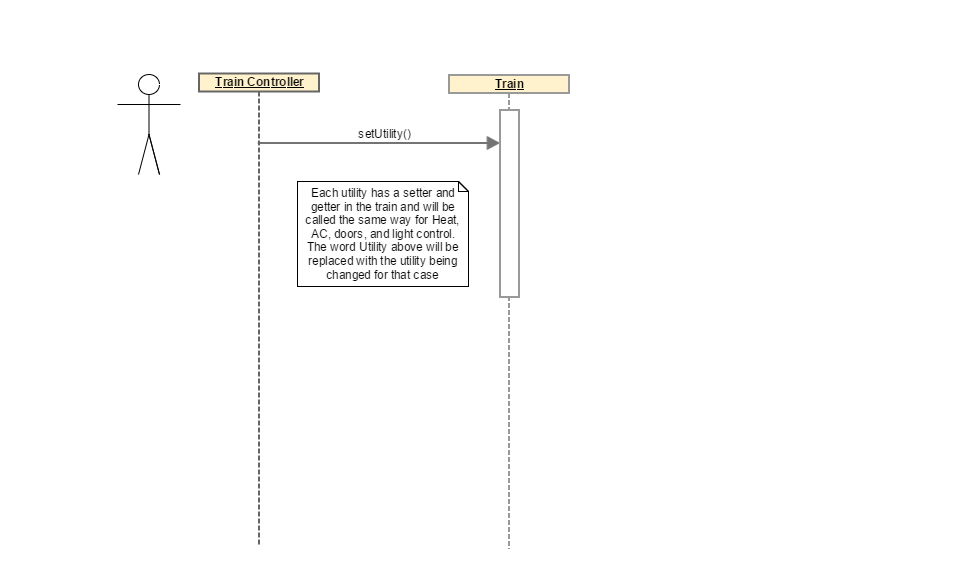
\includegraphics[scale=.5]{train_model_sqd_modify_utlilties.png}
	\caption{Modify Utilities Sequence Diagram}
\end{figure}

	\begin{table}[H]
	\centering
	\caption{Sequence Diagram for: Setting utilities}
	\begin{tabular}{|l|l|}
		\hline
		Actors & \parbox[t]{10cm}{Train Controller, Train} \\ \hline
		Description & \parbox[t]{10cm}{Each onboard train utility has a setter and getter for each train that the train controller will access to modify the selected utility. Similar commands will be used for the Heater, AC, Lights, and Door controls. } \\ \hline
		Data &  \parbox[t]{10cm}{Utility command } \\ \hline
		Stimulus &  \parbox[t]{10cm}{Setter is called to change the current status of a train utility} \\ \hline
		Response & \parbox[t]{10cm}{The status of the selected utility is changed to the corresponding value }\\ \hline
		Comments & \parbox[t]{10cm}{Each utility will be toggled individually and will require individual method calls to change each}  \\ \hline
	\end{tabular}
\end{table}

\begin{figure}[H]
	\centering
	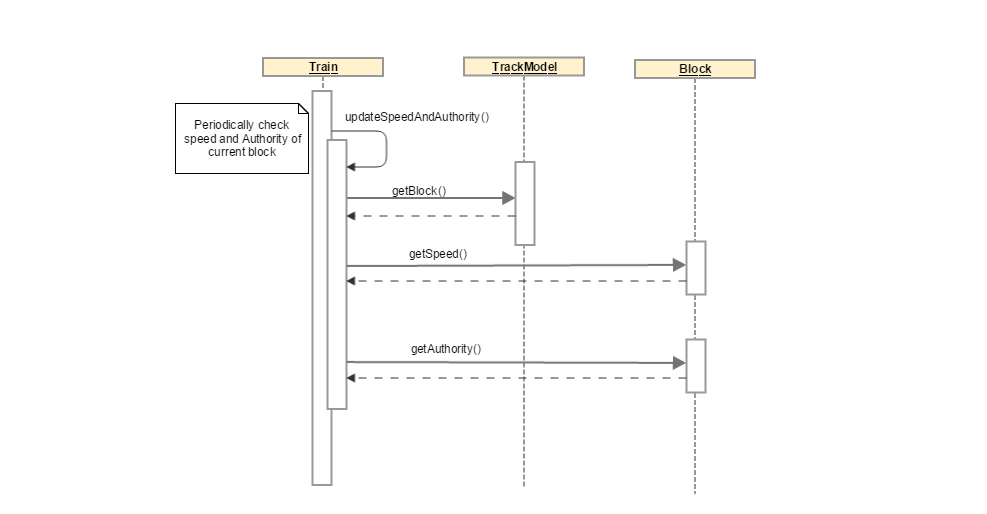
\includegraphics[scale=.5]{train_model_sqd_set_speed_authority.png}
	\caption{Set Speed and Authority Sequence Diagram}
\end{figure}

\begin{table}[H]
	\centering
	\caption{Sequence Diagram for: Updating Speed and Authority}
	\begin{tabular}{|l|l|}
		\hline
		Actors & \parbox[t]{10cm}{Train, Track Model, Block} \\ \hline
		Description & \parbox[t]{10cm}{Train will automatically check for updates on setpoint speed and authority from the track. This will be stored in the Track Model block objects. Using its current position the train will request the actual block object using the dummyBlock attributes. From that block object the setpoint speed and authority will be extracted to update the train values} \\ \hline
		Data &  \parbox[t]{10cm}{dummyBlock, currentBlock, Setpoint Speed, Authority } \\ \hline
		Stimulus &  \parbox[t]{10cm}{This check will occur periodically every clock tick in the system} \\ \hline
		Response & \parbox[t]{10cm}{The Setpoint speed and Authority will be updated based on the values dropped by the track model on the current block}\\ \hline
		Comments & \parbox[t]{10cm}{This method will only work in fixed mode. In MBO mode the speed and authority will be passed directly from the MBO to the train controller}  \\ \hline
	\end{tabular}
\end{table}

\begin{figure}[H]
	\centering
	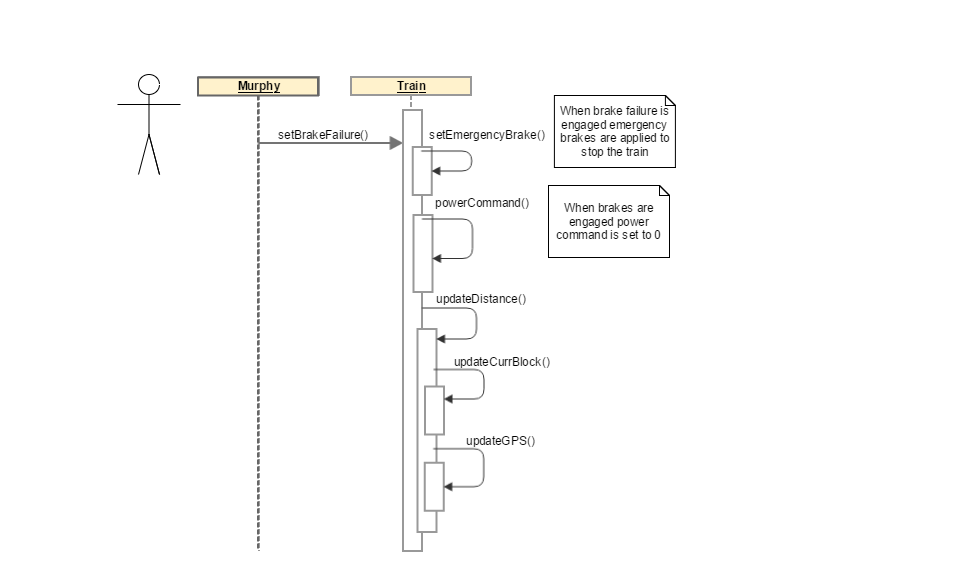
\includegraphics[scale=.5]{train_model_sqd_toggle_brake_failure.png}
	\caption{Toggle Brake Failure Sequence Diagram}
\end{figure}

	\begin{table}[H]
	\centering
	\caption{Sequence Diagram for : Toggle Brake Failure}
	\begin{tabular}{|l|l|}
		\hline
		Actors & \parbox[t]{10cm}{Murphy, Train} \\ \hline
		Description & \parbox[t]{10cm}{Murphy is able to toggle the brake failure status in order to distrupt the train's service brake. Once engaged the train will be required to stop until the issue is resolved. In order to stop the emergency brake will be activated and this will send a power command of zero so that the train decelerates and the emergency brake rate. The current speed, distance, and location will all be updated as a result of the power command call. } \\ \hline
		Data &  \parbox[t]{10cm}{Brake Failure command, Emergency Brake Command} \\ \hline
		Stimulus &  \parbox[t]{10cm}{A command will be sent to the train model from the Murphy console to toggle the failure status of the train's service brake. } \\ \hline
		Response & \parbox[t]{10cm}{The brake failure status will be toggled as a response to the command. When a service brake failure occurs the emergency brakes are also engaged to bring the train to a stop until issues are resolved.}\\ \hline
		Comments & \parbox[t]{10cm}{The brake failure status will toggle between failure, and non-failure.}  \\ \hline
	\end{tabular}
\end{table}

\begin{figure}[H]
	\centering
	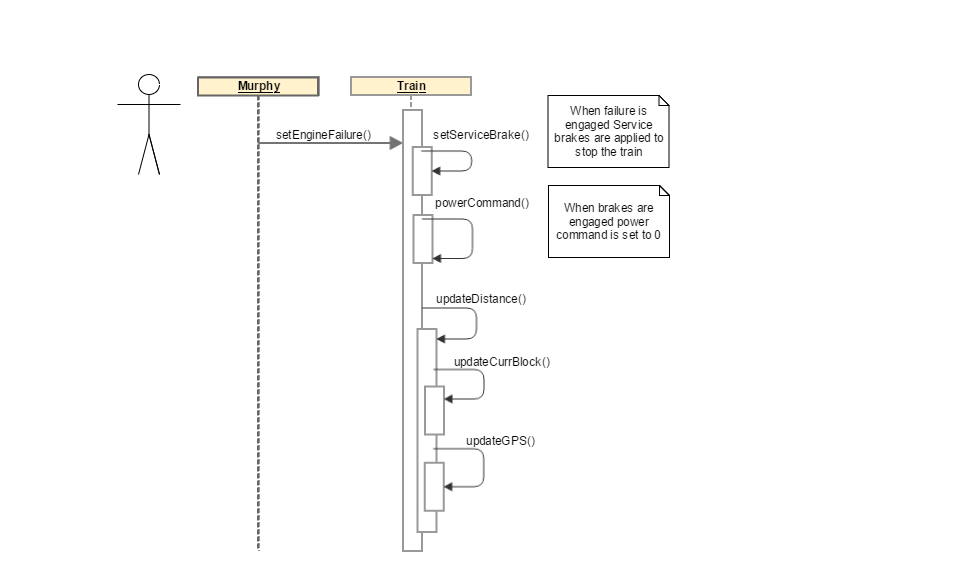
\includegraphics[scale=.5]{train_model_sqd_toggle_engine_failure.png}
	\caption{Toggle Engine Failure Sequence Diagram}
\end{figure}

\begin{table}[H]
	\centering
	\caption{Sequence Diagram for : Toggle Engine Failure}
	\begin{tabular}{|l|l|}
		\hline
		Actors & \parbox[t]{10cm}{Murphy} \\ \hline
		Description & \parbox[t]{10cm}{Murphy is able to toggle the engine failure status in order to distrupt the train's engine. Once engaged the train will be required to stop until the issue is resolved.In order to stop the service brake will be activated and this will send a power command of zero so that the train decelerates and the service brake rate. The current speed, distance, and location will all be updated as a result of the power command call.} \\ \hline
		Data &  \parbox[t]{10cm}{Engine Failure command, service Brake Command} \\ \hline
		Stimulus &  \parbox[t]{10cm}{A command will be sent to the train model from the Murphy console to toggle the failure status of the train's engine.} \\ \hline
		Response & \parbox[t]{10cm}{The engine failure status will be toggled as a response to the command. When an engine failure occurs the service brakes are also engaged to bring the train to a stop until issues are resolved.}\\ \hline
		Comments & \parbox[t]{10cm}{The engine failure status will toggle between failure, and non-failure. }  \\ \hline
	\end{tabular}
\end{table}

\begin{figure}[H]
	\centering
	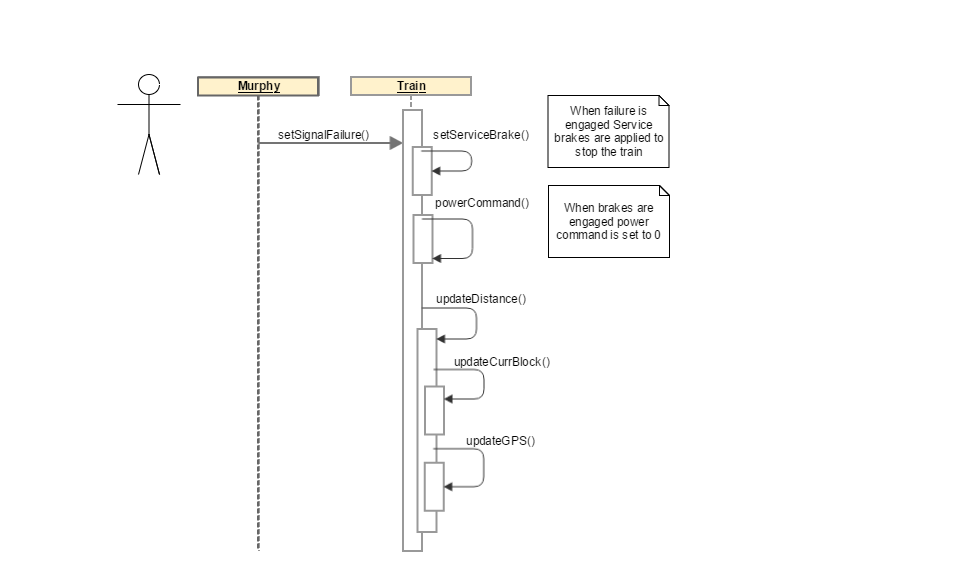
\includegraphics[scale=.5]{train_model_sqd_toggle_signal_failure.png}
	\caption{Toggle Signal Failure Sequence Diagram}
\end{figure}

\begin{table}[H]
	\centering
	\caption{Sequence Diagram for : Toggle Signal Failure}
	\begin{tabular}{|l|l|}
		\hline
		Actors & \parbox[t]{10cm}{Murphy, Train} \\ \hline
		Description & \parbox[t]{10cm}{Murphy is able to toggle the signal failure status in order to distrupt the train's signaling and communication abilities. Once engaged the train will be required to stop until the issue is resolved. In order to stop the service brake will be activated and this will send a power command of zero so that the train decelerates and the service brake rate. The current speed, distance, and location will all be updated as a result of the power command call.} \\ \hline
		Data &  \parbox[t]{10cm}{Signal Failure command, Service Brake Command} \\ \hline
		Stimulus &  \parbox[t]{10cm}{A command will be sent to the train model from the Murphy console to toggle the failure status of the train's signaling system.} \\ \hline
		Response & \parbox[t]{10cm}{The signal failure status will be toggled as a response to the command. When a signal failure occurs the service brakes are also engaged to bring the train to a stop until issues are resolved.}\\ \hline
		Comments & \parbox[t]{10cm}{The signal failure status will toggle between failure, and non-failure.}  \\ \hline
	\end{tabular}
\end{table}

\begin{figure}[H]
	\centering
	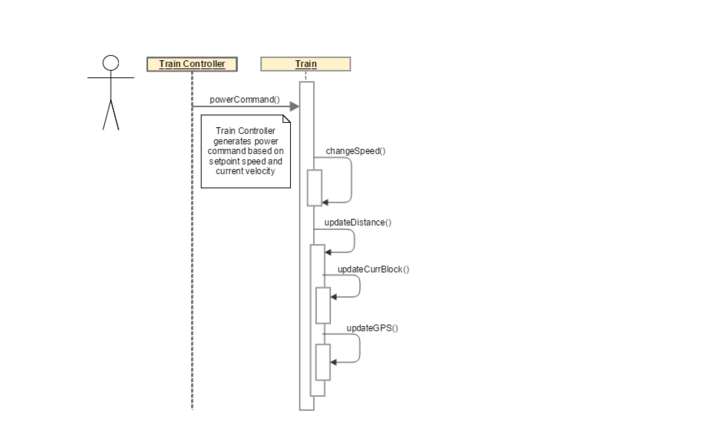
\includegraphics[scale=.5]{train_model_sqd_set_power.png}
	\caption{Toggle set Power Sequence Diagram}
\end{figure}

\begin{table}[H]
	\centering
	\caption{Sequence Diagram for : Set New Power Command}
	\begin{tabular}{|l|l|}
		\hline
		Actors & \parbox[t]{10cm}{Train Controller , Train} \\ \hline
		Description & \parbox[t]{10cm}{Train Controller will set a new power command based on the current velocity of the train and the new setpoint speed set by the driver. This power command will be used to determine the force applied to the train and thus compute the new current velocity. Using the new velocity the distance traveled by the train will be updated. This will be used to update the current block and GPS location for determining the Grade and current position} \\ \hline
		Data &  \parbox[t]{10cm}{Power Command issued to the train} \\ \hline
		Stimulus &  \parbox[t]{10cm}{When a setpoint speed is provided to the train controller, a Power command is computed using the current velocity and sent to train} \\ \hline
		Response & \parbox[t]{10cm}{New current velocity is computed by the train and using this new velocity, the distance traveled , current Block, and GPS position are all updated }\\ \hline
		Comments & \parbox[t]{10cm}{Power command sent must be between 0W and 120kW}  \\ \hline
	\end{tabular}
\end{table}

\subsection{Train Controller}

\begin{figure}[H]
	\centering
	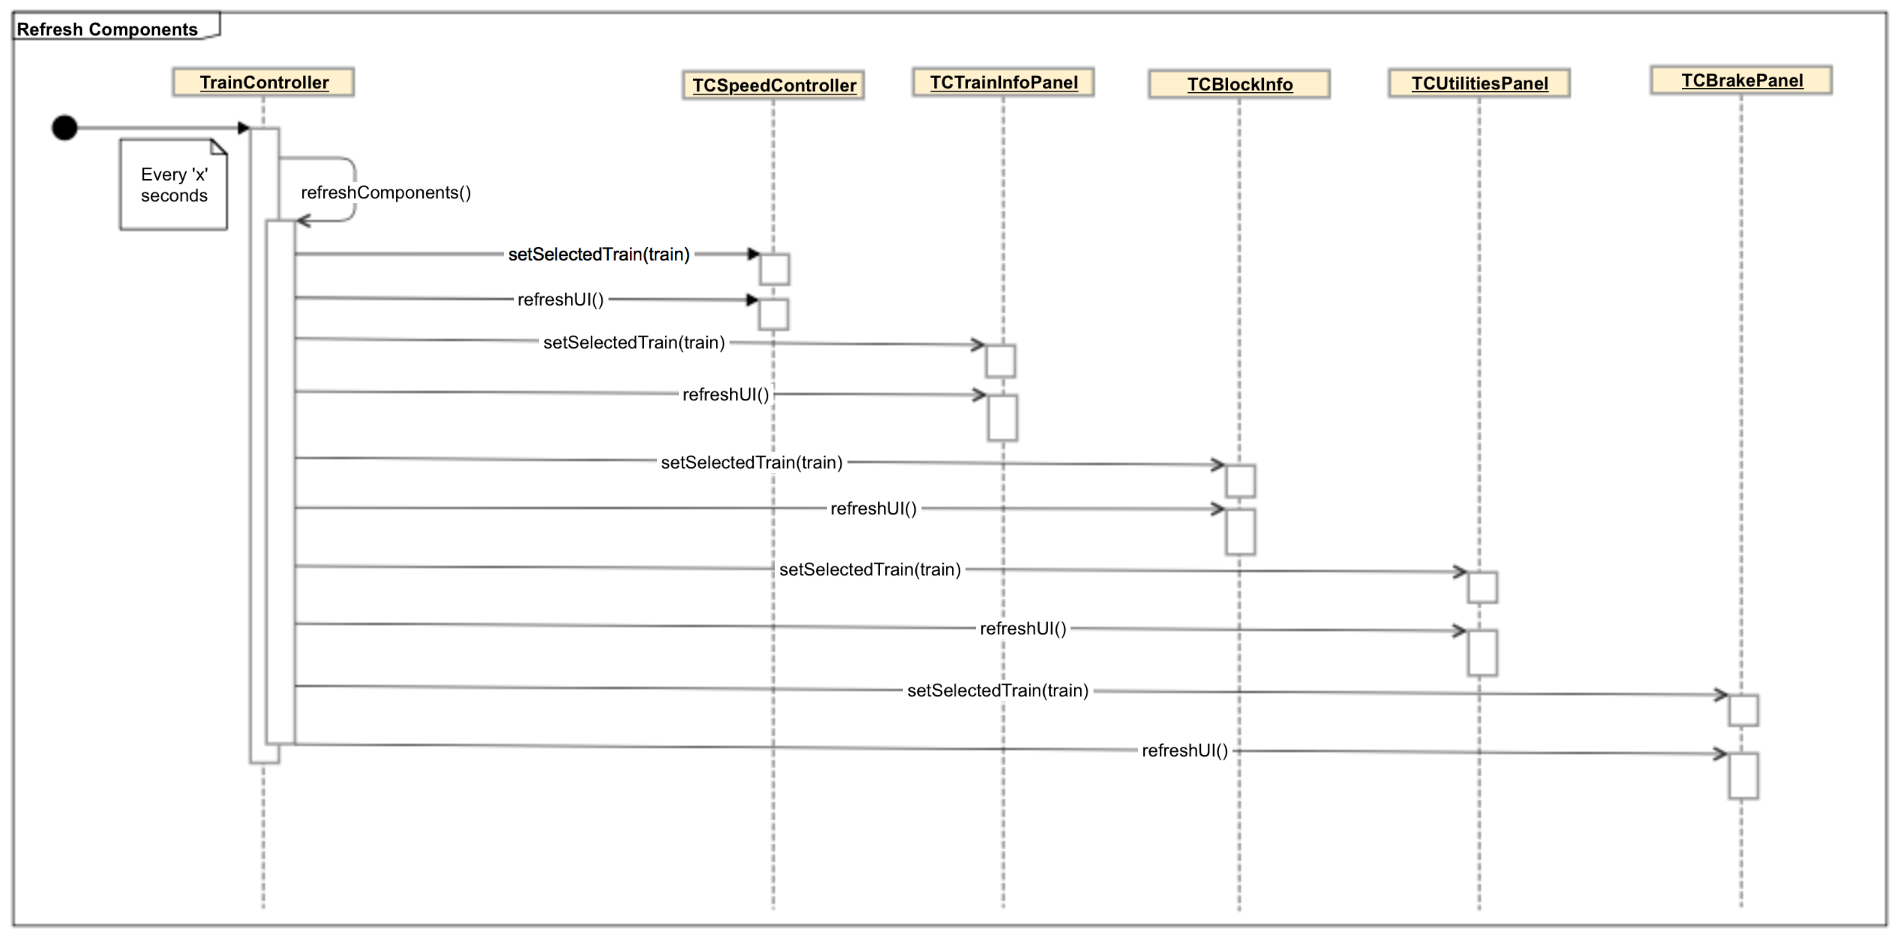
\includegraphics[width=\textwidth]{tc_refreshui_usecase}
	\caption{Refresh Components Sequence Diagram}
\end{figure}

\begin{table}[H]
	\centering
	\caption{Refresh Components}
	\begin{tabular}{|l|l|}
		\hline
		Actors & \parbox[t]{10cm}{TrainController, TCUtilitiesPanel, TCSpeedController, TCBlockInfo, TCBrakePanel, TCTrainInfoPanel} \\ \hline
		Description & \parbox[t]{10cm}{This method is called during every clock tick. It passes in the train the TrainController is controlling to its sub-components, and then refreshes each of the sub-components.} \\ \hline
		Data &  \parbox[t]{10cm}{The selected train} \\ \hline
		Stimulus &  \parbox[t]{10cm}{ Happens during every clock tick} \\ \hline
		Response & \parbox[t]{10cm}{The sub-components refresh their UI to reflect the train information of the passed in train. }\\ \hline
		Comments & \parbox[t]{10cm}{}  \\ \hline
	\end{tabular}
\end{table}

\begin{figure}[H]
	\centering
	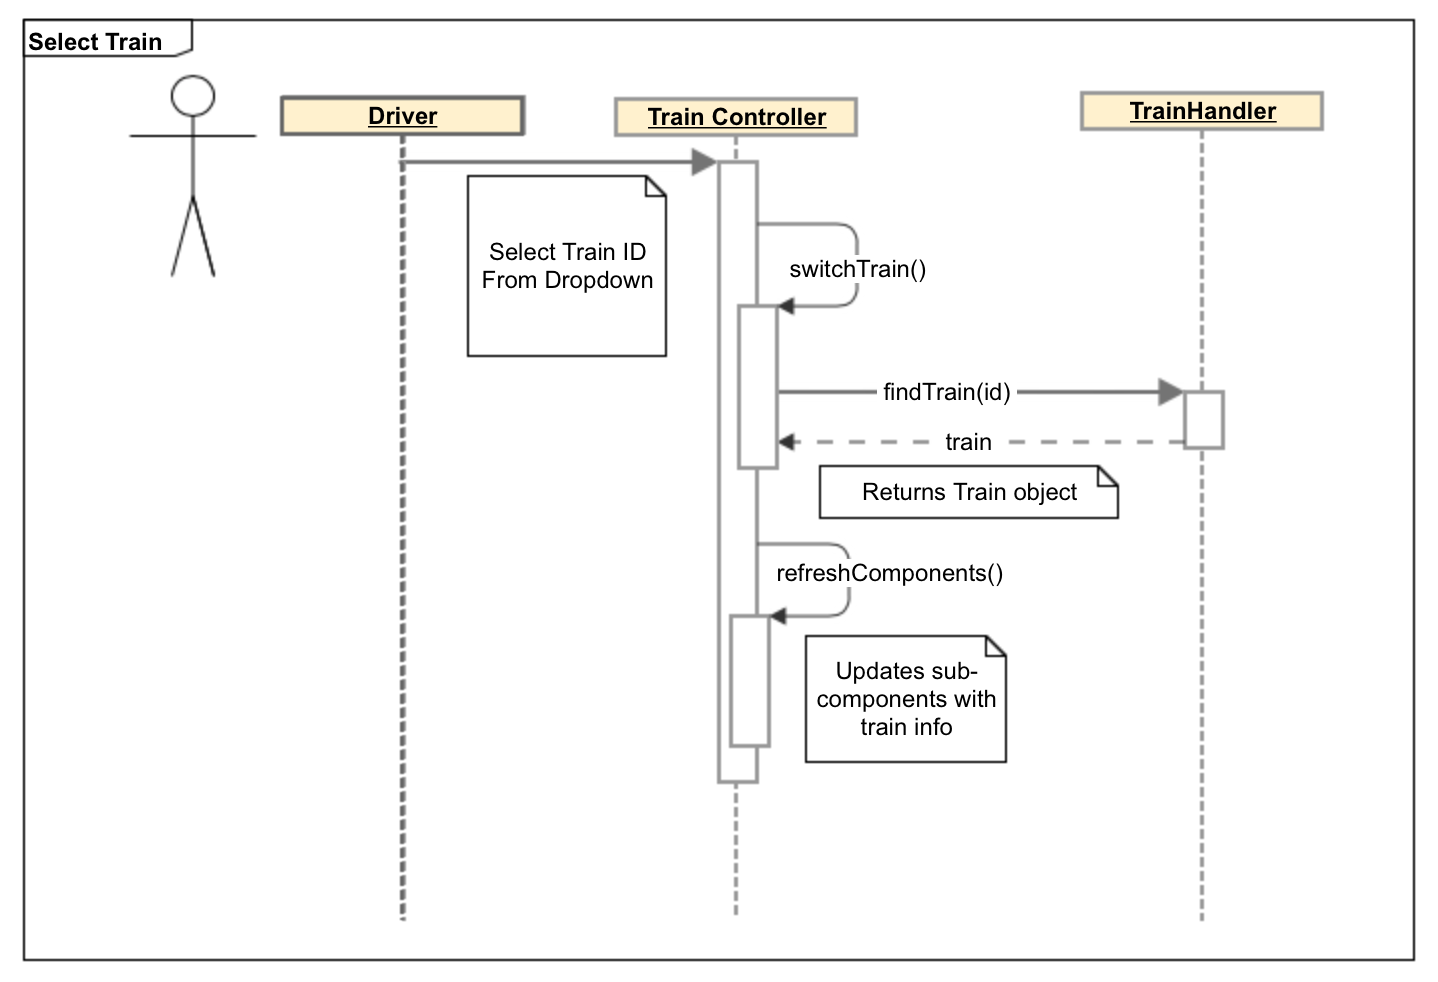
\includegraphics[width=\textwidth]{tc_selectTrain_usecase}
	\caption{Select Train Sequence Diagram}
\end{figure}

\begin{table}[H]
	\centering
	\caption{Select Train}
	\begin{tabular}{|l|l|}
		\hline
		Actors & \parbox[t]{10cm}{Driver, TrainHandler} \\ \hline
		Description & \parbox[t]{10cm}{The user picks a train from the list of dispatched trains to via the Train Controller. The user clicks the 'Switch'. The ID in the dropdown is sent to the TrainHandler and returns the train with the corresponding ID. The Train Controller then refreshes its components.} \\ \hline
		Data &  \parbox[t]{10cm}{Train ID} \\ \hline
		Stimulus &  \parbox[t]{10cm}{ A train was selected from the drop down and the 'Switch' button was pressed by the user. } \\ \hline
		Response & \parbox[t]{10cm}{Switches the train that the Train Controller is controlling and updates the sub-components of with the train information.  }\\ \hline
		Comments & \parbox[t]{10cm}{}  \\ \hline
	\end{tabular}
\end{table}


\begin{figure}[H]
	\centering
	\includegraphics[width=\textwidth]{tc_setKpAndKi_usecase}
	\caption{Set $K_p$ and $K_i$ Sequence Diagram}
\end{figure}

\begin{table}[H]
	\centering
	\caption{Set $K_p$ and $K_i$}
	\begin{tabular}{|l|l|}
		\hline
		Actors & \parbox[t]{10cm}{Engineer, Train, TCEngineerFrame} \\ \hline
		Description & \parbox[t]{10cm}{The user selects a for the Train Controller to control and switches to that train. If the selected train has no $K_p$ and $K_i$ set, the Engineer Frame opens. The Engineer can then set the $K_p$ and $K_i$. The user can also change the Kp and Ki by clicking the 'Set Kp/Ki' button. The train then has its $K_p$ and $K_i$ set.} \\ \hline
		Data &  \parbox[t]{10cm}{The selected train} \\ \hline
		Stimulus &  \parbox[t]{10cm}{ Happens when the user clicks the 'Set $K_p$/$K_i$' button or the user selects a train that has no $K_p$ and $K_i$ set. } \\ \hline
		Response & \parbox[t]{10cm}{Sets the $K_p$ and $K_i$ of the selected train.  }\\ \hline
		Comments & \parbox[t]{10cm}{}  \\ \hline
	\end{tabular}
\end{table}

\begin{figure}[H]
	\centering
	\includegraphics[width=\textwidth]{tc_speedAndAuth_usecase}
	\caption{Get Suggested Speed and Authority Sequence Diagram}
\end{figure}

\begin{table}[H]
	\centering
	\caption{Get Suggested Speed and Authority}
	\begin{tabular}{|l|l|}
		\hline
		Actors & \parbox[t]{10cm}{Train, TCBlockInfo, TCTrainInfoPanel} \\ \hline
		Description & \parbox[t]{10cm}{The Train Controller gets the suggested speed and authority from the selected train during every clock tick. The Train Controller then refreshes its components.} \\ \hline
		Data &  \parbox[t]{10cm}{The selected train} \\ \hline
		Stimulus &  \parbox[t]{10cm}{ This happens every clock tick. } \\ \hline
		Response & \parbox[t]{10cm}{The suggested speed and authority of the selected train is obtained and used to update the Train Info Pane and the Block Info Pane.  }\\ \hline
		Comments & \parbox[t]{10cm}{}  \\ \hline
	\end{tabular}
\end{table}

\begin{figure}[H]
	\centering
	\includegraphics[width=\textwidth]{tc_turnOnLights_usecase}
	\caption{Turn On Lights Sequence Diagram}
\end{figure}

\begin{table}[H]
	\centering
	\caption{Turn on Lights}
	\begin{tabular}{|l|l|}
		\hline
		Actors & \parbox[t]{10cm}{Driver, Train, TCUtilities, TrainController} \\ \hline
		Description & \parbox[t]{10cm}{The user turns on the lights by choosing the 'ON' radio button from the Utilities Panel or the system detects that the lights need to be turned on. This will tell the selected train to turn on its lights. On the next clock tick, the UI elements of the Utility Panel will be updated.} \\ \hline
		Data &  \parbox[t]{10cm}{The selected train} \\ \hline
		Stimulus &  \parbox[t]{10cm}{The user chooses the 'ON' radio button or the system detects that the lights must be turned on.  } \\ \hline
		Response & \parbox[t]{10cm}{The selected train turns on its lights. }\\ \hline
		Comments & \parbox[t]{10cm}{}  \\ \hline
	\end{tabular}
\end{table}

\begin{figure}[H]
	\centering
	\includegraphics[width=\textwidth]{tc_openDoors_usecase}
	\caption{Open Doors Sequence Diagram}
\end{figure}

\begin{table}[H]
	\centering
	\caption{Open Doors}
	\begin{tabular}{|l|l|}
		\hline
		Actors & \parbox[t]{10cm}{Driver, Train, TCUtilities, TrainController} \\ \hline
		Description & \parbox[t]{10cm}{The user changes the radio button of the specified doors by selecting the 'Open' radio button. This tells the selected train to open its doors. On the next clock tick, the UI is updated to reflect the state of the doors. If the system is in Automatic mode, and detects that the train must open its door (stopped at a station, etc..), this process is repeated without the user interaction.} \\ \hline
		Data &  \parbox[t]{10cm}{The selected train} \\ \hline
		Stimulus &  \parbox[t]{10cm}{ This happens when the user chooses the 'Open' radio button or the system needs to open the doors to let passengers in and out. } \\ \hline
		Response & \parbox[t]{10cm}{The doors on the train are opened. }\\ \hline
		Comments & \parbox[t]{10cm}{The doors can only be opened when the train is stopped. Assume that the train is stopped for the call diagram. }  \\ \hline
	\end{tabular}
\end{table}

\begin{figure}[H]
	\centering
	\includegraphics[width=\textwidth]{tc_turnOnAC_usecase}
	\caption{Turn On Air Conditioning Sequence Diagram}
\end{figure}

\begin{table}[H]
	\centering
	\caption{Turn on Air Conditioning}
	\begin{tabular}{|l|l|}
		\hline
		Actors & \parbox[t]{10cm}{Driver, Train, TCUtilities, TrainController} \\ \hline
		Description & \parbox[t]{10cm}{The user changes the radio button of the AC to 'On'. This tells the train to turn on its AC unit, and to turn off the heat. On the next clock tick, the UI elements are updated to reflect the state of the AC. If the system in in Automatic mode, and detects that the temperature is too high, this process is repeated without the user interaction. } \\ \hline
		Data &  \parbox[t]{10cm}{The selected train} \\ \hline
		Stimulus &  \parbox[t]{10cm}{ The user chooses the 'ON' radio button or the system detects that the temperature on the train is too high. } \\ \hline
		Response & \parbox[t]{10cm}{Turns on the AC and tells the train to set its temperature to the desired temperature.}\\ \hline
		Comments & \parbox[t]{10cm}{}  \\ \hline
	\end{tabular}
\end{table}

\begin{figure}[H]
	\centering
	\includegraphics[width=\textwidth]{tc_turnOnHeat_usecase}
	\caption{Turn On Heat Sequence Diagram}
\end{figure}

\begin{table}[H]
	\centering
	\caption{Turn on Heat}
	\begin{tabular}{|l|l|}
		\hline
		Actors & \parbox[t]{10cm}{Driver, Train, TCUtilities, TrainController} \\ \hline
		Description & \parbox[t]{10cm}{The user changes the radio button of the heat to 'On'. This tells the train to turn on its heating unit, and to turn off the AC.  On the next clock tick, the UI elements are updated to reflect the state of the heating unit. If the system in in Automatic mode, and detects that the temperature is too low, this process is repeated without the user interaction.} \\ \hline
		Data &  \parbox[t]{10cm}{The selected train} \\ \hline
		Stimulus &  \parbox[t]{10cm}{ The user chooses the 'ON' radio button or the system detects that the temperature on the train is too low. } \\ \hline
		Response & \parbox[t]{10cm}{Turns on the heat and tells the train to set its temperature to the desired temperature.}\\ \hline
		Comments & \parbox[t]{10cm}{}  \\ \hline
	\end{tabular}
\end{table}

\begin{figure}[H]
	\centering
	\includegraphics[width=\textwidth]{tc_emgBrake_usecase}
	\caption{Engage Emergency Brake Sequence Diagram}
\end{figure}

\begin{table}[H]
	\centering
	\caption{Engage Emergency Brake}
	\begin{tabular}{|l|l|}
		\hline
		Actors & \parbox[t]{10cm}{Driver, Train, TCBrakePanel, TCEmergencyFrame, TrainController} \\ \hline
		Description & \parbox[t]{10cm}{The user clicks the 'Emergency Brake' button in the Brake Panel. This opens a confirmation window. The user then must click 'Confirm' in order to use the emergency brake. This will tell the train to engage its emergency brake and slow down the train. During the next clock tick, the Train Controller will refresh its components to show the new speed. If the system is in automatic mode, and detects that the emergency brake must be engaged, the process is repeated without the user interaction. } \\ \hline
		Data &  \parbox[t]{10cm}{The selected train} \\ \hline
		Stimulus &  \parbox[t]{10cm}{ The user presses the 'Emergency Brake' button. } \\ \hline
		Response & \parbox[t]{10cm}{Slows down the train by the emergency brake's deceleration constant. }\\ \hline
		Comments & \parbox[t]{10cm}{If in manual mode, the user must confirm using the Emergency brake. This is not the case when in Automatic mode.}  \\ \hline
	\end{tabular}
\end{table}

\begin{figure}[H]
	\centering
	\includegraphics[width=\textwidth]{tc_serviceBrake_usecase}
	\caption{Engage Service Brake Sequence Diagram}
\end{figure}

\begin{table}[H]
	\centering
	\caption{Engage Service Brake}
	\begin{tabular}{|l|l|}
		\hline
		Actors & \parbox[t]{10cm}{Driver, Train, TCBrakePanel, TrainController} \\ \hline
		Description & \parbox[t]{10cm}{The user clicks the 'Service Brake' button in the Brake Panel. This will tell the selected train to engage its service brake, and slow down the train. On the next clock tick, the Train Controller will refresh its components and update them with the new speed. If the system detects that the train must slow down (during set speed), the process if repeated without user interaction. } \\ \hline
		Data &  \parbox[t]{10cm}{The selected train} \\ \hline
		Stimulus &  \parbox[t]{10cm}{ The user presses the 'Service Brake' button or the system detects that it must slow down the train. } \\ \hline
		Response & \parbox[t]{10cm}{Slows down the train by the service brake's deceleration constant. }\\ \hline
		Comments & \parbox[t]{10cm}{}  \\ \hline
	\end{tabular}
\end{table}

\begin{figure}[H]
	\centering
	\includegraphics[width=\textwidth]{tc_setSpeed_usecase}
	\caption{Toggle Signal Failure Sequence Diagram}
\end{figure}

\begin{table}[H]
	\centering
	\caption{Set Speed}
	\begin{tabular}{|l|l|}
		\hline
		Actors & \parbox[t]{10cm}{Driver, Train, TCSpeedController, TrainController} \\ \hline
		Description & \parbox[t]{10cm}{The user sets the desired speed using the slider in the Speed Controller. This starts the power law timer. The Speed Controller sends the train a power command, and the train calculates a new speed. This process is repeated until the speed of the train is equal to the desired speed. During every clock tick, the Train Controller refreshes its components updates its sub-components with the new speed. If  the system is in Automatic mode, and detects that the train's speed needs to be changed, the process is repeated without the user interaction. } \\ \hline
		Data &  \parbox[t]{10cm}{The selected train, set speed(desired speed)} \\ \hline
		Stimulus &  \parbox[t]{10cm}{ The user presses the 'Set Speed' button or the Train Controller detects that the train needs to speed up or slow down. } \\ \hline
		Response & \parbox[t]{10cm}{The selected train changes its speed to the set speed. }\\ \hline
		Comments & \parbox[t]{10cm}{The desired speed cannot be set higher than the allowed speed. This is safeguarded by the Speed Controller. }  \\ \hline
	\end{tabular}
\end{table}


\subsection{Moving Block Overlay}

	\begin{figure}[H]
		\centering
		\includegraphics[width=\textwidth]{updateDrivers.png}
		\caption{Update Drivers}
	\end{figure}
	
	\begin{table}[H]
		\centering
		\caption{Update Drivers}
		\begin{tabular}{|l|l|}
			\hline
			Actors & \parbox[t]{10cm}{MBOgui, DriverSchedule, Driver} \\ \hline
			Description & \parbox[t]{10cm}{The Scheduler is able to update the list of drivers. This will change whether or not a driver is able to be scheduled.} \\ \hline
			Data &  \parbox[t]{10cm}{filename} \\ \hline
			Stimulus &  \parbox[t]{10cm}{Click drivers button} \\ \hline
			Response & \parbox[t]{10cm}{Loops through a CSV file to add all the drivers to the list of drivers. When adding a driver, a driver object will be created with the entered properties. This object will then be added to the Driver Schedule where it can be accessed as part of the list.}\\ \hline
			Comments & \parbox[t]{10cm}{There will be a default file so that it can be saved between sessions.}  \\ \hline
		\end{tabular}
	\end{table}
	
	\begin{figure}[H]
		\centering
		\includegraphics{enterThroughput.png}
		\caption{Enter Throughput}
	\end{figure}
	
	\begin{table}[H]
		\centering
		\caption{Enter Throughput}
		\begin{tabular}{|l|l|}
			\hline
			Actors & \parbox[t]{10cm}{MBOgui, MovingBlockOverlay} \\ \hline
			Description & \parbox[t]{10cm}{The Scheduler enters the number of trains they would like to be on the track at a certain point in time.} \\ \hline
			Data &  \parbox[t]{10cm}{number of trains} \\ \hline
			Stimulus &  \parbox[t]{10cm}{Click submit button} \\ \hline
			Response & \parbox[t]{10cm}{The number of trains is entered by the scheduler. This is used to generate both the train and driver schedules for both MBO and FB modes.}\\ \hline
			Comments & \parbox[t]{10cm}{}  \\ \hline
		\end{tabular}
	\end{table}
	
	\begin{figure}[H]
		\centering
		\includegraphics{viewDriverSched.png}
		\caption{View Driver Schedule}
	\end{figure}
	
	\begin{table}[H]
		\centering
		\caption{View Driver Schedule}
		\begin{tabular}{|l|l|}
			\hline
			Actors & \parbox[t]{10cm}{MBOgui, DriverSchedule} \\ \hline
			Description & \parbox[t]{10cm}{Scheduler can see a list of all current drivers, as well as their corresponding break times and current train. } \\ \hline
			Data &  \parbox[t]{10cm}{train ID, driver name, employeeID, break times} \\ \hline
			Stimulus &  \parbox[t]{10cm}{Updates triggered by clock} \\ \hline
			Response & \parbox[t]{10cm}{A table will be displayed for the driver schedule. The driver schedule will display what train they are on at what times. It will also show whenever they start and stop work and when they are on breaks.}\\ \hline
			Comments & \parbox[t]{10cm}{The table that is displayed will automatically update itself when triggered by the clock.}  \\ \hline
		\end{tabular}
	\end{table}
	
	\begin{figure}[H]
		\centering
		\includegraphics{viewSchedule.png}
		\caption{View Train Schedule}
	\end{figure}
	
	\begin{table}[H]
		\centering
		\caption{View Train Schedule}
		\begin{tabular}{|l|l|}
			\hline
			Actors & \parbox[t]{10cm}{MBOgui, Schedule} \\ \hline
			Description & \parbox[t]{10cm}{Scheduler can see a list of all  trains, as well as their station arrival times.} \\ \hline
			Data &  \parbox[t]{10cm}{train ID, arrival times} \\ \hline
			Stimulus &  \parbox[t]{10cm}{Updates triggered by clock} \\ \hline
			Response & \parbox[t]{10cm}{A table will be displayed for the train schedule. The train schedule will list IDs as the rows and station names as the columns. Each cell will contain the time that train will arrive at that station.}\\ \hline
			Comments & \parbox[t]{10cm}{The table that is displayed will automatically update itself when triggered by the clock.}  \\ \hline
		\end{tabular}
	\end{table}
	
	\begin{figure}[H]
		\centering
		\includegraphics{viewVariance.png}
		\caption{View Variance}
	\end{figure}
	
	\begin{table}[H]
		\centering
		\caption{View Variance}
		\begin{tabular}{|l|l|}
			\hline
			Actors & \parbox[t]{10cm}{MBOgui, MovingBlockOverlay} \\ \hline
			Description & \parbox[t]{10cm}{Scheduler can see a list of all  trains, as well as their corresponding speed and current position. The suggested speed and authority will be displayed as well as the variance between the two.} \\ \hline
			Data &  \parbox[t]{10cm}{train ID, speed, suggested/actual position/authority, variance} \\ \hline
			Stimulus &  \parbox[t]{10cm}{Updates triggered by clock} \\ \hline
			Response & \parbox[t]{10cm}{In Fixed Block mode the current block will have to be kept track of based on past block occupancy. In MBO mode the position can be gotten through GPS.}\\ \hline
			Comments & \parbox[t]{10cm}{In Fixed Block mode the position is denoted as the current block. In MBO mode the position is denoted as the current block and the distance into that block.}  \\ \hline
		\end{tabular}
	\end{table}
	
	\begin{figure}[H]
		\centering
		\includegraphics{genSched.png}
		\caption{Generate Schedules}
	\end{figure}
	
	\begin{table}[H]
		\centering
		\caption{Generate Schedules}
		\begin{tabular}{|l|l|}
			\hline
			Actors & \parbox[t]{10cm}{Schedule, TrainHandler} \\ \hline
			Description & \parbox[t]{10cm}{When required a schedule will be generated based on the input data. This will then be displayed for the scheduler/CTC. It is used to dispatch trains and calculate a path for a train.} \\ \hline
			Data &  \parbox[t]{10cm}{number of trains, track data} \\ \hline
			Stimulus &  \parbox[t]{10cm}{On launch, change in number of drivers, clock triggered} \\ \hline
			Response & \parbox[t]{10cm}{A schedule will be generated for trains and drivers. It will have to take into account the mode of operation (MBO or FB), speed limits, track occupancy, drivers’ break times, and other variables.}\\ \hline
			Comments & \parbox[t]{10cm}{Can only happen in automatic mode - schedule will be either fixed block or MBO depending on dispatcher's selection of mode.}  \\ \hline
		\end{tabular}
	\end{table}
	
	\begin{figure}[H]
		\centering
		\includegraphics{routeTrain.png}
		\caption{Route Train}
	\end{figure}
	
\subsection{Centralized Train Controller}

\begin{figure}[H]
	\centering
	\includegraphics[width=\textwidth]{CTCcloseTrack.png}
	\caption{Close Block Sequence Diagram}
\end{figure}

    \begin{table}[H]
	\centering
	\caption{Sequence Diagram for : Close Block}
	\begin{tabular}{|l|l|}
		\hline
		Actors & \parbox[t]{10cm}{CTC, Wayside, Track Model} \\ \hline
		Description & \parbox[t]{10cm}{After the CTC is informed of a broken block, CTC gets an updated train list with all current positions. The waysideMain is called and informed of the broken block which will be sent to corresponding wayside. Then the block on the track model will be updated by the wayside. The CTC generates a list of trains to stop/change speed and authority in order to accommodate the closing block. A copy of this list of trains with original speed and authority is kept to be used when the block is reopened. In order to stop the trains, an updated speed and authority must be sent to the wayside in order to change the trains. This will proceed as if the CTC is dispatching/editing a train and the wayside will act accordingly. The CTC updates the train list to reflect these changes.} \\ \hline
		Data &  \parbox[t]{10cm}{Selection of line, segment and block to close, speed, authority, current position} \\ \hline
		Stimulus &  \parbox[t]{10cm}{Selection of line, segment, block to close by dispatcher and then dispatcher chooses close block button.} \\ \hline
		Response & \parbox[t]{10cm}{Block status is changed on the track via the wayside, speed an authority for restarted trains is given to the rest of the system and the train list is updated with changed speed and authority.}\\ \hline
		Comments & \parbox[t]{10cm}{Only a reaction to a failure sent by wayside. Block can only officially close when it is free of all trains on it.}  \\ \hline
	\end{tabular}
\end{table}


\begin{figure}[H]
	\centering
	\includegraphics[width=\textwidth]{CTCsendMaint.png}
	\caption{Send Maintenance Sequence Diagram}
\end{figure}

\begin{table}[H]
	\centering
	\caption{Sequence Diagram for: Sending Maintenance}
	\begin{tabular}{|l|l|}
		\hline
		Actors & \parbox[t]{10cm}{CTC, Wayside, Track Model} \\ \hline
		Description & \parbox[t]{10cm}{This is the opposite of closing a block. Sending maintenance will reopen a block. The CTC will get an updated train list. The CTC will call the waysideMain in the same way as closing a block, however the broken attribute will be set to false, instead of true, and changed in the corresponding wayside. This wayside updates the block in the track model. The CTC will take the list saved from the closing to reinstate the speeds and authorities to all affected trains. This will be passed along to the wayside in the same manner as dispatching or editing a train.} \\ \hline
		Data &  \parbox[t]{10cm}{Selection of line, segment, block to reopen, speed, authority, current position} \\ \hline
		Stimulus &  \parbox[t]{10cm}{Selection of line, segment, block to close by dispatcher and then dispatcher chooses send maintenance button.} \\ \hline
		Response & \parbox[t]{10cm}{Block status is changed on the track via the wayside, speed an authority for restarted trains is given to the rest of the system, and the train list is updated with changed speed and authority.}\\ \hline
		Comments & \parbox[t]{10cm}{Will cause block to reopen instantly.}  \\ \hline
	\end{tabular}
\end{table}

\begin{figure}[H]
	\centering
	\includegraphics[width=\textwidth]{CTCgetTrainPosition.png}
	\caption{Get Train Position Sequence Diagram}
\end{figure}

\begin{table}[H]
	\centering
	\caption{Sequence Diagram for: Getting Train Position}
	\begin{tabular}{|l|l|}
		\hline
		Actors & \parbox[t]{10cm}{CTC, Wayside} \\ \hline
		Description & \parbox[t]{10cm}{In both Manual and Fixed Block mode, the CTC queries the wayside with every clock tick. From these block occupancies, the CTC must infer the train that corresponds with the occupancy since no IDs are passed between wayside and CTC. Then the CTC updates the train list.} \\ \hline
		Stimulus &  \parbox[t]{10cm}{Done with every clock tick.} \\ \hline
		Response & \parbox[t]{10cm}{The train list will be updated constantly with applicable changes. It can be seen in the view all trains popup window.}\\ \hline
		Comments & \parbox[t]{10cm}{Updated train positions will help MBO and dispatcher in getting new train authorities out.}  \\ \hline
	\end{tabular}
\end{table}

\begin{figure}[H]
	\centering
	\includegraphics[width=\textwidth]{CTCloadSchedule.png}
	\caption{View Schedule Sequence Diagram}
\end{figure}

\begin{table}[H]
	\centering
	\caption{Sequence Diagram for: View Schedule}
	\begin{tabular}{|l|l|}
		\hline
		Actors & \parbox[t]{10cm}{CTC, MBO} \\ \hline
		Description & \parbox[t]{10cm}{Should the dispatcher wish to view the schedule, a popup will occur from his button click to show him complete 24 hour schedules for both lines of all trains. The CTC will receive the schedule whenever the MBO updates it so that a valid, current schedule is always displayed. The list of the schedule will be parsed by the CTC and displayed in table format.} \\ \hline
		Data &  \parbox[t]{10cm}{Updated schedule} \\ \hline
		Stimulus &  \parbox[t]{10cm}{Will receive an updated schedule whenever MBO updates it. Will be viewed on button click via dispatcher.} \\ \hline
		Response & \parbox[t]{10cm}{Popup will appear.}\\ \hline
		Comments & \parbox[t]{10cm}{ }  \\ \hline
	\end{tabular}
\end{table}

\begin{figure}[H]
	\centering
	\includegraphics[width=\textwidth]{CTCviewAllTrains.png}
	\caption{View All Trains Sequence Diagram}
\end{figure}

\begin{table}[H]
	\centering
	\caption{Sequence Diagram for : View All Trains}
	\begin{tabular}{|l|l|}
		\hline
		Actors & \parbox[t]{10cm}{MBO, CTC} \\ \hline
		Description & \parbox[t]{10cm}{Should the dispatcher wish to view all the trains currently out, a popup will occur from his button click to show him complete list of all trains. The CTC will get an updated train list with the clock so it is always showing correct positions. } \\ \hline
		Data &  \parbox[t]{10cm}{Train List} \\ \hline
		Stimulus &  \parbox[t]{10cm}{Will constantly received updated train list. Will be viewed on button click via dispatcher. } \\ \hline
		Response & \parbox[t]{10cm}{Popup will appear}\\ \hline
		Comments & \parbox[t]{10cm}{}  \\ \hline
	\end{tabular}
\end{table}

\begin{figure}[H]
	\centering
	\includegraphics[width=\textwidth]{CTCviewBlock.png}
	\caption{View Track Info Sequence Diagram}
\end{figure}

\begin{table}[H]
	\centering
	\caption{Sequence Diagram for : View Track Info}
	\begin{tabular}{|l|l|}
		\hline
		Actors & \parbox[t]{10cm}{CTC} \\ \hline
		Description & \parbox[t]{10cm}{The CTC has access to all the info in the initial Excel file which it accesses from an instance of the track, DummyTrack. When the dispatcher selects a line, segment, block to view, it will ask the track for all info about a certain block and display it on the screen. Then any constantly updating info such as switch/crossing states or block occupancy will be retrieved from the Wayside and constantly updated to show correct info in real time. } \\ \hline
		Data &  \parbox[t]{10cm}{Track Instance, states/occupancy} \\ \hline
		Stimulus &  \parbox[t]{10cm}{Dispatcher selects line, segment, block.} \\ \hline
		Response & \parbox[t]{10cm}{Block info will be displayed while any constantly updating info will be updated in real time.}\\ \hline
		Comments & \parbox[t]{10cm}{}  \\ \hline
	\end{tabular}
\end{table}

\begin{figure}[H]
	\centering
	\includegraphics[width=\textwidth]{CTCdispatchTrain.png}
	\caption{Dispatch/Edit a Train Sequence Diagram}
\end{figure}

\begin{table}[H]
	\centering
	\caption{Sequence Diagram for : Dispatch/Edit a Train}
	\begin{tabular}{|l|l|}
		\hline
		Actors & \parbox[t]{10cm}{CTC with Wayside, Wayside with Track, Train with Track, Train Controller with Train} \\ \hline
		Description & \parbox[t]{10cm}{This is the overall process for dispatching a train. Not all of the modules interact with everyone but the waterfall of interaction is shown here. The dispatcher chooses to dispatch a train in manual mode which opens the dispatch train window. Here, his inputs for speed, line and authority are checked for correctness in a non vital check. This is sent as a train object back to CTC who generates a train ID based on the last one generated. Then the CTC updates the train list with this new train, as well as pull the newly updated train list. The CTC sets the speed and authority for this new train to the wayside, signified as new by its current position being null. If it were editing a train, the current position of the train would be sent there. The switch states necessary to move any trains at that time are generated by CTC and updated in the wayside. The wayside updates a block in the track with the speed and authority so that the train can receive it directly from the block. The train updates its speed and authority from this info. The train controller gets speed and authority from the train, updates its interface and calculates the power which the train gets.} \\ \hline
		Data &  \parbox[t]{10cm}{suggSpeed, suggAuthority, trainID, Block} \\ \hline
		Stimulus &  \parbox[t]{10cm}{This whole process is started from the dispatcher clicking the dispatch a train button.} \\ \hline
		Response & \parbox[t]{10cm}{A train is either created or updated with its speed and authority which gets passed down the line of communication accordingly.}\\ \hline
		Comments & \parbox[t]{10cm}{Please keep in mind that not all modules see the same info, rather they only get it from their correct communication partners.}  \\ \hline
	\end{tabular}
\end{table}



\end{document}          

